% Tento soubor nahraďte vlastním souborem s obsahem práce.
%=========================================================================
% Autoři: Michal Bidlo, Bohuslav Křena, Jaroslav Dytrych, Petr Veigend a Adam Herout 2019

% Commands

\newcommand{\tabitem}{~~\llap{\textbullet}~~}

%%%%%%%%%%%%%%%%%%%%%%%%%%%%%%%%%%%%%%%%%%%%%%%%%%%%%%%%%%%%%%%%%%%%%%%%%%%%%%%%%%%%%%%%%%%%%%%%%%%%%%%%%%%%%%%%%%

\chapter{Úvod}


S neustále rostoucím využitím Internetu a IT technologií roste v určitých oblastech vědy a~výzkumu potřeba zpracovávat stále větší množství dat. Vzhledem k tomu, že by zpracování velkého množství dat na jednom výpočetním uzlu trvalo příliš dlouhou dobu, je nezbytné jej rozdělit mezi více výpočetních uzlů, čímž dojde ke zvýšení výpočetního výkonu a zkrácení doby výpočtu. Při využití tohoto řešení je však nezbytné mít přehled o průběhu zpracování na jednotlivých výpočetních uzlech, aby bylo možné zjistit, v jaké fázi se zpracování na jednotlivých uzlech nachází, případně jestli nedošlo k chybě.

Cílem této práce je vytvořit webovou aplikaci pro automatizované spouštění obecně libovolných paralelních úloh. Každá úloha bude definována posloupností kroků, z nichž se skládá. Tato posloupnost bude pro všechny výpočetní uzly, na kterých má být úloha spuštěna, identická. Tyto kroky, neboli programy, budou na jednotlivých výpočetních uzlech postupně spouštěny v zadaném pořadí. Aplikace bude schopna zobrazit přehled o aktuálním stavu úlohy na jednotlivých výpočetních uzlech a po dokončení každého kroku ověřit, zda byly splněny výstupní podmínky, tj. zda daný krok proběhl úspěšně. U dokončených úloh bude poskytovat statistiky o využití systémových prostředků.

Tato aplikace vzniká v rámci projektu Corpora Processing Software, na kterém pracuje výzkumná skupina znalostních technologií (KNOT – Knowledge Technology Research Group) na Fakultě informačních technologií Vysokého učení technického v Brně, která ji bude využívat pro automatizované spouštění paralelních úloh nad rozsáhlými textovými daty. Výsledkem zpracování je popis syntaxe a sémantiky dat. Nad takto zpracovanými daty je pak možné se dotazovat na sémantiku dat pomocí specifického dotazovacího jazyka.
 
 V \ref{chapter:act_state_analysis}. kapitole je popsán současný postup paralelního spouštění úloh ve Výzkumné skupině znalostních technologií včetně nedostatků tohoto řešení. Dále jsou zde popsány existující nástroje pro distribuované spouštění úloh včetně problémů, které jejich testovací nasazení odhalilo, a důvodů, proč nejsou pro výše uvedený účel vyhovující a je tak nezbytné vytvořil zcela nový nástroj dle požadavků výzkumné skupiny. Technologie, které budou využity pro realizaci aplikace, a důvody jejich využití jsou popsány v kapitole \ref{chapter:used_technologies}. Kapitola \ref{chapter:application_design} se zabývá návrhem aplikace. První část této kapitoly je věnována získání požadavků od zákazníka na novou aplikaci. Následně je popsán návrh uživatelského rozhraní a konceptuální model databáze. Další část je pak zaměřena na modelování funkční části aplikace z~různých úhlů pohledů pomocí příslušných diagramů jazyka UML. Jedná se zejména o modelování struktury aplikace a komunikace centrálního uzlu s výpočetními uzly. V kapitole \ref{chapter:implementation} jsou popsány implementační detaily vybraných částí celého systému. Následující kapitola \ref{chapter:testing}~pak popisuje způsob testování aplikace pro výpočetní uzel a následně způsob testování celého systému. Kapitola \ref{chapter:conclusion} shrnuje dosažené výsledky.

%%%%%%%%%%%%%%%%%%%%%%%%%%%%%%%%%%%%%%%%%%%%%%%%%%%%%%%%%%%%%%%%%%%%%%%%%%%%%%%%%%%%%%%%%%%%%%%%%%%%%%%%%%%%%%%%%%

\chapter{Paralelní spouštění procesů ve Výzkumné skupině znalostních technologií}
\label{chapter:act_state_analysis}

\section{Projekt Corpora Processing Software}
Jak již bylo zmíněno v Úvodu, Výzkumná skupina znalostních technologií využívá paralelní spouštění procesů v rámci projektu CORPROC (Corpora Processing Software) ke zpracování rozsáhlého množství textových dat. Jako vstupní data jsou využívána veřejně dostupná data v rámci projektu Common Crawl\footnote{https://commoncrawl.org/}, který se zabývá shromažďováním dat z~2,71 bilionu webových stránek. Celkem tedy obsahuje asi 64 TB dat rozdělených do 72~000 souborů~\cite{CommonCrawlDatabase}. Dalšími vstupy jsou data z anglické Wikipedie, jejichž velikost se pohybuje okolo 18,9~GB~\cite{WikipediaSize}. Na předzpracování dat z Wikipedie pro její offline prohlížeč Kiwix\footnote{https://www.kiwix.org/en/support/} se podílí i FIT VUT poskytováním části svého výpočetního výkonu.

Zpracování se skládá z několika kroků. Na začátku jsou data distribuována rovnoměrně mezi jednotlivé výpočetní uzly. Tato data jsou následně na všech výpočetních uzlech postupně zpracovávána. Prvním krokem zpracování je tzv. vertikalizace. V tomto kroku se z~webových stránek odstraní značky HTML (HyperText Markup Language) a extrahuje se pouze užitečný text pomocí nástroje  \textit{Justext}\footnote{http://corpus.tools/wiki/Justext}. Následně se nástrojem \textit{langid}\footnote{https://github.com/saffsd/langid.py} pro detekci jazyků odstraní text, který není v angličtině. Zbylý text je rozdělen na tzv. tokeny, tedy sekvence alfanumerických a speciálních znaků oddělené bílými znaky. Každé webové stránce na vstupu odpovídá jeden výstupní dokument. Výstupní soubor obsahující extrahované dokumenty je rozdělen do 3 sloupců, přičemž každý řádek popisuje jeden token. Obsahuje značky XML (Extensible Markup Language) např. pro ohraničení dokumentu, jeho titulku, odstavce nebo věty, ale nejedná se o validní dokument v jazyce XML. Tento soubor je základem pro další zpracování. V následujících krocích se pouze přidávají sloupce s~dalšími metadaty.

Dalším krokem je deduplikace, která odstraňuje odstavce nebo i celé stránky, které se ve zpracovaných datech nacházejí vícekrát. Po odstranění duplicit je provedeno gramatické značkování nástrojem \textit{TreeTagger}\footnote{https://www.cis.uni-muenchen.de/~schmid/tools/TreeTagger/}. U každého tokenu je tedy pomocí morfologické analýzy na základě jeho definice a kontextu určeno o jaký slovní druh se jedná včetně mluvnických kategorií, které lze u daného slovního druhu určit.

Následně je prováděna syntaktická analýza, pro kterou se využívá upravený nástroj  \textit{MDParser}\footnote{https://github.com/gueneumann/MDParser} využívající strojové učení. Pokud je věta MDParserem vyhodnocena jako gramaticky nesprávná, je z textu odstraněna. V této fázi je text obohacen o informace popisující syntaxi dat. 

Poté je provedeno sémantické obohacení, ve kterém jsou k datům přidány informace popisující jejich sémantiku. V datech jsou identifikovány entity jako jsou lidé, místa a další. K tomuto účelu se využívá služba SEC (Semantic Enrichment Component), která je veřejně dostupná a má definované vlastní API (Application Programming Interface -- Aplikační programové rozhraní).  Návrhem a realizací této služby se ve své diplomové práci zabývá Jan Doležal \cite{SEC}.

Protože je po uvedených krocích velikost dat na jednotlivých výpočetních uzlech různá, zejména kvůli deduplikaci, je nutné provést jejich redistribuci tak, aby byla opět rozdělena rovnoměrně. Aby bylo možné rychlé a efektivní dotazování, provede se v posledním kroku jejich indexace pomocí nástroje MG4J\footnote{Managing Gigabytes for Java -- http://mg4j.di.unimi.it/}. Pro dotazování se nad takto indexovanými daty je využíván jazyk EQL (Enticing Query Language), který je rozšířením vyhledávacího jazyka knihovny MG4J. Dotaz může vypadat následovně:

\begin{flushleft}
\texttt{a:=nertag:person|artist < lemma:visit < b:=nertag:person|artist \newline place.name:Barcelona nertag:event\textasciicircum event.date:[1/1/1960..12/12/2012] \newline ctx:par \&\& a != b}
\end{flushleft}

Tento dotaz vyhledává všechny dokumenty, kde se hovoří o tom, jak jeden umělec navštívil jiného umělce v Barceloně v období mezi 1.1.1960 a 12.12.2012.  Postupem indexace a způsobem dotazování se ve své práci detailně zabývá David Kozák \cite{Indexace}.

\section{Analýza současného způsobu spouštění úloh}
\label{section:act_way_of_running_tasks}

Paralelní spouštění jednotlivých kroků úlohy se v současné době ve Výzkumné skupině znalostních technologií provádí pomocí automatizovaných skriptů. Pro rozeslání požadavku na více výpočetních uzlů se v těchto skriptech interně využívá nástroj \textit{parallel-ssh} \cite{PsshManPage}. Tento nástroj využívá pro komunikaci zabezpečené připojení pomocí běžného \textit{ssh} \cite{SshManPage}. Výhodou automatizovaných skriptů je snadná instalace a jednoduchost použití. Zároveň má však tento přístup celou řadu nevýhod a omezení. 

První nevýhodou je, že není možné jednoduše monitorovat běh úlohy -- není tedy možné v průběhu provádění zjistit, kolik souborů již bylo zpracováno, jak dlouho již úloha běží atd. Dalším problémem je zjištění stavu úlohy po jejím dokončení. Pro ověření, zda byl daný krok proveden úspěšně, je nutné se na všechny výpočetní uzly, na kterých byl daný krok úlohy spuštěn, fyzicky připojit a zkontrolovat obsah logů případně obsah chybového výstupu.

Velkým omezením je nemožnost definovat posloupnost kroků, tj. sekvenci programů, které mají být v rámci dané úlohy postupně spuštěny. Jednotlivé kroky musí být tedy spouštěny ručně, což je náročné a nepraktické z hlediska obsluhy. Vzhledem k tomu, že automatizované skripty rozešlou příkaz vždy na všechny výpočetní uzly, je možné další krok spustit vždy až po tom, co je aktuálně běžící krok dokončen na všech výpočetních uzlech. Dle zkušeností Výzkumné skupiny znalostních technologií může na některém výpočetním uzlu běžet úloha výrazně déle, než na ostatních uzlech. Toto je dáno zejména velkou různorodostí zpracovávaných dat, různou výkonností jednotlivých uzlů, ale také aktuálním způsobem uložení dat na disku. Pokud tedy některý krok úlohy běží na jednom výpočetním uzlu výrazně déle, musí všechny ostatní uzly před spuštěním následujícího kroku čekat i~v~případě, že to není nutné, dokud není zpracování na tomto jediném uzlu zcela dokončeno. Jinak by totiž došlo ke spuštění následujícího kroku i na serveru, na kterém ještě předchozí krok nebyl dokončen. Tímto dochází k velkému plýtvání výpočetními zdroji a~jejich neefektivnímu využití.

Nevýhodou tohoto spouštění je rovněž skutečnost, že u dokončených úloh nejsou ukládány žádné informace o jejich průběhu, zejména o využití systémových zdrojů při provádění jednotlivých kroků. Tyto informace by umožnily další zefektivnění využití systémových prostředků, protože by dle získaných údajů bylo možné zjistit, zda byl uzel při provádění daného kroku maximálně vytížen nebo mohlo být zpracování spuštěno ve více procesech zároveň.

\section{Požadavky na novou aplikaci}

 Z výše uvedených problémů a nedostatků současného řešení vyplývají funkční požadavky na novou aplikaci. Cílem je, aby byla aplikace maximálně univerzální a co nejvíce obecná~--~měla by tedy umožňovat spouštět libovolné paralelní úlohy nezávisle na jejich zaměření, nikoliv tedy pouze v rámci projektu CORPROC. U každé úlohy by mělo být možné zadat libovolný počet kroků, ze kterých se daná úloha skládá. V případě, že bude v systému více nedokončených úloh, budou prováděny v pořadí dle data spuštění od nejstarší po nejnovější.
 
 Aplikace by měla poskytovat rozhraní pro vytvoření nové úlohy, přičemž konfiguraci by mělo být možné načíst i z konfiguračního souboru. U každého kroku musí být navíc možné určit, zda má být tento krok synchronizován, tedy zda je možné pokračovat ve zpracování dalšího kroku pouze v případě, kdy je tento krok na všech výpočetních uzlech úspěšně dokončen, nebo je možné na libovolném výpočetním uzlu spustit další krok zpracování nezávisle na stavu daného kroku úlohy na ostatních výpočetních uzlech.
 
Uživateli musí být poskytnuta možnost zobrazit přehled všech vytvořených úloh. Konfiguraci každé úlohy by mělo být možné exportovat do souboru. U spuštěných úloh musí aplikace poskytovat přehled o jejím stavu provádění na jednotlivých výpočetních uzlech a o aktuálně rozpracovaných krocích úlohy. Uživatel musí mít možnost běžící úlohu na libovolném uzlu pozastavit a následně opětovně spustit.

Další krok může být spuštěn vždy až v případě, kdy byly všechny vstupy úspěšně zpracovány. Pokud zpracování určitého vstupu skončí s chybou, bude zpracování dále pokračovat všemi nezpracovanými vstupy daného kroku. Aplikace musí poskytovat možnost rychle zobrazit chybné vstupy spolu s popisem chyby, která nastala, a umožňovat jejich opětovné zpracování. 

Uživatel by měl být schopen zobrazit přehled všech výpočetních uzlů a graf jejich vytížení. U každého uzlu musí být uveden jeho stav, tedy zda je odpojen, volný nebo obsazen. 

Dalším požadavkem je možnost zobrazení historie úspěšně dokončených úloh, která by měla obsahovat celkovou dobu trvání úlohy na jednotlivých výpočetních uzlech a další statistiky o využití systémových prostředků.

Aplikace by měla být snadno ovladatelná přes webové rozhraní a měla by fungovat minimálně 5 let bez nutnosti jakýchkoliv zásahů do vytvořené aplikace zejména kvůli nutnosti zajištění zpětné kompatibility kódu.

\section{Existující nástroje}

V této podkapitole jsou uvedeny existující nástroje pro paralelní spouštění úloh. U každého jsou uvedeny jeho výhody a nevýhody z hlediska použití ve Výzkumné skupině znalostních technologií.

\subsection*{Hadoop}

Hadoop je framework s otevřeným zdrojovým kódem, který od roku 2005 vyvíjí nezisková organizace Apache Software Foundation. Tento framework byl navržen pro paralelní zpracování velkého množství dat v řádech petabytů s velkým množstvím výpočetních uzlů. Za tímto účelem využívá vlastní distribuovaný souborový systém HDFS (Hadoop Distributed File System). Ten dosahuje spolehlivosti tak, že jsou soubory ukládány duplicitně na více výpočetních uzlů. Uzly mezi sebou komunikují a přesouvají data takovým způsobem, aby bylo jejich vytížení rovnoměrné a zároveň byla udržována nastavená duplicita dat (běžně se používá hodnota 3 -- jeden soubor je tedy uložen na 3 různých výpočetních uzlech). Tím je dosaženo toho, že HADOOP nevyžaduje použití RAID (Redundant Array of Independent Disks). Velkou nevýhodou tohoto řešení jsou však obrovské požadavky na datová úložiště jednak kvůli duplicitě dat a jednak kvůli velkému množství ukládaných metadat \cite{existTools_Hadoop}.

Distribuovaný výpočet byl původně založen na modelu MapReduce. V tomto modelu je jeden výpočetní uzel definován jako master, ostatní výpočetní uzly jako slave. Master rozešle pomocí operace Map na všechny uzly typu slave informace o úloze, která má být vykonána. Všechny uzly slave následně tuto úlohu vykonají a vrátí na uzel master výsledek. Master provede následně nad vrácenými hodnotami operaci Reduce, která spojí dílčí výsledky od slave uzlů \cite{existTools_MapReduce}. Od verze 2.0 HADOOP nabízí možnost využít pro distribuovanou správu zdrojů technologii YARN (Yet Another Resource Negotiator), která odděluje vrstvu zpracování od vrstvy správy prostředků. Umožňuje tak dynamicky přidělovat prostředky aplikacím podle potřeby, čímž dochází k lepšímu využití zdrojů na rozdíl od modelu MapReduce, kde je značná část výpočtu prováděna pouze na jednom uzlu. YARN podporuje více metod plánování a decentralizuje monitorování úloh, jelikož jej rozděluje na několik částí, přičemž každá běží na jiném uzlu. Tím dochází k lepšímu rozložení zátěže \cite{existTools_Hadoop}.

HADOOP byl již ve Výzkumné skupině znalostních technologií testován. Při jeho nasazení se zjistilo, že je více než jedna čtvrtina výpočetního výkonu spotřebovávána jen na běh samotného frameworku. Ještě větším problémem byl princip funkce samotného HDFS v případě, kdy zpracování kroku trvalo na některém výpočetním uzlu výrazně déle než na ostatních uzlech. Důvody, proč může být doba provádění kroků úlohy na jednotlivých výpočetních uzlech velmi rozdílná, jsou uvedeny v podkapitole \ref{section:act_way_of_running_tasks}. HDFS v tomto případě přesouval data z tohoto přetíženého uzlu na jiný nevytížený výpočetní uzel. Tím však došlo k ještě většímu zatížení a zpomalení přetíženého uzlu, zejména jeho HDD (Hard Disk Drive), který musel neustále přepínat mezi čtením dat pro zpracování a čtením dat pro odeslání na jiný výpočetní uzel. Použití frameworku HADOOP se tak ukázalo jako velice nepraktické a neefektivní.

\subsection*{Spark}

Spark byl vyvinut v roce 2009 v Berkeley na University of California. Poté jej převzala a od roku 2010 vyvíjí, stejně jako nástroj HADOOP, nezisková organizace Apache Software Foundation. Jedná se o clusterový nástroj s otevřeným zdrojovým kódem pro dávkové zpracování velkého množství dat \cite{existTools_Spark_introduction}. 

Základem celého nástroje je Spark Core, který poskytuje služby pro spouštění a plánování úloh prostřednictvím API, které je k dispozici pro jazyky Java, Python, Scala, .NET a R. Dále zajišťuje nezbytné funkce celého frameworku jako je správa paměti nebo zotavení při chybě.

Spark nabízí ještě 4 další komponenty. První z nich je Spark Streaming, který slouží pro zpracování toků dat v reálném čase, které jsou následně ukládány. Další komponentou je Spark SQL, který umožňuje provádět dotazy nad strukturovanými daty s využitím jazyka SQL (Structured Query Language) nebo k nim přistupovat pomocí DataFrame API.  Spark dále nabízí knihovnu MLlib, která podporuje strojové učení. Poslední komponentou je GraphX API umožňující vizualizovat data pomocí grafů a poskytující operátory pro manipulaci s těmito grafy \cite{existTools_Spark_components}.


Spark pracuje s RDD (Resilient Distributed Dataset), což je distribuovaná kolekce objektů pouze pro čtení. Tato kolekce je odolná proti chybám a rozdělena mezi jednotlivé uzly. RDD podporuje líné načítání a ukládání vytvořených dat v paměti RAM (Random Access Memory), díky kterému je provádění paralelního výpočtu mnohem rychlejší. Spark nemá vlastní souborový systém, je tedy možné využít HDFS nebo jiné distribuované úložiště. Spark umožňuje 2 základní typy operací s RDD -- transformace a akce. Transformace jsou metody, které vracejí jako výsledek další upravené RDD. Jedná se například o metody \textit{map} (aplikace funkce na každý prvek) nebo \textit{filter} (výběr prvků při splnění podmínky). Akce vracejí výsledek řídícímu programu. Jedná se o metody typu \textit{reduce} (agregace pomocí funkce) nebo count (vrací počet prvků) \cite{existTools_Spark_RDD}.

Vzhledem k tomu, že Spark pracuje s daty v paměti RAM, je dle vývojáře oproti frameworku HADOOP údajně až 100x rychlejší, jelikož HADOOP používá klasický způsob čtení a zápisu dat na disk. Spark však není jednoduchý na nasazení ani na používání, protože se jedná o velmi komplexní framework. Z tohoto důvodu není pro nasazení ve Výzkumné skupině znalostních technologií vhodný.

\subsection*{Mesos}

Mesos je nástroj s otevřeným zdrojovým kódem pro správu počítačových clusterů. Byl stejně jako Spark vyvinut v roce 2009 v Berkeley na University of California. Později jeho vývoj převzala stejně jako v předchozích případech nezisková organizace Apache Software Foundation.

Mesos pracuje na obdobném principu jako Linuxové jádro, pouze na jiné úrovni abstrakce. Mesos jádro běží na každém výpočetním uzlu a poskytuje jednotlivým frameworkům API pro správu zdrojů a plánování jejich využití. Stejně jako HADOOP pracuje i Mesos se 2 typy uzlů -- jeden uzel je definován jako master, ostatní uzly jako slave \cite{existTools_Mesis_whatIsMesis}.

Uzel typu master získává informace o dostupných zdrojích od jednotlivých uzlů typu slave, které musí zajišťovat jejich izolované využití. Dle získaných informací vyhodnotí, jakému frameworku budou zdroje nabídnuty. Protože master zabezpečuje pouze přidělování zdrojů, umožňuje vysokou škálovatelnost -- až 50 000 uzlů. V systému může být více uzlů typu master, avšak aktivní může být pouze jeden. Při jeho selhání dojde k aktivaci jiného čekajícího uzlu typu master.

Framework je aplikace, která řídí plánování zpracování úloh a jejich spuštění. S uzlem typu master komunikuje pomocí HTTP (Hypertext Transfer Protocol) API. Mezi existující frameworky patří Chronos a Marathon. Chronos je distribuovaný plánovač, který podporuje opakované spouštění aplikací v přesně zadaném čase, je tedy vhodný např. pro zálohování. Marathon slouží pro spouštění aplikací s dlouhou dobou běhu jako např. webové služby~\cite{existTools_Mesis_howItWorks}.

Mesos byl již ve Výzkumné skupině znalostních technologií v omezeném rozsahu testován. Při testování této aplikace bylo zjištěno, že její efektivita velmi závisí na vhodném nastavení potřebných zdrojů. Vytvořená aplikace je složitá na konfiguraci a chybí jí grafické uživatelské rozhraní, což je důvodem velmi špatné použitelnosti. Vývojem aplikace využívající nástroj Mesos se ve své práci zabýval Martin Matoušek \cite{existTools_Mesis_frameworks}.

\subsection*{Oracle Grid Engine}

Oracle Grid Engine, dříve známý jako SGE (Sun Grid Engine) je systém pro správu dávkového zpracování úloh. Byl vyvinut v roce 2000 společností Sun Gridware a následně byl převzat a vylepšen společností Sun Microsystems. Od roku 2010 jej převzala a dále vyvíjí společnost Oracle Corporation.

Stejně jako u výše uvedených technologií se i v tomto systému nacházejí 2 typy uzlů~--~uzel typu master a uzel typu execution. Uživatelé komunikují s uzlem typu master, kterému předávají požadavky na zpracování úloh. Na tomto uzlu běží tzv. qmaster daemon, který je jádrem celého systému. Uzel typu master má přehled o všech uzlech typu execution v systému. Tyto uzly poskytují svůj výpočetní výkon. Uzel typu master má informace o~systémových prostředcích, které může každý uzel pro výpočet poskytnout. Na základě požadavků od uživatelů zajišťuje plánování spuštění a monitorování běhu zadávaných úloh. V systému může být obsažen ještě třetí typ uzlu, tzv. shadow master, který se aktivuje v~případě selhání uzlu typu master a převezme jeho úlohu.

Uživatel popisuje celý výpočet skriptem shellu, který se předá uzlu typu master. Obsahem tohoto skriptu jsou kromě popisu samotného výpočtu i parametry popisující systémové zdroje, které úloha k provedení vyžaduje, jako je počet procesorů, počet grafických karet, velikost paměti RAM atd. Systém na základě zadaných parametrů a aktuálního stavu výpočetních uzlů rozhodne, na kterém z dostupných uzlů zadanou úlohu spustí. SGE obsahuje 2~fronty takto zadávaných úloh. První z nich je určena pro krátkodobé úlohy, které běží v~řádu jednotek hodin, druhá pak pro dlouhodobé úlohy běžící řádově dny až týdny. Úlohy jsou v těchto frontách řazeny metodou FIFO (First In First Out), přičemž pořadí zpracování úlohy je možné dále ovlivnit upravením její priority. SGE poskytuje grafický nástroj QMON, který slouží pro monitorování front a běžících úloh. Nabízí dokonce možnost nastavit si zasílání informací o změně stavu úlohy e-mailem \cite{existTools_SGE}.

Tento systém se používá i pro řízení zpracování úloh v clusteru na Fakultě informačních technologií Vysokého učení technického v Brně, který obsahuje 102 modulů, přičemž každý modul obsahuje dva 4jádrové až 28jádrové procesory s~pamětí 8--256~GB. Tento systém však není vhodný pro typy úloh, které zpracovávají ve Výzkumné skupině znalostních technologií, jelikož tyto úlohy pracují s velkým objemem dat, která jsou uložena lokálně na každém výpočetním uzlu. Pokud by tedy systém přidělil zadané úloze nevytížený výpočetní uzel, který by pracoval s daty uloženými na jiném uzlu, muselo by nejprve dojít k přenosu dat mezi těmito dvěma uzly, čímž by docházelo ke zpomalování všech uzlů z důvodu přeposílání velkého množství dat a v důsledku toho i~k~zahlcení sítě. Dalším nedostatkem systému SGE je, že neposkytuje možnost výstupních validací ani přehled vstupů, jejichž zpracování skončilo s chybou. Tímto by tedy nebyl splněn požadavek na rychlé nalezení problematického vstupu.


%Krok SEC -- má aplikace také neumí monitoring daemonů...

%%%%%%%%%%%%%%%%%%%%%%%%%%%%%%%%%%%%%%%%%%%%%%%%%%%%%%%%%%%%%%%%%%%%%%%%%%%%%%%%%%%%%%%%%%%%%%%%%%%%%%%%%%%%%%%%%%

\chapter{Použité technologie}
\label{chapter:used_technologies}

V této kapitole jsou popsány technologie, které budou použité při vývoji aplikace. U každé technologie je uvedeno kdo ji vyvíjí, její stručný popis, aktuální a použitá verze.

\subsection*{Balsamiq}
\label{subsection:technology_Balsamiq}
Jedná se o jednoduchý a rychlý nástroj pro tvorbu wireframe (drátového modelu) webového grafického uživatelského rozhraní, který od roku 2008 vyvíjí společnost Balsamiq Studios. Nástroj je možné využít pro návrh jak desktopové, tak mobilní aplikace. Zaměřuje se spíše na strukturu aplikace než na barvy a ikony. Je možné jej spustit online přímo ve webovém prohlížeči, případně je možné jej stáhnout jako desktopovou aplikaci nebo jako zásuvný modul pro Google Drive. Všechny verze nabízí 30ti denní zkušební verzi zdarma na vyzkoušení. Je využívána velkými společnostmi jako např. Apple, Cisco, Skype, eBay atd. \cite{Technology_Balsamiq}.

\subsection*{Java Standard Edition}

Java je objektově orientovaný programovací jazyk, který vyvinula společnost Sun Microsystems a představila jej 23. května 1995. Od roku 2010 převzala její další vývoj společnost Oracle Corporation. Nejnovější verzí Java SE (Standard Edition) je 15.0.1. Velkou výhodou je, že Java umožňuje vytvářet multiplatformní aplikace. Každou aplikaci lze tedy spustit na jakékoliv platformě s JRE (Java Runtime Environment). Toho je docíleno tím, že na rozdíl od platformě závislých jazyků se zdrojový kód nepřekládá na strojový, ale generuje se z něj pouze tzv. bajtkód, který je platformě nezávislý. Ten je pak interpretován konkrétním JRE. 

Jazyk Java vychází z jazyka C++, avšak na rozdíl od něj nepodporuje vícenásobnou dědičnost a přetěžování operátorů. Tím je zjednodušena syntaxe jazyka. Mezi další výhody lze zařadit správu paměti realizovanou pomocí tzv. garbage collectoru, který automaticky uvolňuje nevyužívanou paměť, čímž se eliminuje riziko úniku paměti \cite{Technology_Java}.

Java je pro tuto aplikaci vhodná, jelikož je rychlá na vývoj a poskytuje vysokoúrovňový přístup pro paralelní programování. Zároveň umožňuje snadný vývoj webových aplikací, které lze přímo propojit s aplikační logikou, a obsahuje celou řadu nástrojů pro tvorbu rozsáhlých aplikací a podporu jejich snadné udržitelnosti. Pro vývoj bude použita Java SE verze 8, jelikož je to nejvyšší verze, kterou podporuje aplikační server Glassfish, viz níže.

%Pro vývoj bude použita Java SE ve verzi 8, protože při použití novější verze od společnosti Oracle je nutné za její komerční využití platit licenci ve formě předplatného Java SE Subscription.

\subsection*{Glassfish}
Oracle Glassfish Server je aplikační server vyvinutý pro platformu Java EE (Enterprise Edition). První verze byla vytvořena v roce 2005 společností Sun Microsystems. V současné době je vývojářem společnost Oracle Corporation. Nejnovější stabilní verzí je 5.1.0, která podporuje Javu EE verze 8. Tato verze bude použita pro vývoj aplikace \cite{Technology_Glassfish}.

\subsection*{Java Enterprise Edition}

Java Enterprise Edition přidává ke standardní Java SE knihovny, které poskytují funkcionalitu pro nasazení robustního, distribuovaného a vícevrstvého software založeného převážně na modulárních komponentách běžících na aplikačním serveru. Java EE (Enterprise Edition) byla vyvíjena a udržována společností Oracle Corporation. Od 12. 9. 2017 převzala vývoj nezisková organizace Eclipse Foundation, jelikož získala práva pro její vývoj. Protože společnost Oracle Corporation vlastní ochrannou známku pro název \textit{Java}, musel být název Java EE přejmenován na Jakarta EE \cite{Technology_Java_EE}. Pro vývoj bude použita Java EE ve verzi 8, protože je to nejvyšší verze, kterou lze využít s aplikačním serverem Glassfish, viz výše.

EJB (Enterprise Java Beans) jsou serverové komponenty, které zapouzdřují business logiku aplikace. Cílem EJB je oddělit ji od prezentační a persistentní vrstvy. Zároveň umožňují tvorbu znovupoužitelných komponent. Od počátku vývoje jsou součástí platformy Java~EE~\cite{Technology_EJB}.

JSF (Java Server Faces) je technologie vyvinutá rovněž společností Sun Microsystems, která je součástí Java EE od verze 5. JSF slouží pro vývoj webových aplikací s architekturou MVC (Model-View-Controller). Vzhled webové stránky je definován pomocí značek XML v samostatném souboru -- je tedy zcela oddělen od aplikační logiky a kódu v jazyce Java. Toto je hlavní výhodou oproti starší technologii JSP (Java Server Pages). Nejnovější verzí pro Javu 8 je verze 2.3. Vzhledem k tomu, že tato verze obsahuje hodně chyb, bude pro vývoj použita starší a stabilnější verze 2.2.

Omnifaces je knihovna nástrojů pro JSF verze 2.x, která se zaměřuje na vytváření nástrojů pomocí standardního JSF API. Cílem této knihovny je oprava chyb a doplnění chybějících funkcí a nástrojů v profesionálních JSF. Knihovnu vyvíjí a neustále udržují dva členové týmu vyvíjejícího JSF, Bauk Scholtz a Arjan Tijms \cite{Technology_Omnifaces}.

%Existují 2 druhy EJB a to tzv. Session Beans a Message Driven Beans. Session beany mohou být buď stavové nebo bezstavové. Jak již název napovídá, bezstavové beany neuchovávají stav mezi obsluhou jednotlivých požadavků klienta. Pro každý požadavek je tedy vytvořena nová instance. Server obvykle obsahuje pool těchto beanů, které jsou přidělovány pro jednotlivé požadavky a následně jsou vraceny zpět do tohoto poolu. Statové beany udržují svůj stav mezi obsluhou jednotlivých požadavků v rámci jedné relace. Pro každého klienta je tedy na serveru vytvořena samostatná instance patřící pouze danému klientovi. Speciálním typem Session beanu je Singleton. Jedná se o objekt s globálně sdíleným stavem - je vytvořena pouze jedna instance sdílena celým JVM. Message Driven Beans jsou bezstavové beany, které umožňují zpracovávat asynchronní zprávy zaslané ze standardních Session beanů. Tyto zprávy mohou být buď typu point-to-point nebo publisher-subscriber\cite{Technology_EJB}.

%\subsection*{Java Server Faces}

%Jedná se o technologii vyvinout společností Sun Microsystems, která je součástí Java 5 EE sloužící pro vývoj webových aplikací dle architektury MVC (Model-View-Controller). Vzhled webové stránky je definován pomocí XML značek v samostatném souboru s příponou xhtml - je tedy zcela oddělen od aplikační logiky a kódu v jazyce Java. Toto je hlavní výhodou oproti jiným technologiím. U starší technologie JSP (Java Server Pages) jsou XML značky v jednom souboru společně s kódem v jazyce Java. Ke každé stránce obvykle existuje odpovídající backing bean, což je standardní Java Bean, který definuje data, která mají být na dané stránce zobrazena. Navíc obsahuje metody pro obsluhu událostí jako je kliknutí na tlačítko nebo obsluhu ajax požadavku. Z xhtml souboru je možné se na tyto beany přímo odkazovat. Oddělení definice vzhledu stránky od aplikační logiky je výhodné nejen kvůli přehlednosti a udržitelnosti kódu, ale i kvůli tomu, že vzhled webové stránky může vytvářet grafik, který vůbec nemusí znát programovací jazyk Java. Zároveň pro vývojáře, implementujícího backing beany, není podstatné, jak budou data zobrazena, případně získána od uživatele\cite{Technology_JSF}.

\subsection*{JUnit}

JUnit je framework s otevřeným zdrojovým kódem pro jednotkové testy napsaný v programovacím jazyce Java pod licencí Eclipse Public License\footnote{https://www.eclipse.org/legal/epl-v10.html}. Aktuální verze je 5.7.0, která je zpětně kompatibilní s verzemi JUnit 3 a 4 \cite{Technology_JUnit}.

\subsection*{Hibernate}

Hibernate je framework s otevřeným zdrojovým kódem pro jazyk Java, který zajišťuje ORM (Objektově Relační Mapování). Nejnovější verze je 5.4. Hibernate je jednou z implementací JPA (Java Persistence API), kterou vytvořil v roce 2001 Gavin King ze společnosti Cirrus Technologies. Od roku 2006 začala pracovat na dalším vývoji společnost Red Hat, která jej vyvíjí dodnes \cite{Technology_Hibernate}.

\subsection*{C3P0}
\label{subsection:technology_C3P0}

C3P0 je knihovna s otevřeným zdrojovým kódem pro konfiguraci a správu připojení k databázi. Tuto knihovnu lze integrovat s jakýmkoliv ovladačem JDBC (Java Database Connectivity) využívající JPA, tedy i~s~frameworkem Hibernate. Nejnovější verzí je verze 0.9.5.5. 

%Hibernate je open source framework pro jazyk Java, který zajišťuje tzv. ORM (objektově relační mapování) což znamená, že zajišťuje persistenci objektů tak, že je mapuje na tabulky v relační databázi. Hibernate je jednou z implementací JPA (Java Persistence API), kterou vytvořil v roce 2001 Gavin King ze společnosti Cirrus Technolgies. Od roku 2006 začala pracovat na dalším vývoji společnost Red Hat, která jej vyvíjí dodnes. //jaká je aktuální verze

%Perzistenci je možné použít pouze u objektů typu POJO (Plain Old Java Object). Není ji tedy možné využít například pro EJB. Mapování bylo ve starších verzích zajištěno pomocí mapovacích souborů, které popisovaly mapování atributů objektu na jednotlivé sloupce tabulky. Od verze 3.0 je pro toto mapování možné použít i anotace, které jsou daleko přehlednější a jednodušší než mapovací soubory. Pro dotazování se využívá jazyk HQL (Hibernate Query Language), který je podobný jazyku SQL (Structured Query Language), avšak narozdíl od něj pracuje s objekty, nikoliv s tabulkami databáze - je tedy nezávislý na konkrétní databázi\cite{Technology_Hibernate}. 

%Výhoda ORM spočívá v tom, že vývojáři umožňuje pracovat s persistentními daty jako s normálními objekty a to zcela nezávisle na použité databázi. Nemusí se tedy vůbec zabývat datovými typy konkrétní databáze ani psát složité SQL dotazy.

%\subsection*{Omnifaces}

%Omnifaces je knihovna nástrojů pro JSF 2, která se zaměřuje na vytváření nástrojů pomocí standardního JSF API. Cílem této knihovny je oprava chyb a doplnění chybějících funkcí a nástrojů v profesionálních JSF. Knihovnu vyvíjí a neustále udržují dva členové týmu vyvíjejícího JSF, Bauk Scholtz a Arjan Tijms\cite{Technology_Omnifaces}.


\subsection*{PrimeFaces a PrimeFlex}

PrimeFaces je knihovna komponent pro JSF s otevřeným zdrojovým kódem vyvíjená společností PrimeTek Informatics, která obsahuje více než 100 komponent. Tato knihovna je rovněž dostupná pro Angular, React i Vue.js. Obsahuje několik vestavěných témat vzhledu i~profesionálně designované šablony, které jsou však dostupné za poplatek. PrimeFaces nabízí podporu pro AJAX (Asynchronous JavaScript and XML), Drag\&Drop, práci se soubory a obrázky, grafy i validaci formulářů na straně klienta. Velkou výhodou je i detailní dokumentace většiny komponent. Použitá bude aktuální verze 8.0 \cite{Technology_Primefaces}.


%Do verze 6.3 byla podporována technologie Server Push, která využívala Atmosphere framework. Novější verze Primefaces však již tuto technologii nepodporují, jelikož je standardně podporována technologií JSF od verze 2.3. 

PrimeFlex je nástroj pro PrimeFaces, který pomocí CSS (Cascading Style Sheets) umožňuje vytvářet responzivní design aplikace optimalizovaný pro mobilní telefony, tablety a~stolní počítače založený na Flexboxu. Webová stránka je tedy reprezentována pomocí tabulky, která je rozdělena na 12 sloupců \cite{Technology_Primeflex}. 


%Každý sloupec může být reprezentován vnořenou tabulkou, čímž může být docíleno ještě jemnějšího dělení a to do libovolné úrovně zanoření\cite{Technology_Primeflex}.

\subsection*{Maven}

Maven je nástroj pro řízení, správu a automatizaci sestavení aplikací pro jazyk Java. Od roku 2002 jej vyvíjí nezisková organizace Apache Software Foundation. Projekt je popsán pomocí POM (Project Object Model). Aktuální verze je 3.6.3, avšak použitá je 3.3.9, protože je součástí NetBeans IDE (Integrated Development Environment) \cite{Technology_Maven}.

%Pro jeho popis je definován XML (Extensible Markup Language) soubor s názvem \textit{pom.xml}, který obsahuje jednak definice jednotlivých částí projektu a jednak definice závislostí na externích knihovnách a nástrojích. U každé knihovny je specifikována její konkrétní verze. Maven tyto knihovny automaticky vyhledá a nainstaluje z globálního úložiště, lze však přidat i jiná veřejná případně firemní úložiště. Toto je velkou výhodou, protože není nutné knihovny instalovat ručně, případně je přibalovat k projektu. Proces buildu je v Mavenu rozdělen do více částí, přičemž je možné definovat, v jaké fází má skončit. Při vývoji je tedy možné zkompilovat zdrojové kódy a spustit automatické testy bez nutnosti nasazení na aplikační server\cite{Technology_Maven}.

\subsection*{MySQL}

MySQL je relační databáze s otevřeným zdrojovým kódem, která pro manipulaci s daty využívá jazyk SQL. V roce 1995 ji ve švédské společnosti MySQL AB vytvořili Michael Widenius, David Axmark a Allan Larsson. V současné době ji vlastní společnost Oracle Corporation. Použitá je aktuální verze 8.0 \cite{Technology_MySQL}.

\subsection*{Top}

Top je program v linuxových operačních systémech, který umožňuje v reálném čase monitorovat systém včetně informací o běžících vláknech a procesech \cite{Technology_Top}.

Top bude v aplikaci využitý pro monitorování vytížení procesoru a paměti RAM jednotlivými procesy spuštěnými v rámci úlohy na daném uzlu.

\subsection*{Webové technologie}

Při vývoji webové aplikace bude použit rovněž standardní značkovací jazyk HTML \cite{Technology_HTML} pro tvorbu webových stránek spolu s CSS \cite{Technology_CSS}, což je standardní jazyk popisující vzhled a~způsob zobrazení jednotlivých elementů HTML na webové stránce.

%%%%%%%%%%%%%%%%%%%%%%%%%%%%%%%%%%%%%%%%%%%%%%%%%%%%%%%%%%%%%%%%%%%%%%%%%%%%%%%%%%%%%%%%%%%%%%%%%%%%%%%%%%%%%%%%%%

\chapter{Návrh aplikace}
\label{chapter:application_design}

V této kapitole je popsán návrh celého systému. Pro modelování systému z různých úhlů pohledu byly využity diagramy v jazyce UML.

Celá aplikace byla navržena tak, že bude paralelní zpracování na výpočetních uzlech (uzly typu slave) řízeno z jednoho centrálního uzlu (uzel typu master). Bylo tedy nutné vytvořit návrh 2 aplikací. První z nich bude společná pro všechny výpočetní uzly. Jejím úkolem bude přijímat požadavky na provádění jednotlivých kroků úloh od centrálního uzlu a~zabezpečit jejich vykonání. Druhou je aplikace pro centrální uzel, která bude řídit zpracování na všech výpočetních uzlech a poskytovat uživatelské rozhraní pro jejich vytváření, řízení a monitorování.

Podkapitola \ref{section:analysisANdUseCaseDiagram} je věnována získání bližších požadavků na aplikaci zkoumáním všech případů užití. V následující podkapitole \ref{section:wireframeDesign} jsou popsány návrhy nejdůležitějších částí systému z pohledu uživatelského rozhraní. Podkapitola \ref{section:validationDesign} se zabývá definováním validací, které mají být po každém úspěšně zpracovaném vstupu provedeny. Na základě získaných požadavků byl proveden návrh databáze, který je popsán v podkapitole \ref{section:databaseDesign}. Podkapitola \ref{section:secondaryNodeAppDesign} se zabývá návrhem struktury aplikace pro výpočetní uzly. Následující podkapitola \ref{section:primaryNodeAppDesign} se zabývá analogicky návrhem struktury aplikace pro centrální uzel. Další podkapitola \ref{section:communicationDesign} se zabývá návrhem komunikace mezi centrálním a výpočetním uzlem a způsobem vzájemného navázání spojení. Podkapitola \ref{section:RunTask} popisuje postup spuštění úlohy od zpracování požadavku od uživatele až po fyzické spuštění úlohy na výpočetním uzlu. Poslední podkapitola se zabývá detailním popisem způsobu spuštění opětovného zpracování chybných vstupů.

%-----------------------------------------------------------------------------------------------------------------
\section{Analýza požadavků a případů užití}
\label{section:analysisANdUseCaseDiagram}

Tato podkapitola je věnována bližšímu získání požadavků na výslednou aplikaci od Výzkumné skupiny znalostních technologií. Za účelem modelování interakce uživatele s výsledným systémem byl vytvořen diagram případů užití, který je možné vidět na obrázku \ref{obr:useCaseDiagram}. U případu užití \textit{Zobrazit vytíženost výpočetního uzlu} bylo stanoveno, že bude možné zobrazit vytíženost uzlu za poslední hodinu, den, týden, měsíc, 3 měsíce, 6 měsíců a rok.

Pro vybrané případy byly vytvořeny detaily případu užití. Prvním z nich bylo vytvoření nové úlohy, kdy bylo nutné určit povinné a nepovinné informace při vytváření úlohy a chování systému při jejich zadávání. Detail případu užití \textit{Vytvořit novou úlohu} je možné vidět v~tabulce \ref{table:useCaseDetail__createNewTask}. Dalším z nich byl detail případu užití \textit{Znovu zpracovat chybné vstupy}, který je možné vidět v~tabulce \ref{table:useCaseDetail__repeatErrInputs}. Zde bylo nezbytné specifikovat chování systému při opětovném zpracování chybných vstupů v závislosti na tom, zda úloha na daném uzlu stále běží či již byly všechny vstupy daného kroku zpracovány. Poslední detail případu užití byl vytvořen pro případ užití \textit{Odstranit rozpracovanou úlohu}. Zde bylo v průběhu modelování stanoveno, že uživatel musí rozpracovanou úlohu odstranit ve 2 krocích. Odstranění rozpracované úlohy je možné vidět v~tabulce \ref{table:useCaseDetail__deleteUncompleteTask}.

%\todo{detaily komplexních případů užití rozebrány v další kapitole -- je to takto v pořádku, že jsou rozebrány u GUI ?}

%Případy užití \textit{Zobrazit detail běžící úlohy} je natolik komplexní, že je detailně popsán v samostatné kapitole \ref{subsection:runTaskDetail} popisující návrh grafického uživatelského rozhraní. Obdobným způsobem je popsán i detail případu užití \textit{Vytvořit novou úlohu}.
\enlargethispage{3\baselineskip}
\begin{figure}[H]
\begin{center}
    \scalebox{0.5}
    {   
        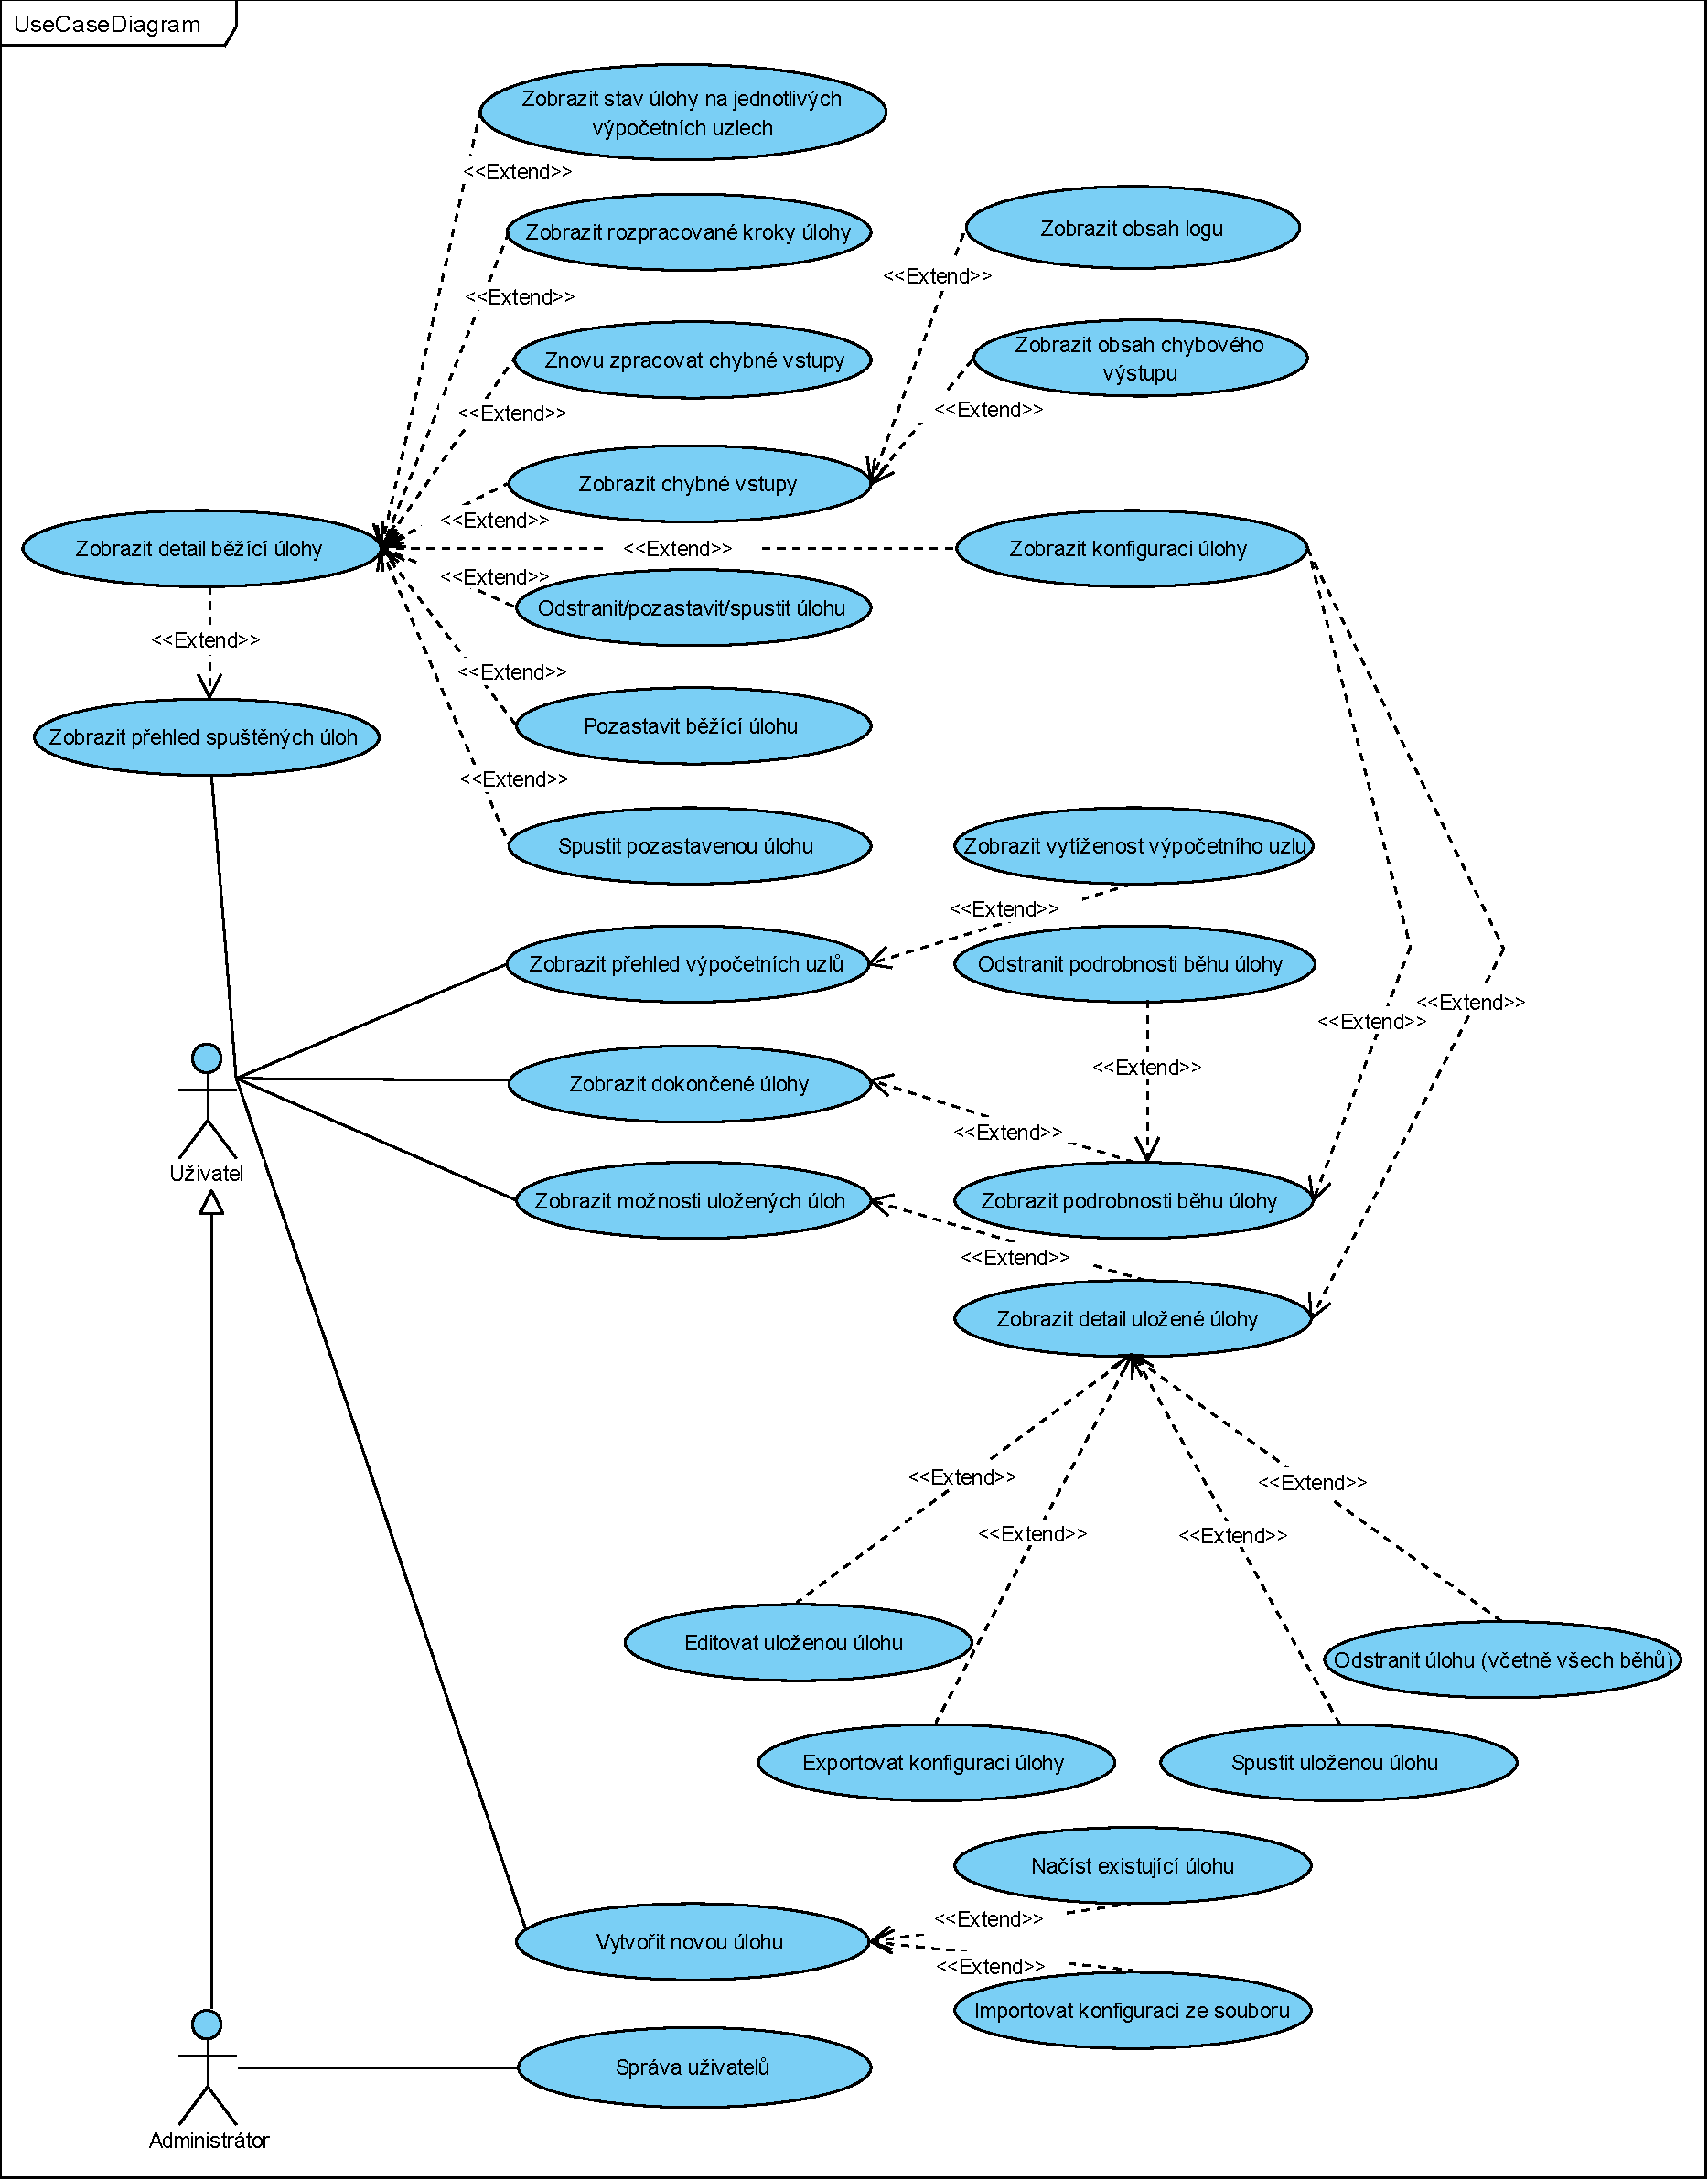
\includegraphics{images/UseCaseDiagram.pdf}
    }
    \caption{\label{obr:useCaseDiagram} {\it Diagram případů užití.}}
\end{center}
\end{figure}

\begin{table}[H]
\centering
    \scalebox{0.83}{
    	\begin{tabular}{Sl|Sl|Sl|Sl|Sl|Sl}
            \midrule
    		\bf	Identifikátor & \multicolumn{5}{l}{VNU} \\ \hline
    		\bf Název & \multicolumn{5}{l}{Vytvoření nové úlohy} \\ \hline
    		\bf Popis & \multicolumn{5}{l}{Uživatel U vytvoří novou úlohu ke zpracování} \\ \hline
    		\bf Priorita & 2 = střední & \multicolumn{2}{l|}{\bf Frekvence} & \multicolumn{2}{l}{Několikrát za týden} \\ \hline
    		 \textbf{\makecell{Počáteční\\ podmínky}} & \multicolumn{5}{l}{Uživatel U je přihlášen do systému.} \\ \hline
    		\textbf{\makecell{Koncové \\ podmínky}} & \multicolumn{5}{l}{Nová úloha byla vytvořena.} \\ \hline
    		\bf Aktéři & \multicolumn{5}{l}{Uživatel U} \\ \hline
    		\multirow{6}{*}{\textbf{\makecell{Základní \\ posloupnost}}} & \bf Krok & \multicolumn{4}{l}{\bf Činnost} \\ \cline{2-6}
    		& 1 & \multicolumn{4}{l}{U vyplní údaje o nové úloze.} \\ \cline{2-6}
    		& 2 & \multicolumn{4}{l}{\makecell[l]{\textcolor{red}{\bf Když} je některá informace špatně zadaná: \\ 2.1. Systém zobrazí chybové hlášení a přejde na krok 1.}} \\ \cline{2-6}
    		& 3 & \multicolumn{4}{l}{\makecell[l]{Systém přidá novou úlohu a zobrazí hlášení \\ o úspěšném provedení operace.}} \\ \hline
    		\multirow{2}{*}{\textbf{\makecell{Alternativní \\ posloupnost}}}  & \bf Krok & \multicolumn{4}{l}{\bf Činnost} \\ \cline{2-6}
    		& 1 & \multicolumn{4}{l}{U může kdykoliv opustit formulář pro vytvoření nové úlohy.} \\ \hline
    		\multirow{6}{*}{\textbf{\makecell{Výjimky \\ z normální \\ posloupnosti}}} & \bf Číslo & \multicolumn{3}{l|}{\bf Popis} & \textbf{\makecell{Ošetřeno \\ krokem}} \\ \cline{2-6}
    		& 1 & \multicolumn{3}{l|}{\makecell[l]{U nevyplnil všechny povinné údaje ve formuláři \\ a zvolil vytvoření nové úlohy.}} & 2 \\ \cline{2-6}
    		& 2 & \multicolumn{3}{l|}{\makecell[l]{U vyplnil některou položku chybně a zvolil \\ vytvoření nové úlohy.}} & 2 \\ \hline
    		\bf Poznámky & \multicolumn{5}{l}{~} \\ \hline
    	\end{tabular}
	}
	\caption{\label{table:useCaseDetail__createNewTask} {\it Detail případu užití -- Vytvořit novou úlohu.}}
\end{table}

\begin{table}[H]
\centering
    \scalebox{0.83}{
    	\begin{tabular}{Sl|Sl|Sl|Sl|Sl|Sl}
            \midrule
    		\bf	Identifikátor & \multicolumn{5}{l}{ZZCHV} \\ \hline
    		\bf Název & \multicolumn{5}{l}{Znovu zpracovat chybné vstupy} \\ \hline
    		\bf Popis & \multicolumn{5}{l}{Uživatel U spustí opětovné zpracování chybných vstupů.} \\ \hline
    		\bf Priorita & 2 = střední & \multicolumn{2}{l|}{\bf Frekvence} & \multicolumn{2}{l}{Několikrát za týden} \\ \hline
    		 \textbf{\makecell{Počáteční\\ podmínky}} & \multicolumn{5}{l}{\makecell[l]{Uživatel U je přihlášen do systému a v systému existuje \\ nedokončená úloha s chybným vstupem na některém výpočetním uzlu.}} \\ \hline
    		\textbf{\makecell{Koncové \\ podmínky}} & \multicolumn{5}{l}{Zpracování chybných vstupů bylo spuštěno.} \\ \hline
    		\bf Aktéři & \multicolumn{5}{l}{Uživatel U} \\ \hline
    		\multirow{11}{*}{\textbf{\makecell{Základní \\ posloupnost}}} & \bf Krok & \multicolumn{4}{l}{\bf Činnost} \\ \cline{2-6}
    		& 1 & \multicolumn{4}{l}{U si zobrazí přehled spuštěných úloh.} \\ \cline{2-6}
    		& 2 & \multicolumn{4}{l}{U si zobrazí detail konkrétní úlohy.} \\ \cline{2-6}
    		& 3 & \multicolumn{4}{l}{\makecell[l]{U vybere ze seznamu konkrétní výpočetní uzel, na kterém \\ chce opětovné zpracování chybných vstupů spustit.}} \\ \cline{2-6}
    		& 4 & \multicolumn{4}{l}{\makecell[l]{\textcolor{red}{\bf Když} úloha na daném výpočetním uzlu běží: \\ 4.1. Systém zařadí chybné vstupy do fronty nezpracovaných \\ vstupů na daném uzlu. \\ \textcolor{red}{\bf Když} úloha na daném výpočetním uzlu neběží: \\  4.2. Systém zařadí daný krok úlohy do fronty proveditelných \\ kroků. Při jeho následném spuštění zajistí zařazení chybných \\ vstupů do fronty nezpracovaných vstupů na daném uzlu.}} \\ \cline{2-6}
    		& 5 & \multicolumn{4}{l}{\makecell[l]{Systém zobrazí hlášení o úspěšném provedení operace.}} \\ \hline
    		\multirow{2}{*}{\textbf{\makecell{Alternativní \\ posloupnost}}}  & \bf Krok & \multicolumn{4}{l}{\bf Činnost} \\ \cline{2-6}
    		& 1,2,3 & \multicolumn{4}{l}{\makecell[l]{U se může kdykoliv vrátit k předchozímu kroku \\ nebo pokračovat jiným případem užití.}} \\ \hline
    		\bf Poznámky & \multicolumn{5}{l}{~} \\ \hline
    	\end{tabular}
	}
	\caption{\label{table:useCaseDetail__repeatErrInputs} {\it Detail případu užití -- Znovu zpracovat chybné vstupy.}}
\end{table}

\begin{table}[H]
\centering
    \scalebox{0.83}{
    	\begin{tabular}{Sl|Sl|Sl|Sl|Sl|Sl}
            \midrule
    		\bf	Identifikátor & \multicolumn{5}{l}{OBU} \\ \hline
    		\bf Název & \multicolumn{5}{l}{Odstranit rozpracovanou úlohu} \\ \hline
    		\bf Popis & \multicolumn{5}{l}{Uživatel U odstraní rozpracovaný běh úlohy.} \\ \hline
    		\bf Priorita & 2 = střední & \multicolumn{2}{l|}{\bf Frekvence} & \multicolumn{2}{l}{Několikrát za měsíc} \\ \hline
    		 \textbf{\makecell{Počáteční\\ podmínky}} & \multicolumn{5}{l}{\makecell[l]{Uživatel U je přihlášen do systému \\ a v systému existuje nedokončená úloha.}} \\ \hline
    		\textbf{\makecell{Koncové \\ podmínky}} & \multicolumn{5}{l}{Rozpracovaná úloha byla odstraněna.} \\ \hline
    		\bf Aktéři & \multicolumn{5}{l}{Uživatel U} \\ \hline
    		\multirow{6}{*}{\textbf{\makecell{Základní \\ posloupnost}}} & \bf Krok & \multicolumn{4}{l}{\bf Činnost} \\ \cline{2-6}
    	    & 1 & \multicolumn{4}{l}{U si zobrazí přehled spuštěných úloh.} \\ \cline{2-6}
    		& 2 & \multicolumn{4}{l}{U si zobrazí detail konkrétní úlohy.} \\ \cline{2-6}
    		& 3 & \multicolumn{4}{l}{\makecell[l]{\textcolor{red}{\bf Když} úloha na žádném výpočetním uzlu neběží: \\ 3.1. U pokračuje krokem 6.}} \\ \cline{2-6}
    		& 4 & \multicolumn{4}{l}{\makecell[l]{U pozastaví úlohu na všech výpočetních uzlech.}} \\ \hline
			& 5 & \multicolumn{4}{l}{\makecell[l]{Systém provede pozastavení úlohy na všech výpočetních \\ uzlech a zobrazí hlášení o úspěšném pozastavení úlohy.}} \\ \hline
    		& 6 & \multicolumn{4}{l}{\makecell[l]{U provede odstranění běhu úlohy.}} \\ \hline
    		& 7 & \multicolumn{4}{l}{\makecell[l]{Systém odstraní rozpracovaný běh úlohy a zobrazí hlášení \\ o úspěšném provedení operace.}} \\ \hline
    		\multirow{2}{*}{\textbf{\makecell{Alternativní \\ posloupnost}}}  & \bf Krok & \multicolumn{4}{l}{\bf Činnost} \\ \cline{2-6}
    		& 1,2 & \multicolumn{4}{l}{\makecell[l]{U se může kdykoliv vrátit k předchozímu kroku \\ nebo pokračovat jiným případem užití.}} \\ \hline
    		& 6 & \multicolumn{4}{l}{\makecell[l]{U může pokračovat jiným případem užití.}} \\ \hline
    		\bf Poznámky & \multicolumn{5}{l}{~} \\ \hline
    	\end{tabular}
	}
	\caption{\label{table:useCaseDetail__deleteUncompleteTask} {\it Detail případu užití -- Odstranit rozpracovanou úlohu.}}
\end{table}

Další případy užití jsou vzhledem ke složitosti uživatelského rozhraní pro jejich provedení popsány přímo v následující podkapitole, která se zabývá jeho návrhem.

%-----------------------------------------------------------------------------------------------------------------

\section{Návrh grafického uživatelského rozhraní}
\label{section:wireframeDesign}

Pro návrh grafického uživatelského rozhraní byl využit online nástroj Balsamiq, který je detailně popsán v kapitole \ref{subsection:technology_Balsamiq}. Návrh byl prováděn ve 4 iteracích. Na první schůzce, týkající se návrhu uživatelského rozhraní, byl vytvořen hrubý náčrt základních částí aplikace. Tento papírový náčrt byl následně využit pro návrh  wireframe pomocí nástroje Balsamiq, přičemž do něj byly zapracovány všechny dosavadní požadavky. V každé další iteraci byly vytvořené návrhy upravovány dle upřesňujících požadavků.

Při návrhu jednotlivých wireframe byly rovněž blíže specifikovány požadavky na data, která mají být zobrazována, a byly tak dále upřesněny jednotlivé případy užití. Nejdůležitější a na návrh nejnáročnější části grafického uživatelského rozhraní po poslední iteraci jsou popsány v této kapitole. Zbývající wireframe jsou pak pro úplnost obsaženy v příloze~\ref{appendix:otherWireframes}.

\subsection*{Detail běžící úlohy}
\label{subsection:runTaskDetail}

Výsledný návrh zobrazení detailu běžící úlohy je možné vidět na obrázku \ref{obr:wireframe_taskDetail}. Ve spodní třetině obrazovky bude uvedena tabulka se všemi uzly, na kterých byla úloha spuštěna. U každého uzlu bude uveden jeho název, běžící krok, doba běhu a doba čekání. Doba čekání bude zahrnovat celkovou dobu, kdy na daném výpočetním uzlu úloha neběžela, ať už z~důvodu čekání na uvolnění výpočetního uzlu, nebo z důvodu čekání na opětovné spuštění zpracování chybných vstupů. Dále bude u každého uzlu uvedeno, kolik vstupů bylo z jejich celkového počtu již zpracováno, a stav úlohy, který může být následující:
\begin{itemize}
    \item Běží -- úloha je na daném uzlu spuštěna, žádné chyby nenastaly,
    \item Běží/chyba -- úloha na daném uzlu běží, avšak zpracování jednoho či více souborů skončilo s chybou,
    \item Chyba --  úloha na daném uzlu již neběží, poslední prováděný krok nebyl úspěšně dokončen, protože zpracování jednoho či více vstupů skončilo s chybou,
    \item Čeká -- krok úlohy čeká na uvolnění výpočetního uzlu, který je obsazen jinou úlohou,
    \item Pozastaveno -- zpracování úlohy na daném uzlu bylo pozastaveno uživatelem,
    \item Dokončeno -- úloha byla na daném uzlu úspěšně dokončena.
\end{itemize}
U každého uzlu bude možné v závislosti na stavu, v jakém se zpracování úlohy na daném uzlu nachází, provádět různé operace. V případě chyby bude aplikace poskytovat přehled všech vstupních souborů, jejichž zpracování skončilo s chybou. U každého chybného vstupu bude uveden obsah logu nebo chybového výstupu v závislosti na nastavení při vytváření úlohy. Úlohu bude dále možné na daném uzlu pozastavit, spustit, případně opětovně spustit zpracování chybných vstupů. V případě, že bude úloha pozastavena, budou při následném spuštění zpracovány pouze nezpracované vstupy. Vynechány tedy budou již zpracované a~chybné vstupy. Tento případ užití je detailně popsán v tabulce \ref{table:useCaseDetail__repeatErrInputs}.

Uprostřed se bude nacházet tabulka, ve které bude zobrazen přehled všech kroků úlohy. U každého kroku bude uveden celkový počet zpracovaných vstupů na všech výpočetních uzlech v poměru k celkovému počtu vstupů. Tabulka bude dále obsahovat nejdůležitější stav daného kroku, který bude získán ze stavu daného kroku na jednotlivých výpočetních uzlech seřazených dle následujících priorit v pořadí od nejvyšší po nejnižší:
\begin{enumerate}
    \item Chyba
    \item Běží/Chyba
    \item Pozastaveno
    \item Čeká
    \item Běží
    \item Dokončeno
\end{enumerate}
Uživatel bude mít dále v této části možnost zobrazit si konfiguraci úlohy, pozastavit úlohu na všech výpočetních uzlech, případně její zpracování na všech výpočetních uzlech opětovně spustit nebo celý běh úlohy odstranit.

V horní části obrazovky bude uveden čas spuštění úlohy, uplynulý čas od jejího spuštění, počet úspěšně dokončených kroků na všech výpočetních uzlech, název posledního úspěšně dokončeného kroku a počet uzlů, na kterých úloha v současné době běží. Dále zde bude informace o celkovém stavu úlohy získaná ze stavu rozpracovaných kroků dle priorit uvedených v předchozím odstavci.

\begin{figure}[H]
\begin{center}
    \scalebox{0.78}
    {   
        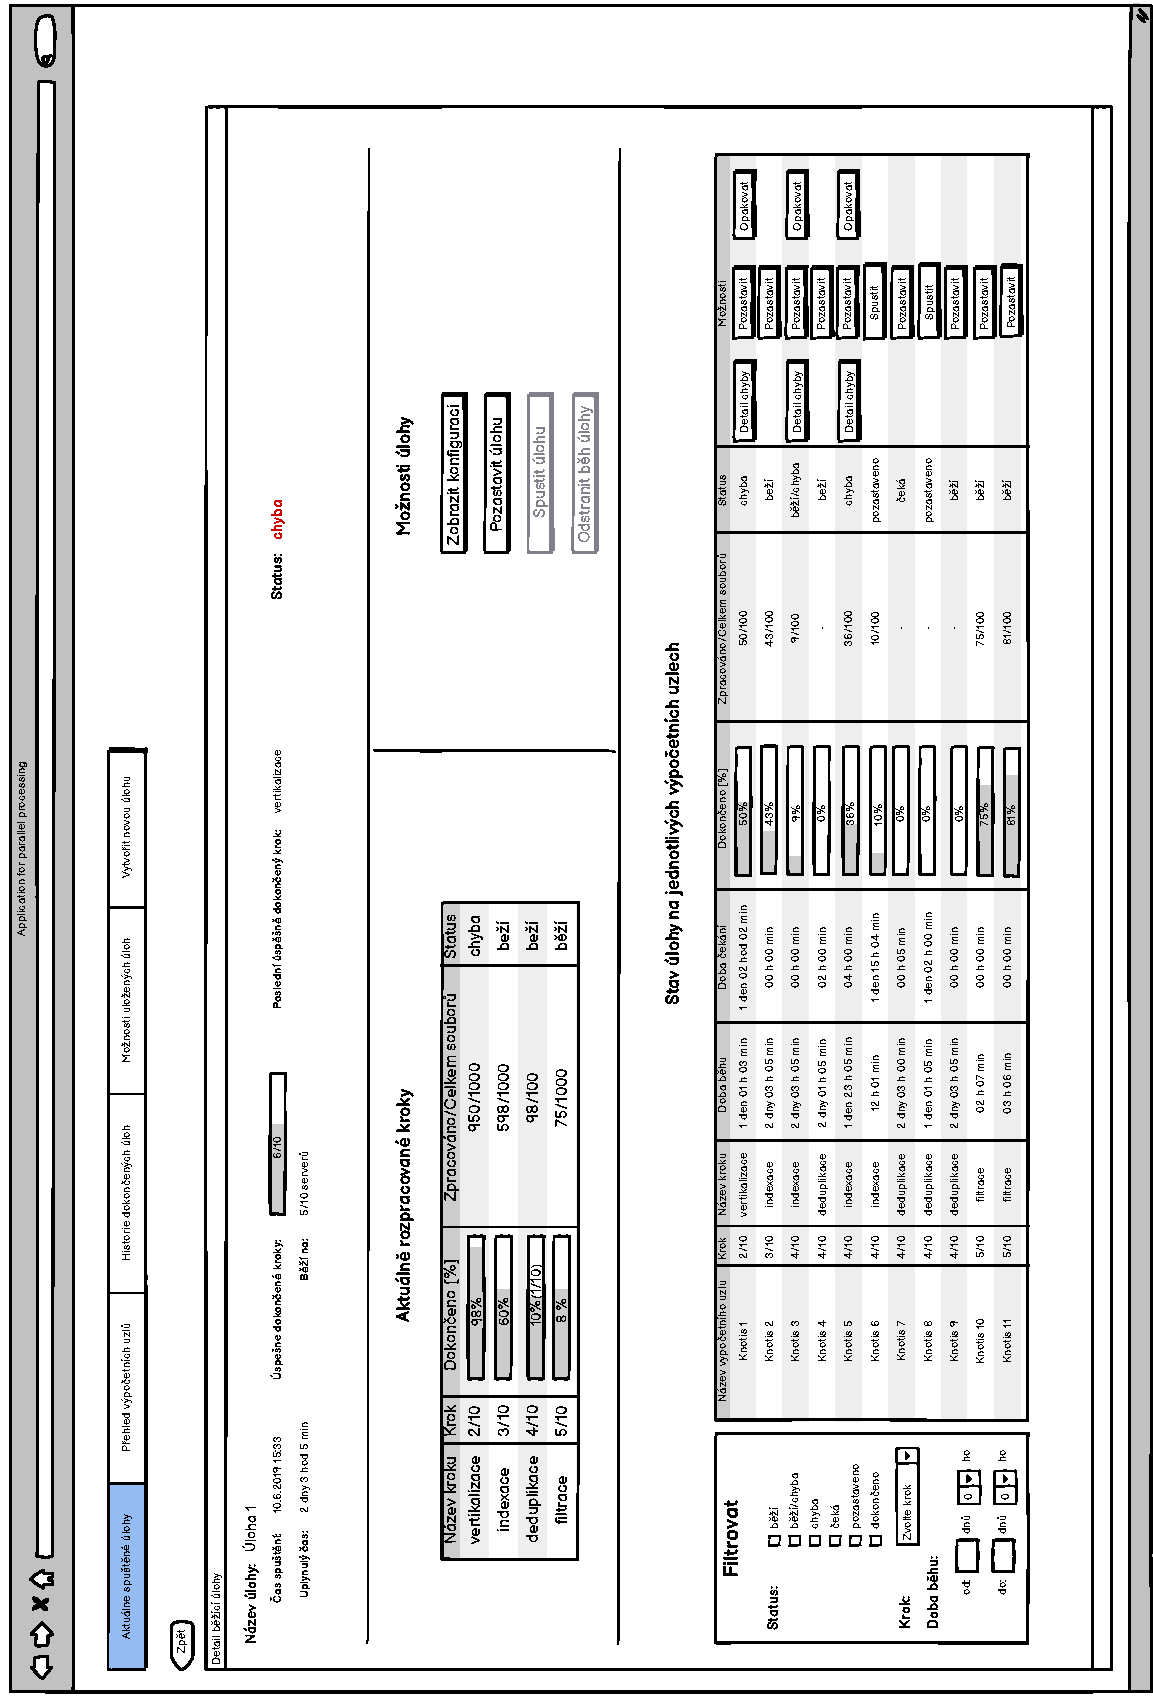
\includegraphics{images/wireframe_taskDetail.pdf}
    }
    \caption{\label{obr:wireframe_taskDetail} {\it Návrh obrazovky -- Detail běžící úlohy.}}
\end{center}
\end{figure}

\subsection*{Detail dokončené úlohy}

Návrh obrazovky pro detail dokončené úlohy je možné vidět na obrázcích \ref{obr:wireframe_finishedTaskDetail_1} a \ref{obr:wireframe_finishedTaskDetail_2}. V~horní části bude uvedeno datum spuštění, datum dokončení, počet uzlů, na kterých byla úloha spuštěna, a doba běhu úlohy, tj. čas od jejího spuštění po úspěšné dokončení úlohy na všech výpočetních uzlech. Dále zde bude uveden celkový čas výpočtu, který bude odpovídat součtu délek výpočtů na všech výpočetních uzlech. Obdobným způsobem bude dopočítána i celková doba čekání. Uživatel bude mít také možnost zobrazit si konfiguraci, s jakou byla úloha spuštěna, případně záznam o jejím běhu odstranit.

Uprostřed se bude nacházet graf celkové doby trvání úlohy na jednotlivých výpočetních uzlech. Níže bude možné zobrazit pro každý krok úlohy statistiky o jeho běhu ve formě grafů. Na prvním grafu bude zobrazena doba provádění daného kroku na každém uzlu. Další graf bude znázorňovat minimální, průměrnou a maximální dobu zpracování jednoho vstupu. Ve statistikách budou dále zahrnuty grafy minimálního, průměrného a maximálního vytížení procesoru a využití paměti RAM. 

\subsection*{Vytvoření nové úlohy}
\label{subsection:newTaskForm}

Další náročnější částí návrhu byl formulář pro vytvoření nové úlohy, jehož finální podobu je možné vidět na obrázku \ref{obr:wireframe_newTaskForm}. Kromě zadání zcela nové úlohy bude mít uživatel možnost nahrát konfiguraci ze souboru, případně načíst existující konfiguraci dříve spuštěné nebo uložené úlohy. 

Uživatel bude zadávat název úlohy, specifikovat výpočetní uzly, na kterých má být úloha spuštěna, a definovat jednotlivé kroky úlohy. U každého kroku bude nutné zadat jeho název, cestu k spouštěnému programu, typ vstupu a výstupu, kterým může být soubor, složka, složka souborů nebo složka složek. Dále bude nutné specifikovat název argumentu příkazové řádky spouštěného programu pro zadání vstupu/výstupu  a cestu ke vstupu/výstupu. Následně bude nutné zadat počet procesů, ve kterých má být zpracování na každém uzlu spuštěno, a regulární výraz, který se aplikuje na cestu ke vstupu. Jednotlivé skupiny znaků, které vzniknou aplikací tohoto regulárního výrazu, mohou být využity ve specifikaci cesty k~výstupu, logu případně ostatních parametrů pomocí znaku \textit{\$x}, kde \textit{x} je číslo skupiny znaků vybrané regulárním výrazem, kterou má být znak \textit{\$x} nahrazen.

U každého kroku bude dále nezbytné specifikovat maximální dobu zpracování jednoho vstupu. Při překročení této doby bude zpracování daného vstupu ukončeno s chybou. Pokračovat se bude v pořadí dalším nezpracovaným vstupem. Následně budou definovány validace, které mají být provedeny po každém zpracovaném vstupu. Tyto validace budou detailně popsány v následující kapitole \ref{section:validationDesign}. U každého kroku bude dále možné specifikovat, zda má být v případě chyby uložen obsah chybového logu nebo obsah standardního chybového výstupu spuštěného programu a zda má být tento krok synchronizován.

\begin{figure}[H]
\begin{center}
    \scalebox{1.0}
    {   
        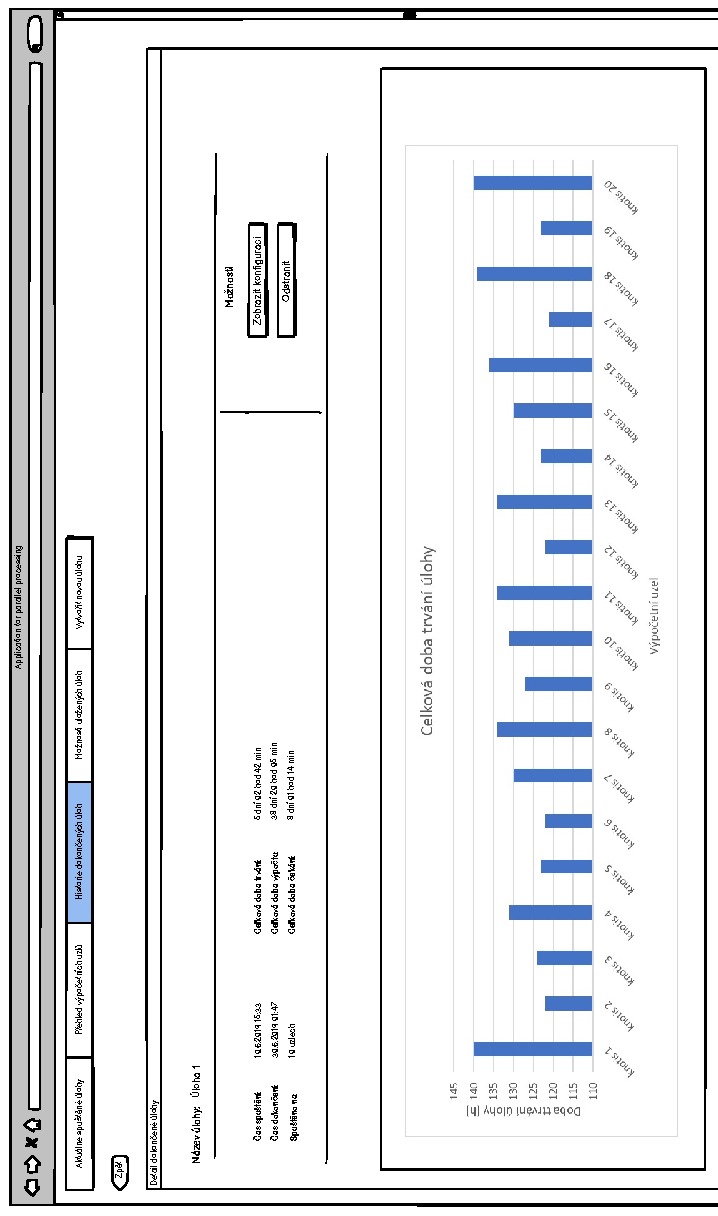
\includegraphics{images/wireframe_finishedTaskDetail_1.pdf}
    }
    \caption{\label{obr:wireframe_finishedTaskDetail_1} {\it Návrh obrazovky (horní část) -- Detail dokončené úlohy.}}
\end{center}
\end{figure}

\begin{figure}[H]
\begin{center}
    \scalebox{1.0}
    {   
        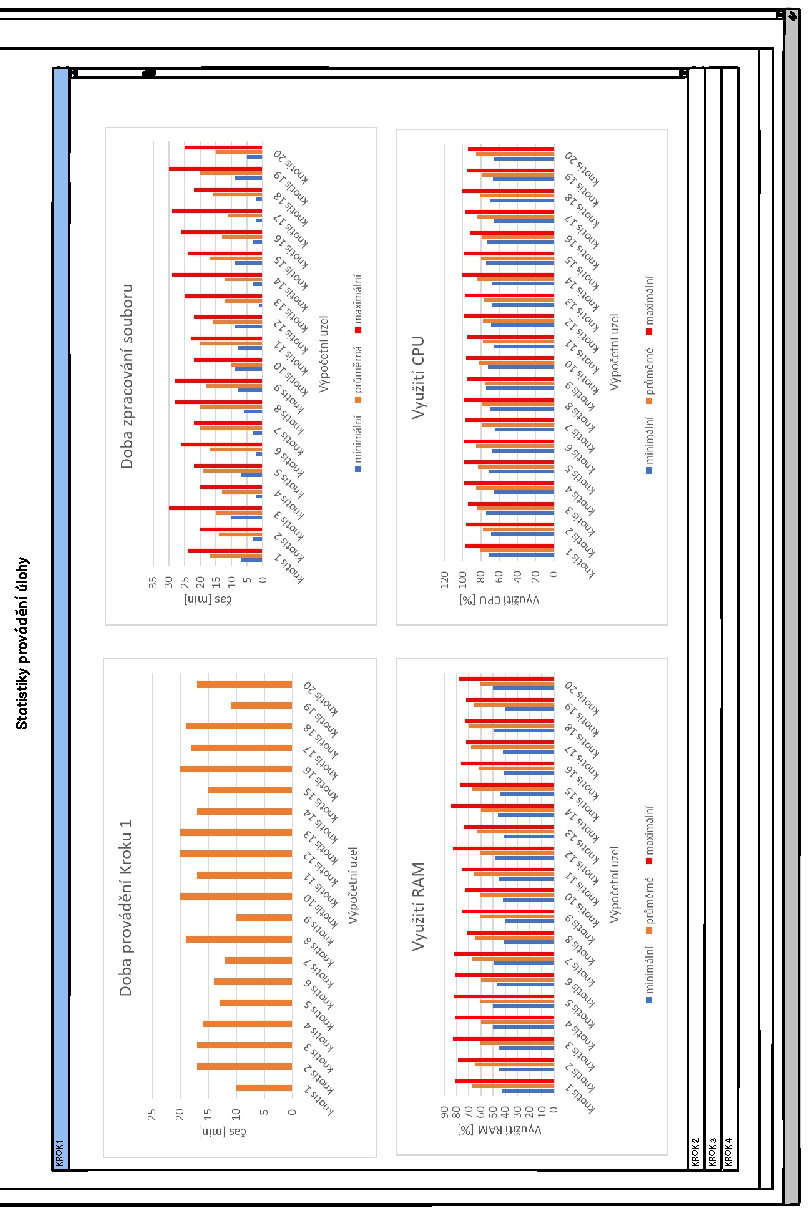
\includegraphics{images/wireframe_finishedTaskDetail_2.pdf}
    }
    \caption{\label{obr:wireframe_finishedTaskDetail_2} {\it Návrh obrazovky (dolní část) -- Detail dokončené úlohy.}}
\end{center}
\end{figure}

\begin{figure}[H]
\begin{center}
    \scalebox{0.8}
    {   
        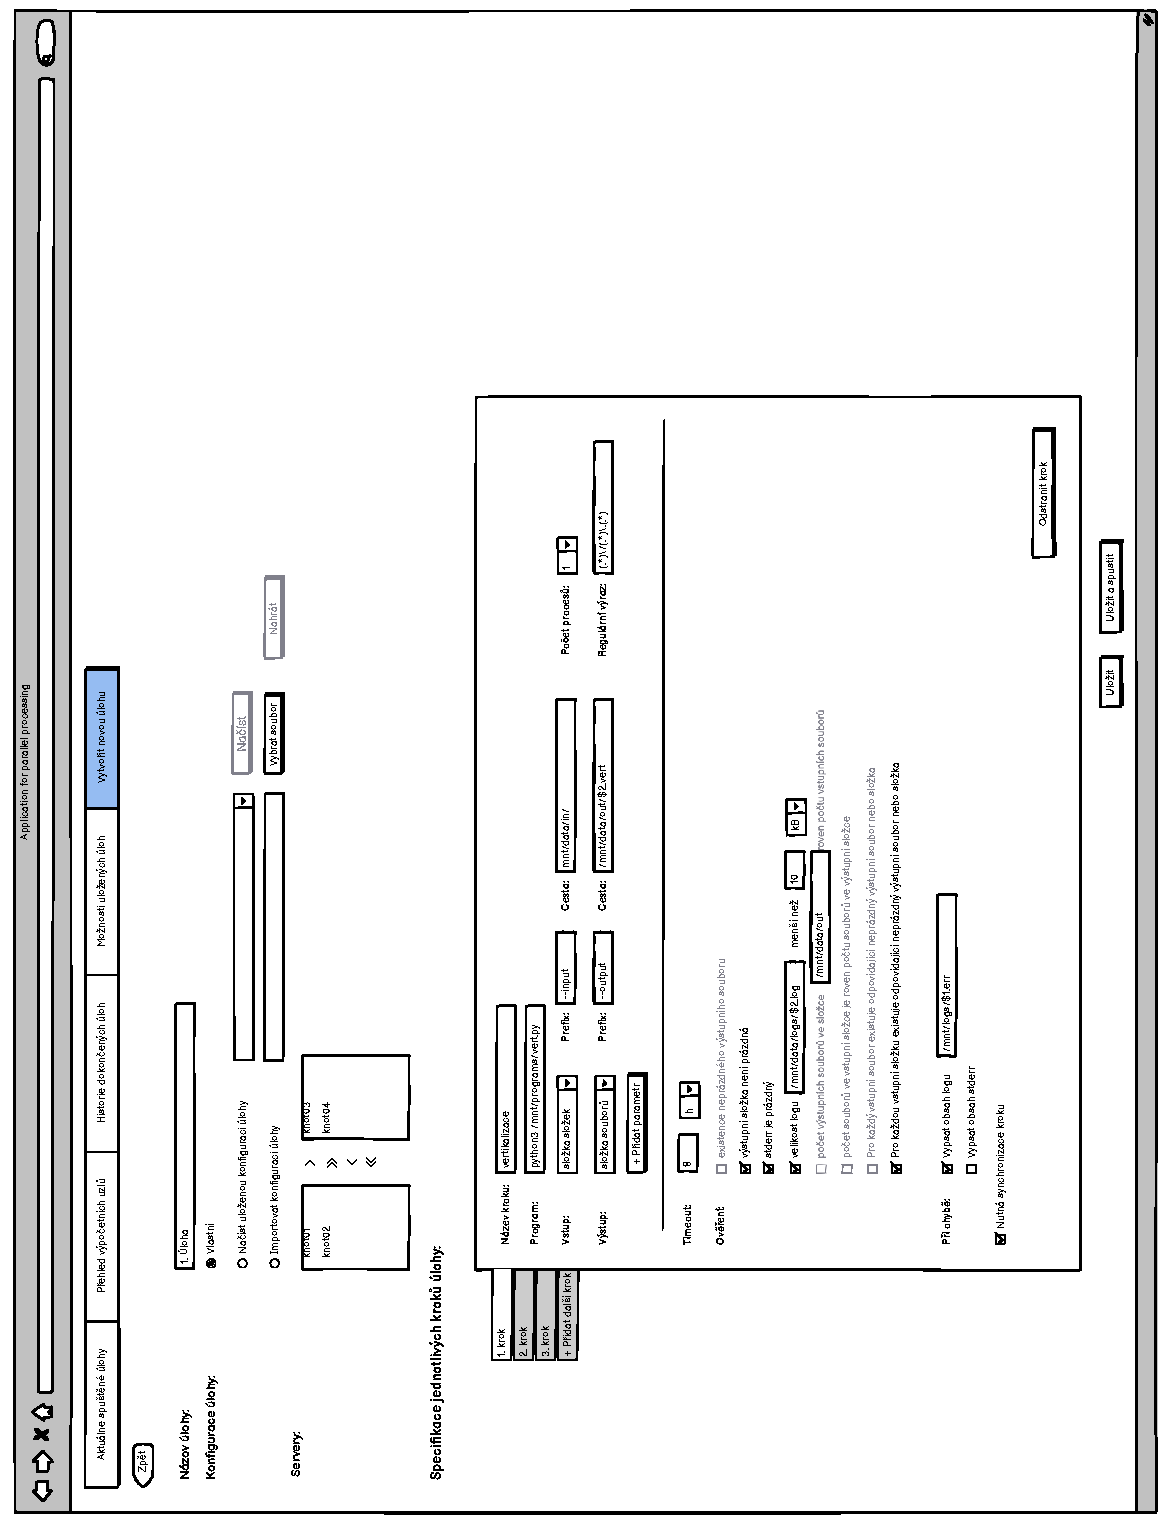
\includegraphics{images/wireframe_newTaskForm.pdf}
    }
    \caption{\label{obr:wireframe_newTaskForm} {\it Návrh obrazovky -- Vytvoření nové úlohy.}}
\end{center}
\end{figure}


%-----------------------------------------------------------------------------------------------------------------

\section{Validace výstupů úlohy}
\label{section:validationDesign}

Jak bylo uvedeno v kapitole \ref{subsection:newTaskForm}, u každého kroku úlohy bude možné specifikovat validace, které mají být provedeny po každém zpracovaném vstupu s cílem ověřit, zda bylo zpracování daného vstupu úspěšné.

Na základě získaných požadavků bude nutné rozlišit 4 typy vstupů a výstupů. Typ vstupu určuje způsob reprezentace zadané vstupní cesty následovně:

\begin{itemize}
    \item Soubor -- vstupní cesta reprezentuje vstupní soubor, se kterým má být program spuštěn,
    \item Složka -- vstupní cesta reprezentuje vstupní složku, se kterou má být program spuštěn,
    \item Složka souborů -- vstupní cesta reprezentuje složku obsahující soubory, přičemž program má být spuštěn samostatně s každým souborem ve složce,
    \item Složka složek -- vstupní cesta reprezentuje složku obsahující podsložky, přičemž program má být spuštěn samostatně s každou podsložkou ve složce.
\end{itemize}

Analogicky typ výstupu určuje způsob reprezentace zadané výstupní cesty:

\begin{itemize}
    \item Soubor -- výstupní cesta reprezentuje cestu k výstupnímu souboru, se kterým má být program spuštěn,
    \item Složka -- výstupní cesta reprezentuje cestu k výstupní složce, se kterou má být program spuštěn, přičemž program může být opakovaně spouštěn s různými vstupy, ale stejnou výstupní složkou,
    \item Složka souborů -- výstupní cesta reprezentuje cestu ke složce s výstupními soubory, tato cesta je typicky zadána s parametrem -- pro každý vstup je tak získána cesta k~odpovídajícímu výstupnímu souboru, což je detailně popsáno v podkapitole \ref{subsection:newTaskForm},
    \item Složka složek -- výstupní cesta reprezentuje cestu ke složce s výstupními podsložkami, tato cesta je typicky zadána s parametrem -- pro každý vstup je tak získána cesta k~odpovídající výstupní složce stejně jako v předchozím případě.
\end{itemize}

Z výše uvedeného je zřejmé, že některé kombinace vstupů a výstupů nejsou přípustné. Pokud je program spuštěn jen jednou -- vstupem je tedy soubor nebo složka, nemůže být výstupem složka souborů nebo složka složek. Stejně tak pokud je vstupem složka souborů nebo složka složek, nemůže být výstupem soubor, protože by se jeho obsah s každým spuštěným vstupem neustále přepisoval. 

Validace, které je možné u daného kroku provést, závisí vždy na kombinaci typu vstupu a typu výstupu daného kroku. Možné validace pro přípustné kombinace jsou uvedeny v~tabulce \ref{table:input_output_combination}.

\setlength\cellspacetoplimit{4pt}
\setlength\cellspacebottomlimit{4pt}

\begin{table}[H]
\centerline {
    \begin{adjustbox}{angle=90}\scalebox{0.66} {
	\begin{tabular}{Sc|Sl|Sl|Sl|Sl}
    	\bottomrule
          \multirow{2}{*}{Typ vstupu} & \multicolumn{4}{c}{Typ výstupu} \\ \cline{2-5}
            & \multicolumn{1}{c|}{Soubor} &  \multicolumn{1}{c|}{Složka} & \multicolumn{1}{c|}{Složka souborů} & \multicolumn{1}{c}{Složka složek} \\
        \midrule
			\multirow{6}{*}{Soubor}	& 
			    \tabitem existence výstupního souboru & \tabitem neprázdná výstupní složka & \multicolumn{1}{c|}{\multirow{6}{*}{X}} &  \multicolumn{1}{c}{\multirow{6}{*}{X}}	\\
			&   \tabitem standardní chybový výstup & \tabitem standardní chybový výstup &  & \\
			&    \hspace{1em} je prázdný & \hspace{1em} je prázdný &  & \\ 
			&   \tabitem velikost logu menší než & \tabitem velikost logu menší než & & \\
			&   \hspace{1em} zvolená hodnota & \hspace{1em} zvolená hodnota & & \\ \hline
			\multirow{10}{*}{Složka}	& 
			    \tabitem existence výstupního souboru & \tabitem neprázdná výstupní složka & \multicolumn{1}{c|}{\multirow{10}{*}{X}} &  \multicolumn{1}{c}{\multirow{10}{*}{X}}	\\
			&   \tabitem standardní chybový výstup & \tabitem standardní chybový výstup &  & \\
			&    \hspace{1em} je prázdný & \hspace{1em} je prázdný &  & \\ 
			&   \tabitem velikost logu menší než & \tabitem velikost logu menší než & & \\
			&   \hspace{1em} zvolená hodnota & \hspace{1em} zvolená hodnota & & \\
			&  & \tabitem počet souborů ve vstupní  & & \\
			&  & \hspace{1em} složce je roven počtu souborů & & \\ 
			&  & \hspace{1em} ve výstupní složce  & & \\ \hline
			\multirow{14}{*}{Složka souborů}	& 
			     \multicolumn{1}{c|}{\multirow{14}{*}{X}} & \tabitem neprázdná výstupní složka & \tabitem neprázdná výstupní složka & \tabitem neprázdná výstupní složka \\
			& & \tabitem standardní chybový výstup & \tabitem standardní chybový výstup & \tabitem standardní chybový výstup \\ 
			& &  \hspace{1em} je prázdný &  \hspace{1em} je prázdný & \hspace{1em} je prázdný \\ 
			& & \tabitem velikost logu menší než & \tabitem velikost logu menší než  & \tabitem velikost logu menší než \\
			& & \hspace{1em} zvolená hodnota & \hspace{1em} zvolená hodnota  & \hspace{1em} zvolená hodnota \\
			& & & \tabitem pro každý vstupní soubor & \tabitem pro každý vstupní soubor \\
			& & & \hspace{1em} existuje odpovídající & \hspace{1em} existuje odpovídající \\
			& & & \hspace{1em} neprázdný výstupní soubor & \hspace{1em} neprázdná výstupní složka \\
			& & & \tabitem Počet souborů ve výstupní & \tabitem Počet složek ve výstupní  \\
			& & & \hspace{1em} složce je roven počtu souborů & \hspace{1em}složce je roven počtu souborů \\
			& & & \hspace{1em} ve vstupní složce & \hspace{1em} ve výstupní složce \\\hline
			\multirow{14}{*}{Složka souborů}	& 
			     \multicolumn{1}{c|}{\multirow{14}{*}{X}} & \tabitem neprázdná výstupní složka & \tabitem neprázdná výstupní složka & \tabitem neprázdná výstupní složka \\
			& & \tabitem standardní chybový výstup & \tabitem standardní chybový výstup & \tabitem standardní chybový výstup \\ 
			& &  \hspace{1em} je prázdný &  \hspace{1em} je prázdný & \hspace{1em} je prázdný \\ 
			& & \tabitem velikost logu menší než & \tabitem velikost logu menší než  & \tabitem velikost logu menší než \\
			& & \hspace{1em} zvolená hodnota & \hspace{1em} zvolená hodnota  & \hspace{1em} zvolená hodnota \\
			& & & \tabitem ke každé vstupní složce & \tabitem ke každé vstupní složce \\
			& & & \hspace{1em} existuje odpovídající & \hspace{1em} existuje odpovídající \\
			& & & \hspace{1em} neprázdný výstupní soubor & \hspace{1em} neprázdná výstupní složka \\
			& & & \tabitem Počet souborů ve výstupní & \tabitem Počet složek ve výstupní  \\
			& & & \hspace{1em} složce je roven počtu složek & \hspace{1em}složce je roven počtu složek \\
			& & & \hspace{1em} ve vstupní složce & \hspace{1em} ve vstupní složce \\\hline
	\end{tabular}}
	\end{adjustbox}
      }
      \caption{\label{table:input_output_combination} {\it Přehled validací, které je možné u daného kroku provést v závislosti na typu vstupu a výstupu.}}
\end{table}

%-----------------------------------------------------------------------------------------------------------------

\section{Entity Relationship diagram}
\label{section:databaseDesign}

Na základě požadavků na aplikaci byl proveden návrh uložení dat v databázi na centrálním uzlu. Pro jeho modelování byl využit Entity Relationship diagram, který je možné vidět na obrázku \ref{obr:ER_diagram}.

Z diagramu je zřejmé, že v databázi budou ukládány informace o výpočetních uzlech, na kterých bude probíhat zpracování úlohy, a záznamy o jejich vytíženosti. Entitní množina pro ukládání těchto záznamů obsahuje kromě hodnoty vytíženosti v procentech a data, ke kterému se daný záznam vztahuje, i typ záznamu, který označuje, jakému časovému úseku záznam odpovídá. Může se jednat o 5vteřinový, minutový, půlhodinový, hodinový, 12hodinový nebo denní záznam. Tyto typy záznamů byly zvoleny tak, aby v každém rozsahu, v jakém bude využití výpočetního uzlu zobrazováno, bylo v grafu obsaženo dostatečné množství dat. Jednotlivé rozsahy, v jakých bude vytíženost uzlu zobrazována, jsou popsány v kapitole \ref{section:analysisANdUseCaseDiagram}. 

V databázi budou dále ukládány informace o vytvářených úlohách a data, která jsou nezbytná pro zobrazení statistik o využití systémových prostředků pro každý běh úlohy. Entitní množina pro ukládání těchto dat bude obsahovat záznamy o běhu každého kroku úlohy na každém výpočetním uzlu. Ke všem těmto entitám budou ukládány chyby, které při zpracování nastaly. Při spuštění opětovného zpracování chybných vstupů budou tyto záznamy o~chybách vymazány.

\begin{figure}[H]
\begin{center}
    \scalebox{0.5}
    {
        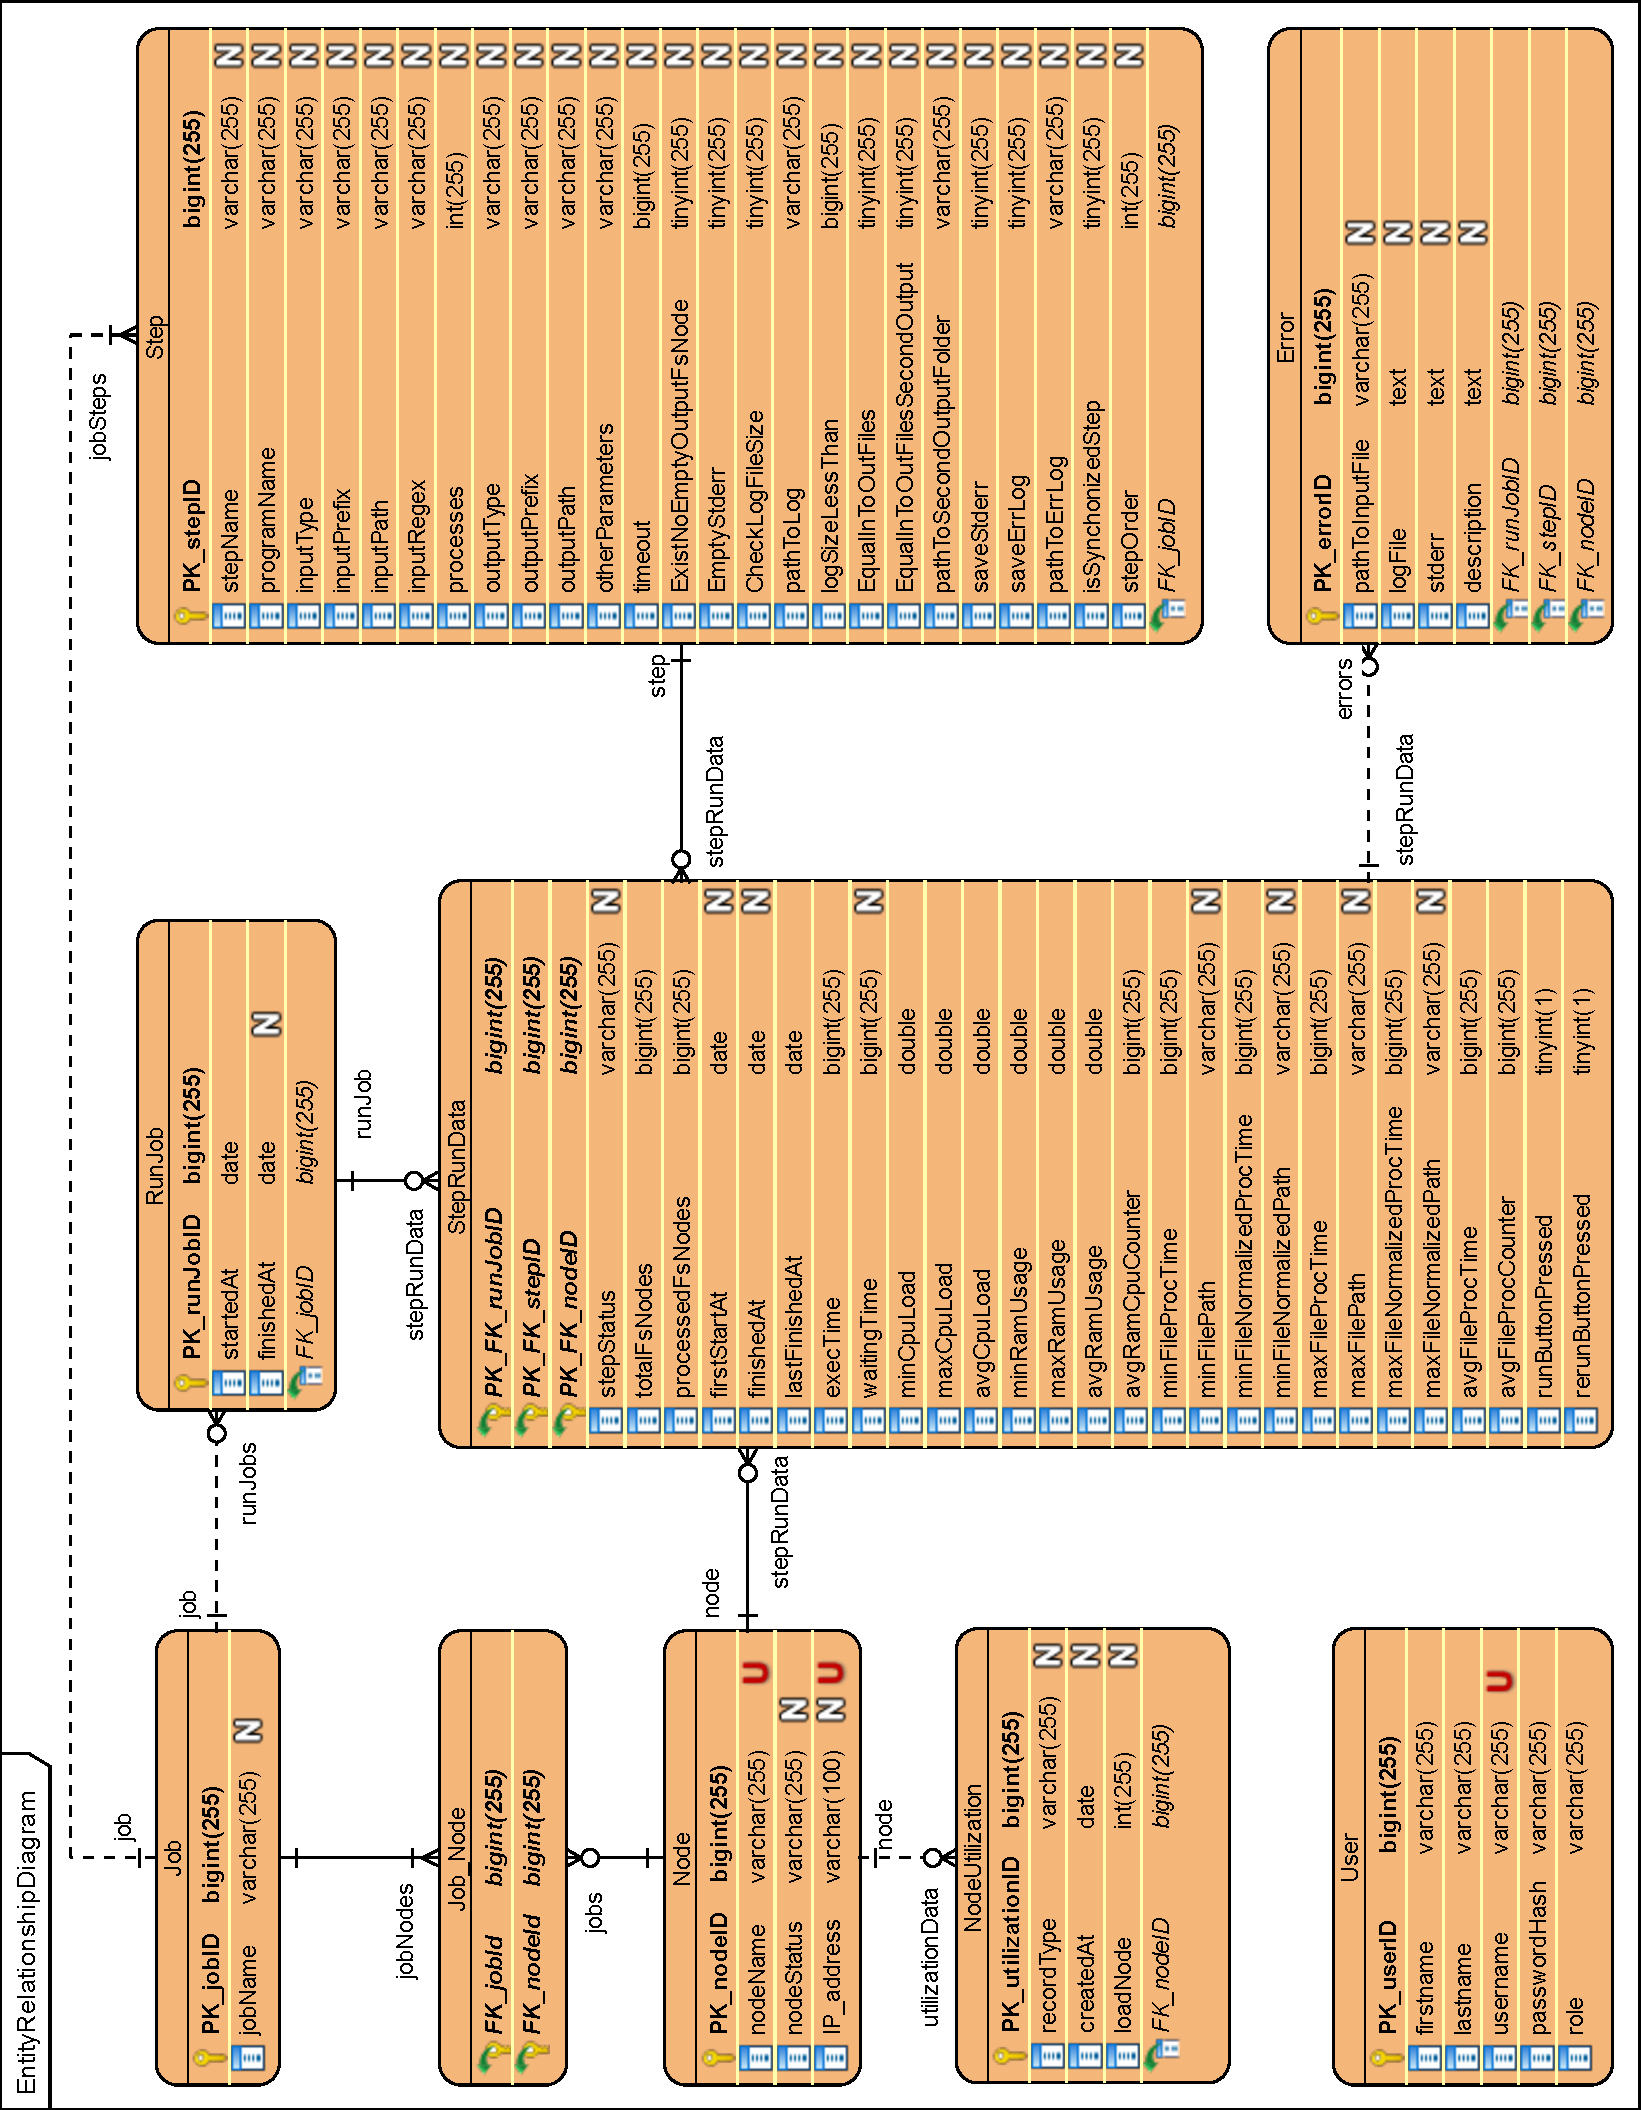
\includegraphics{images/EntityRelationshipDiagram.pdf}
    }
    \caption{\label{obr:ER_diagram} {\it Entity Relationship diagram znázorňující uložení dat v databázi.}}
\end{center}
\end{figure}

%-----------------------------------------------------------------------------------------------------------------

\section{Aplikace pro výpočetní uzel}
\label{section:secondaryNodeAppDesign}

Tato kapitola je věnována návrhu aplikace pro výpočetní uzel. Pro návrh byl využit diagram balíčků, který je možné vidět na obrázku \ref{obr:packageDiagramSecondaryNode}. Z diagramu je zřejmé, že aplikace pro výpočetní uzel bude rozdělena na 2 hlavní části. 

První bude obsahovat balíčky, které budou společné jak pro centrální, tak pro výpočetní uzel. Balíček \textit{eventLogger} bude obsahovat třídy pro vytvoření loggerů pro logování chyb, událostí a socketové komunikace. Balíček \textit{socketCommunicators} bude obsahovat abstraktní třídy pro přijímání a zasílání zpráv pomocí socketů. Posledním společným balíčkem je balíček \textit{socketMessages}, který bude obsahovat zprávy a data zasílaná mezi centrálním a~výpočetním uzlem.

Druhá část bude obsahovat balíčky specifické pro výpočetní uzel. Prvním z nich bude balíček \textit{secLoggers}, který bude obsahovat loggery pro logování událostí a chyb specifických pro výpočetní uzel. \textit{StepExecution} bude sloužit pro spuštění jednoho kroku úlohy, načtení vstupů, monitorování spuštěného kroku úlohy a získávání údajů o využití systémových prostředků. Dále bude obsahovat balíček \textit{secConnStatusMaintainer} zajišťující udržování stavu uzlu, který může být následující:

\begin{itemize}
    \item Čekání na navázání spojení,
    \item Úloha neběží,
    \item Úloha běží.
\end{itemize}

Balíček \textit{secSocketCommunicators} bude obsahovat třídy implementující abstraktní třídy z balíčku \textit{socketCommunicators}, které budou zajišťovat odesílání a příjem zpráv specifických pro výpočetní uzel. Balíček \textit{outputValidator} bude implementovat všechny validace výstupů popsané v kapitole \ref{section:validationDesign}. Balíček \textit{configuration} pak bude zajišťovat načtení a zpracování konfiguračního souboru. Základní vstupně/výstupní operace, jako je načtení obsahu souboru, vytvoření složky, kontrola existence dané složky atd. bude zabezpečovat balíček \textit{fileManager}. Popisy chyb, které mohou v průběhu načítání vstupních souborů nebo v průběhu validací výstupů nastat, budou obsaženy v balíčku \textit{errMessages}.

\begin{figure}[H]
\begin{center}
    \scalebox{0.5}
    {
        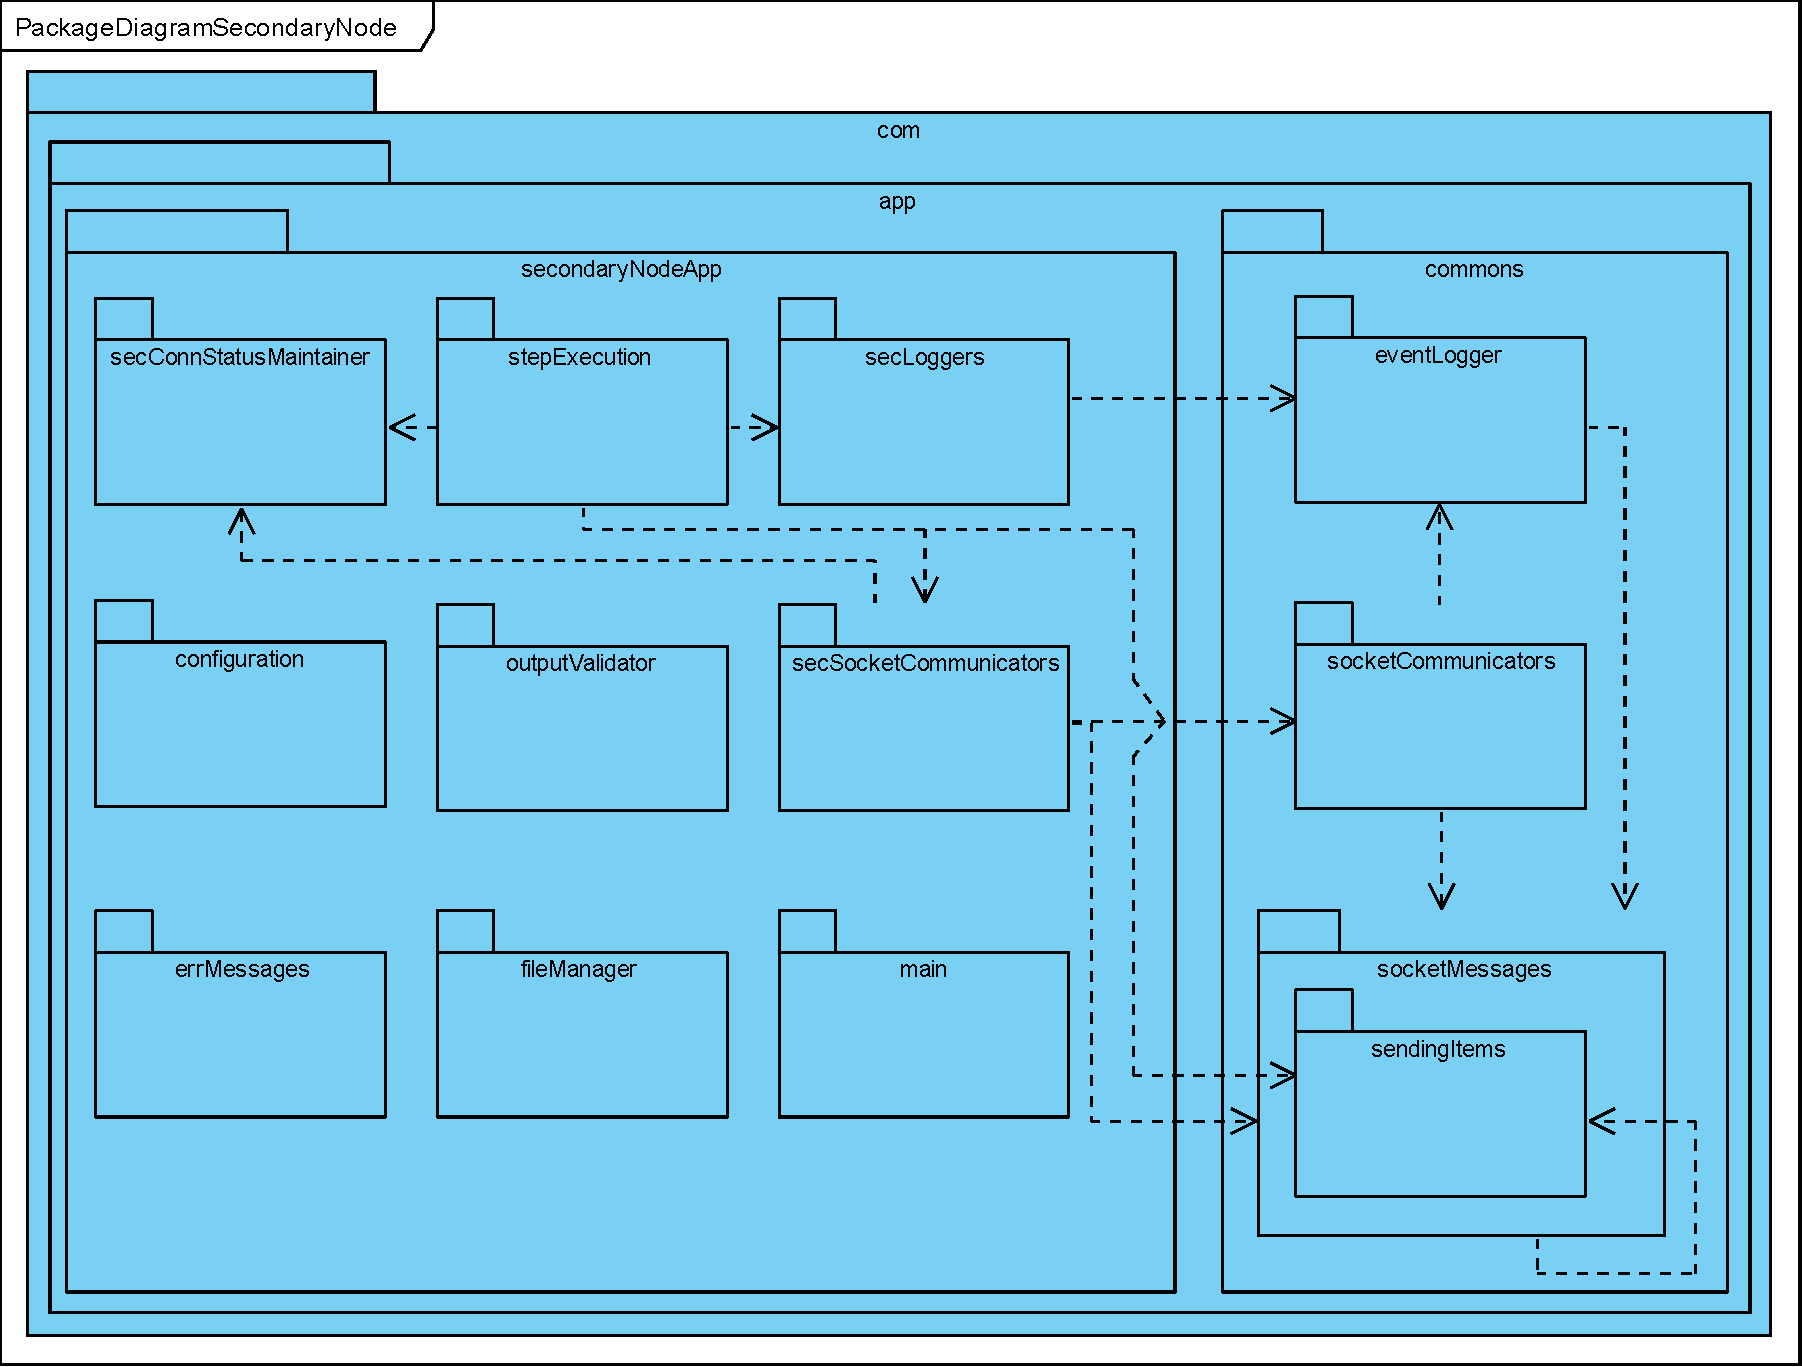
\includegraphics{images/PackageDiagramSecondaryNode.pdf}
    }
    \caption{\label{obr:packageDiagramSecondaryNode} {\it Diagram balíčků aplikace pro výpočetní uzel.}}
\end{center}
\end{figure}

\section{Aplikace pro centrální uzel}
\label{section:primaryNodeAppDesign}

V této podkapitole je popsán návrh aplikace pro centrální uzel. Aplikace bude založena na architektuře MVC. Nejnižší vrstva (Model), bude zajišťovat komunikaci s výpočetními uzly a s databází. Vrstva pohledu (View) bude reprezentována jednotlivými stránkami ve formátu XHTML, které budou popisovat vzhled aplikace. Prostřední vrstva (Controller) propojující vrstvy Model a~View bude realizována pomocí tzv. backing beanů. Ke každé stránce ve formátu XHTML bude vytvořen odpovídající backing bean. Tento backing bean bude určen ke zpracování událostí od uživatele a načítání zobrazovaných dat. Tato architektura bude dále rozšířena o servisní vrstvu. Pro návrh byl stejně jako v předchozí kapitole použit diagram balíčků. Jeho podobu bez vrstvy pohledu (View) je možné vidět na obrázku \ref{obr:packageDiagramPrimaryNode}. Z diagramu je zřejmé, že aplikace bude obsahovat balíček \textit{commons}, který je sdílený s~aplikací pro výpočetní uzel. Jeho detailní popis je uveden v kapitole \ref{section:secondaryNodeAppDesign}. Samotná aplikace bude rozdělena na 5 hlavních částí -- \textit{primLoggers}, \textit{exceptionHandler}, \textit{services}, \textit{model} a \textit{controllers}.

Balíček \textit{primLoggers} bude obsahovat loggery pro logování událostí a chyb specifických pro centrální uzel. Součástí bude rovněž logger zajišťující logování chyb, které mohou nastat při práci s databází. Balíček \textit{exceptionHandler} bude sloužit pro zachytávání a zpracování výjimek, které mohou nastat. V případě zachycení výjimky zajistí přesměrování uživatele na odpovídající chybovou stránku.

Balíček \textit{model} bude představovat, nejnižší vrstvu architektury MVC. Tento balíček bude rozdělen na 2 další balíčky -- \textit{primaryNode} a \textit{database}. První z nich bude obsahovat EJB Singleton bean, který bude dle návrhového vzoru Fasáda poskytovat rozhraní pro snadné řízení zpracování na výpočetních uzlech z jednotlivých backing beanů. Balíček \textit{usageChecker} bude určen pro monitorování využití jednotlivých výpočetních uzlů a bude tato data ukládat do databáze. \textit{SecNodeManager} bude určen pro udržování spojení a komunikaci se všemi výpočetními uzly. Zbylé 2 balíčky budou mít obdobnou funkci jako analogické balíčky v aplikaci pro výpočetní uzel -- \textit{primSocketCommunicators} bude zajišťovat odesílání a příjem zpráv specifických pro centrální uzel od jednoho výpočetního uzlu a~\textit{primConnStatusMaintainer} bude udržovat aktuální stav spojení s konkrétním výpočetním uzlem, přičemž stav spojení může být následující:

\begin{itemize}
    \item Čekání na potvrzení spuštění úlohy,
    \item Čekání na potvrzení pozastavení úlohy,
    \item Úloha běží,
    \item Úloha neběží.
\end{itemize}
Balíček \textit{database} bude obsahovat persistentní třídy pro ORM a výčtové typy korespondující s těmito persistentními třídami. V tomto balíčku budou dále zahrnuty  DAO (Data Access Object) objekty, které budou zajišťovat CRUD (Create-Read-Update-Delete) operace pro snadnou manipulaci s databázovými objekty.

Balíček \textit{services} bude obsahovat služby pro manipulaci s daty jednotlivých entit v systému. V této vrstvě budou pro načítání dat z databáze využity DAO objekty. Tyto služby budou dále implementovat logiku pro výpočet dalších údajů z takto načtených dat. Balíček \textit{dataClasses} bude obsahovat třídy reprezentující data, která budou zobrazována v prezentační vrstvě, tj. na jednotlivých stránkách aplikace. Rozhraní pro práci s těmito daty pak budou specifikována v balíčku \textit{interfaces}.

Balíček \textit{controllers} bude představovat prostřední vrstvu architektury MVC. Balíčky \textit{SortBean}, \textit{FilterBean} a \textit{PickListBean} budou zajišťovat řazení, filtrování a výběr dat ze seznamu libovolných dat implementujících odpovídající rozhraní z balíčku \textit{Interfaces}. Balíček \textit{AbstractBeans} bude obsahovat abstraktní beany, které budou implementovat společnou funkcionalitu pro více backing beanů. Pro každou stránku aplikace bude tento balíček dále obsahovat odpovídající controller, tj. backing bean, jak bylo uvedeno na začátku této kapitoly, kterým odpovídají zbývající balíčky.

\eject \pdfpagewidth=420mm
\begin{figure}[H]
    \scalebox{0.5 }
    {
        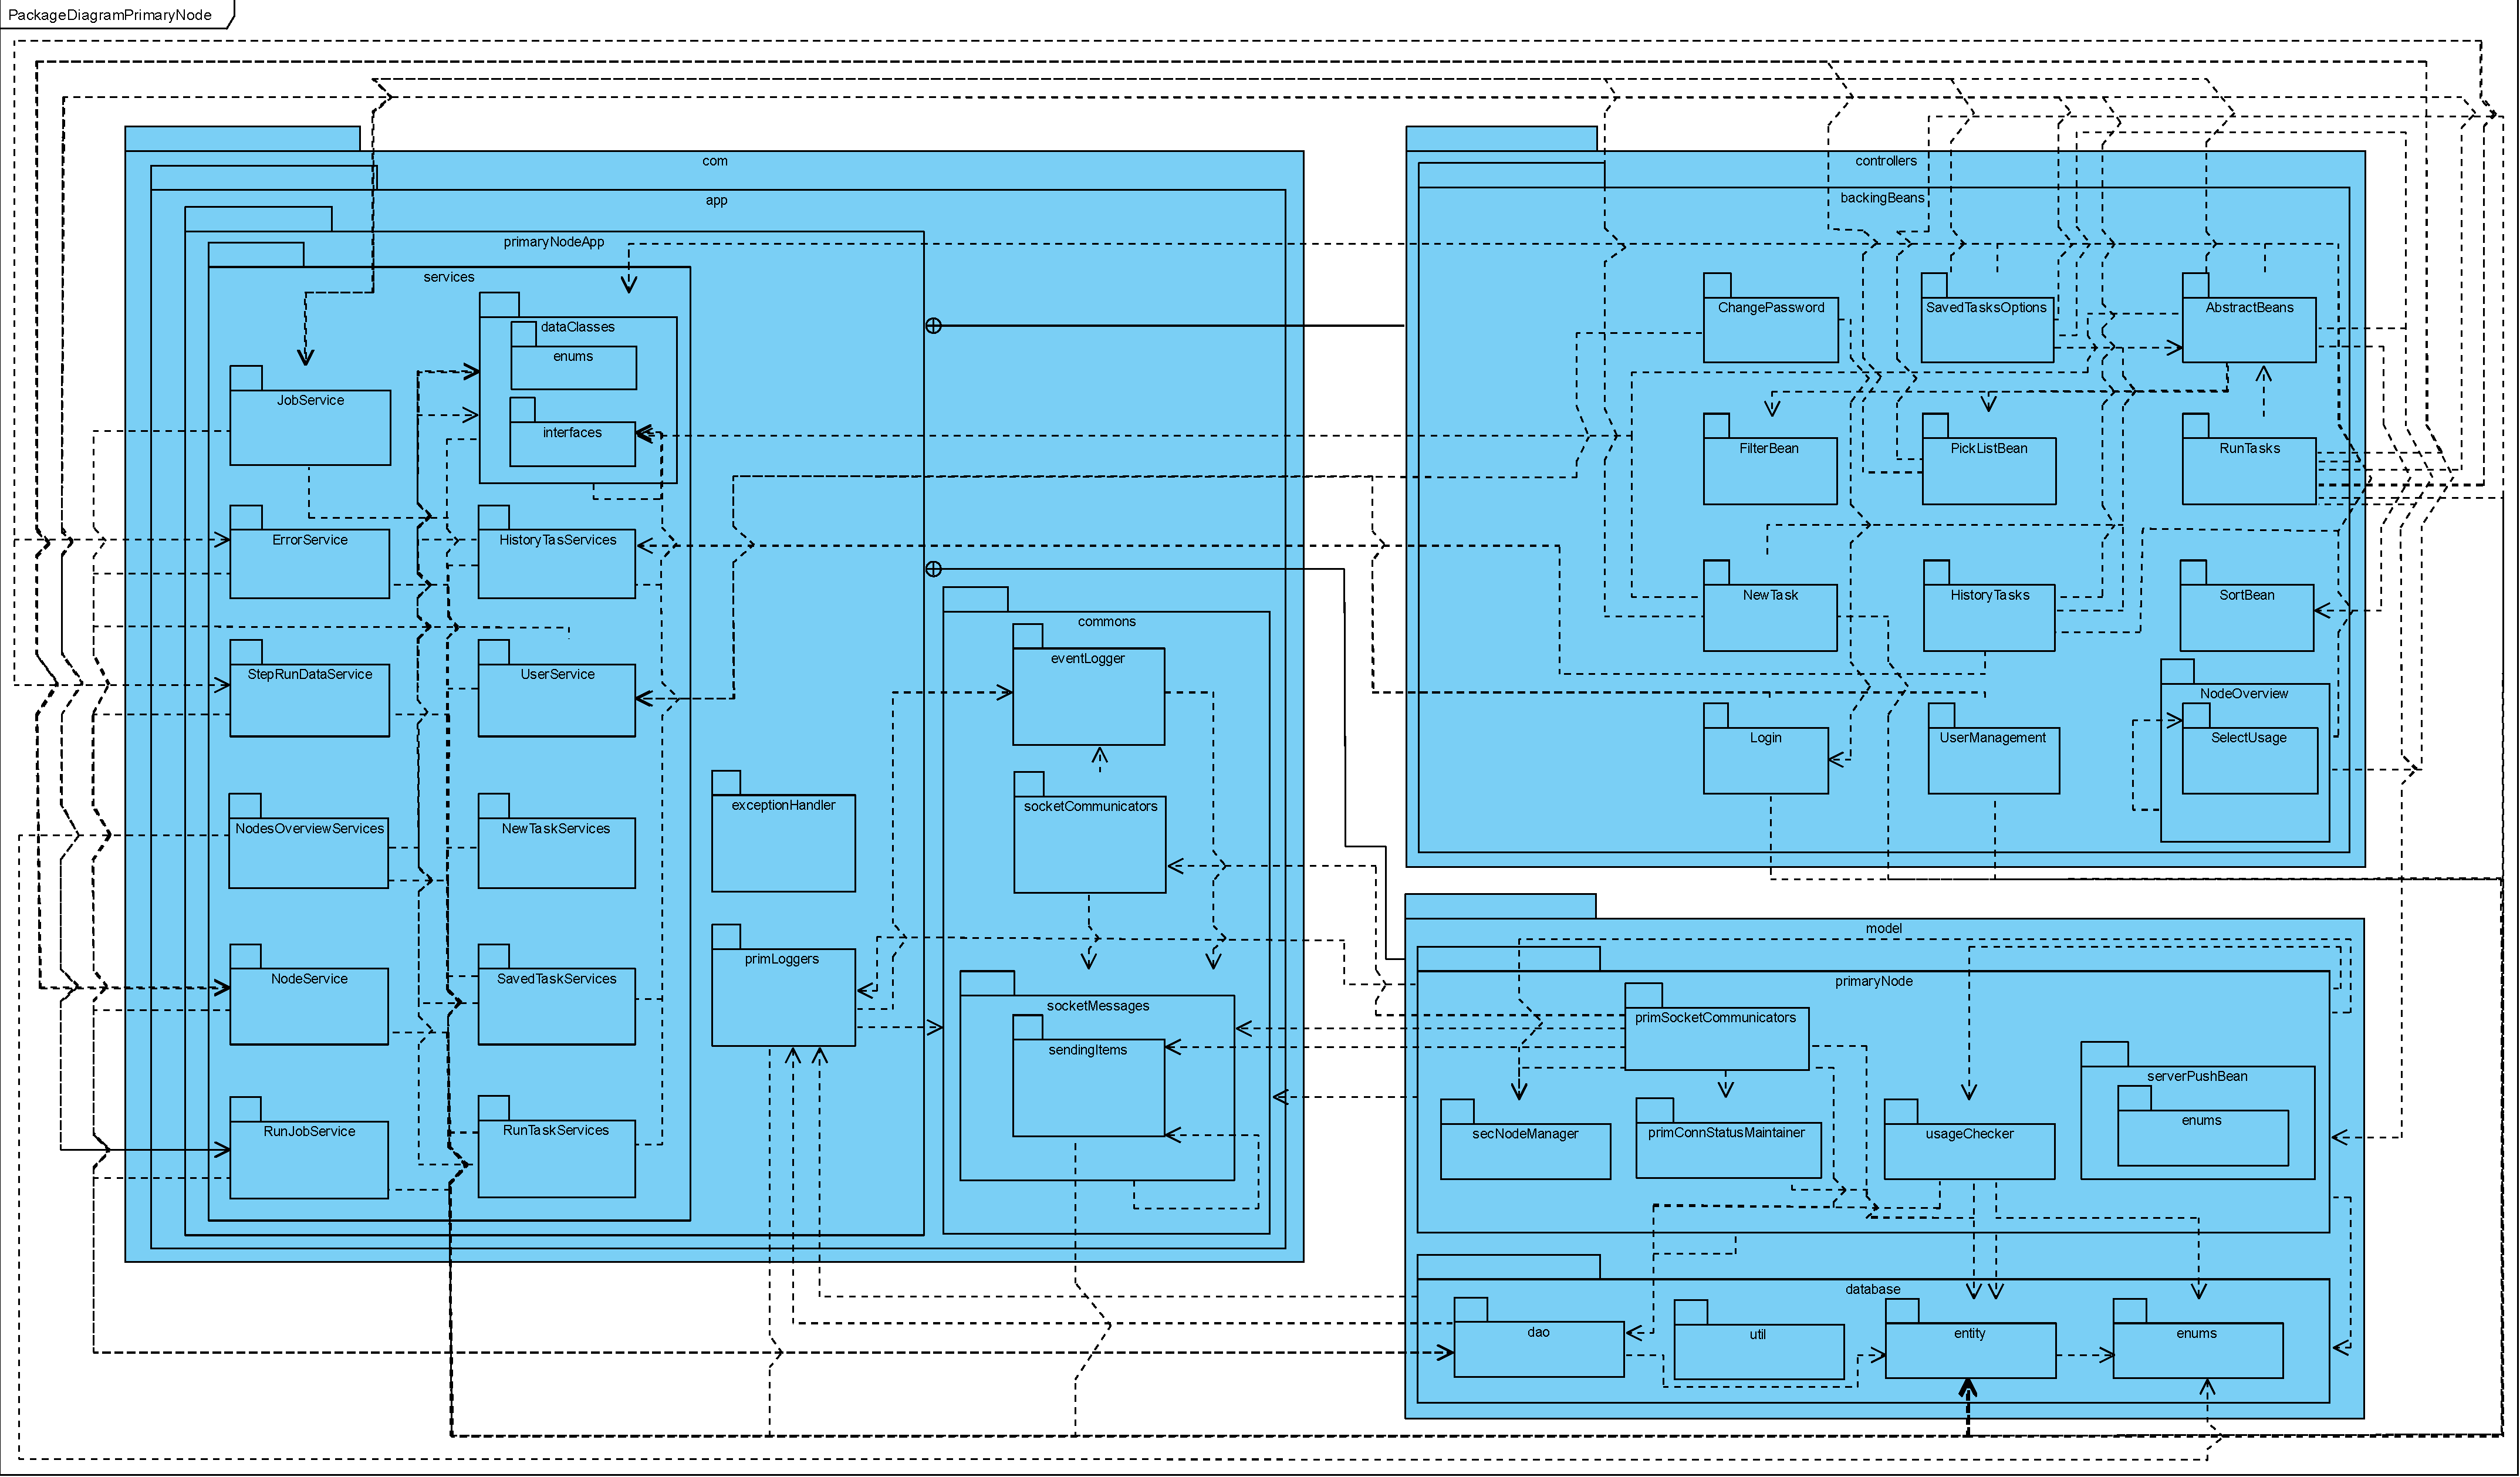
\includegraphics{images/PackageDiagramPrimaryNode.pdf}
    }
    \caption{\label{obr:packageDiagramPrimaryNode} {\it Diagram balíčků aplikace pro centrální uzel.}}
\end{figure}

\eject \pdfpagewidth=210mm

\section{Návrh komunikace centrálního uzlu s výpočetními uzly}
\label{section:communicationDesign}

Centrální uzel bude s jednotlivými výpočetními uzly komunikovat pomocí šifrovaného socketového spojení využívajícího protokol TCP/IP\footnote{https://tools.ietf.org/html/rfc1180} (Transmission Control Protocol/Internet Protocol). Výpočetní uzly se tedy budou k centrálnímu uzlu připojovat pomocí známé IP adresy a~portu. Diagram tříd pro jednotlivé typy zpráv a data, která budou během komunikace zasílána, je možné vidět na obrázku \ref{obr:classDiagramSocketMessages}. Z diagramu je zřejmé, že komunikace bude založena na 13 typech zpráv, jejichž význam je následující:

\begin{itemize}
    \item Zprávy zasílané z výpočetního uzlu na centrální uzel:
        \begin{itemize}
            \item \textit{NodeNameMsg} -- zpráva oznamující centrálnímu uzlu jméno připojovaného výpočetního uzlu,
            \item \textit{RunStepAckMsg} -- zpráva potvrzující spuštění kroku úlohy, obsahuje informaci o počtu vstupů,
            \item \textit{StopStepAckMsg} -- zpráva potvrzující úspěšné pozastavení kroku úlohy,
            \item \textit{RerunAckMsg} -- zpráva potvrzující úspěšné spuštění opětovného zpracování chybných vstupů,
            \item \textit{ProcFinishedMsg} -- zpráva oznamující úspěšné dokončení zpracování konkrétního vstupu daného kroku úlohy,
            \item \textit{ProcErrorMsg} -- zpráva oznamující neúspěšné zpracování konkrétního kroku úlohy,
            \item \textit{UsageMsg} -- zpráva obsahující informace o využití systémových prostředků, která je periodicky zasílána v případě běžícího kroku úlohy.
        \end{itemize}
    \item Zprávy zasílané z centrálního uzlu na výpočetní uzly:
        \begin{itemize}
            \item \textit{AcceptConnMsg} -- zpráva oznamující výpočetnímu uzlu akceptaci spojení,
            \item \textit{DeclineConnMsg} -- zpráva oznamující výpočetnímu uzlu odmítnutí spojení,
            \item \textit{RunStepMsg} -- zpráva obsahující požadavek na spuštění konkrétního kroku úlohy,
            \item \textit{StopStepMsg} -- zpráva obsahující požadavek na pozastavení provádění spuštěného kroků úlohy,
            \item \textit{RerunMsg} -- zpráva obsahující požadavek na opětovné spuštění chybných vstupů.
        \end{itemize}
    \item Zprávy zasílané jak z centrálního, tak z výpočetních uzlů:
        \begin{itemize}
            \item \textit{isAliveMsg} -- zpráva, která bude periodicky zasílána protistraně s cílem ověřit, zda je spojení stále aktivní.
        \end{itemize}
\end{itemize}

\begin{figure}[H]
\begin{center}
    \scalebox{0.5}
    {
        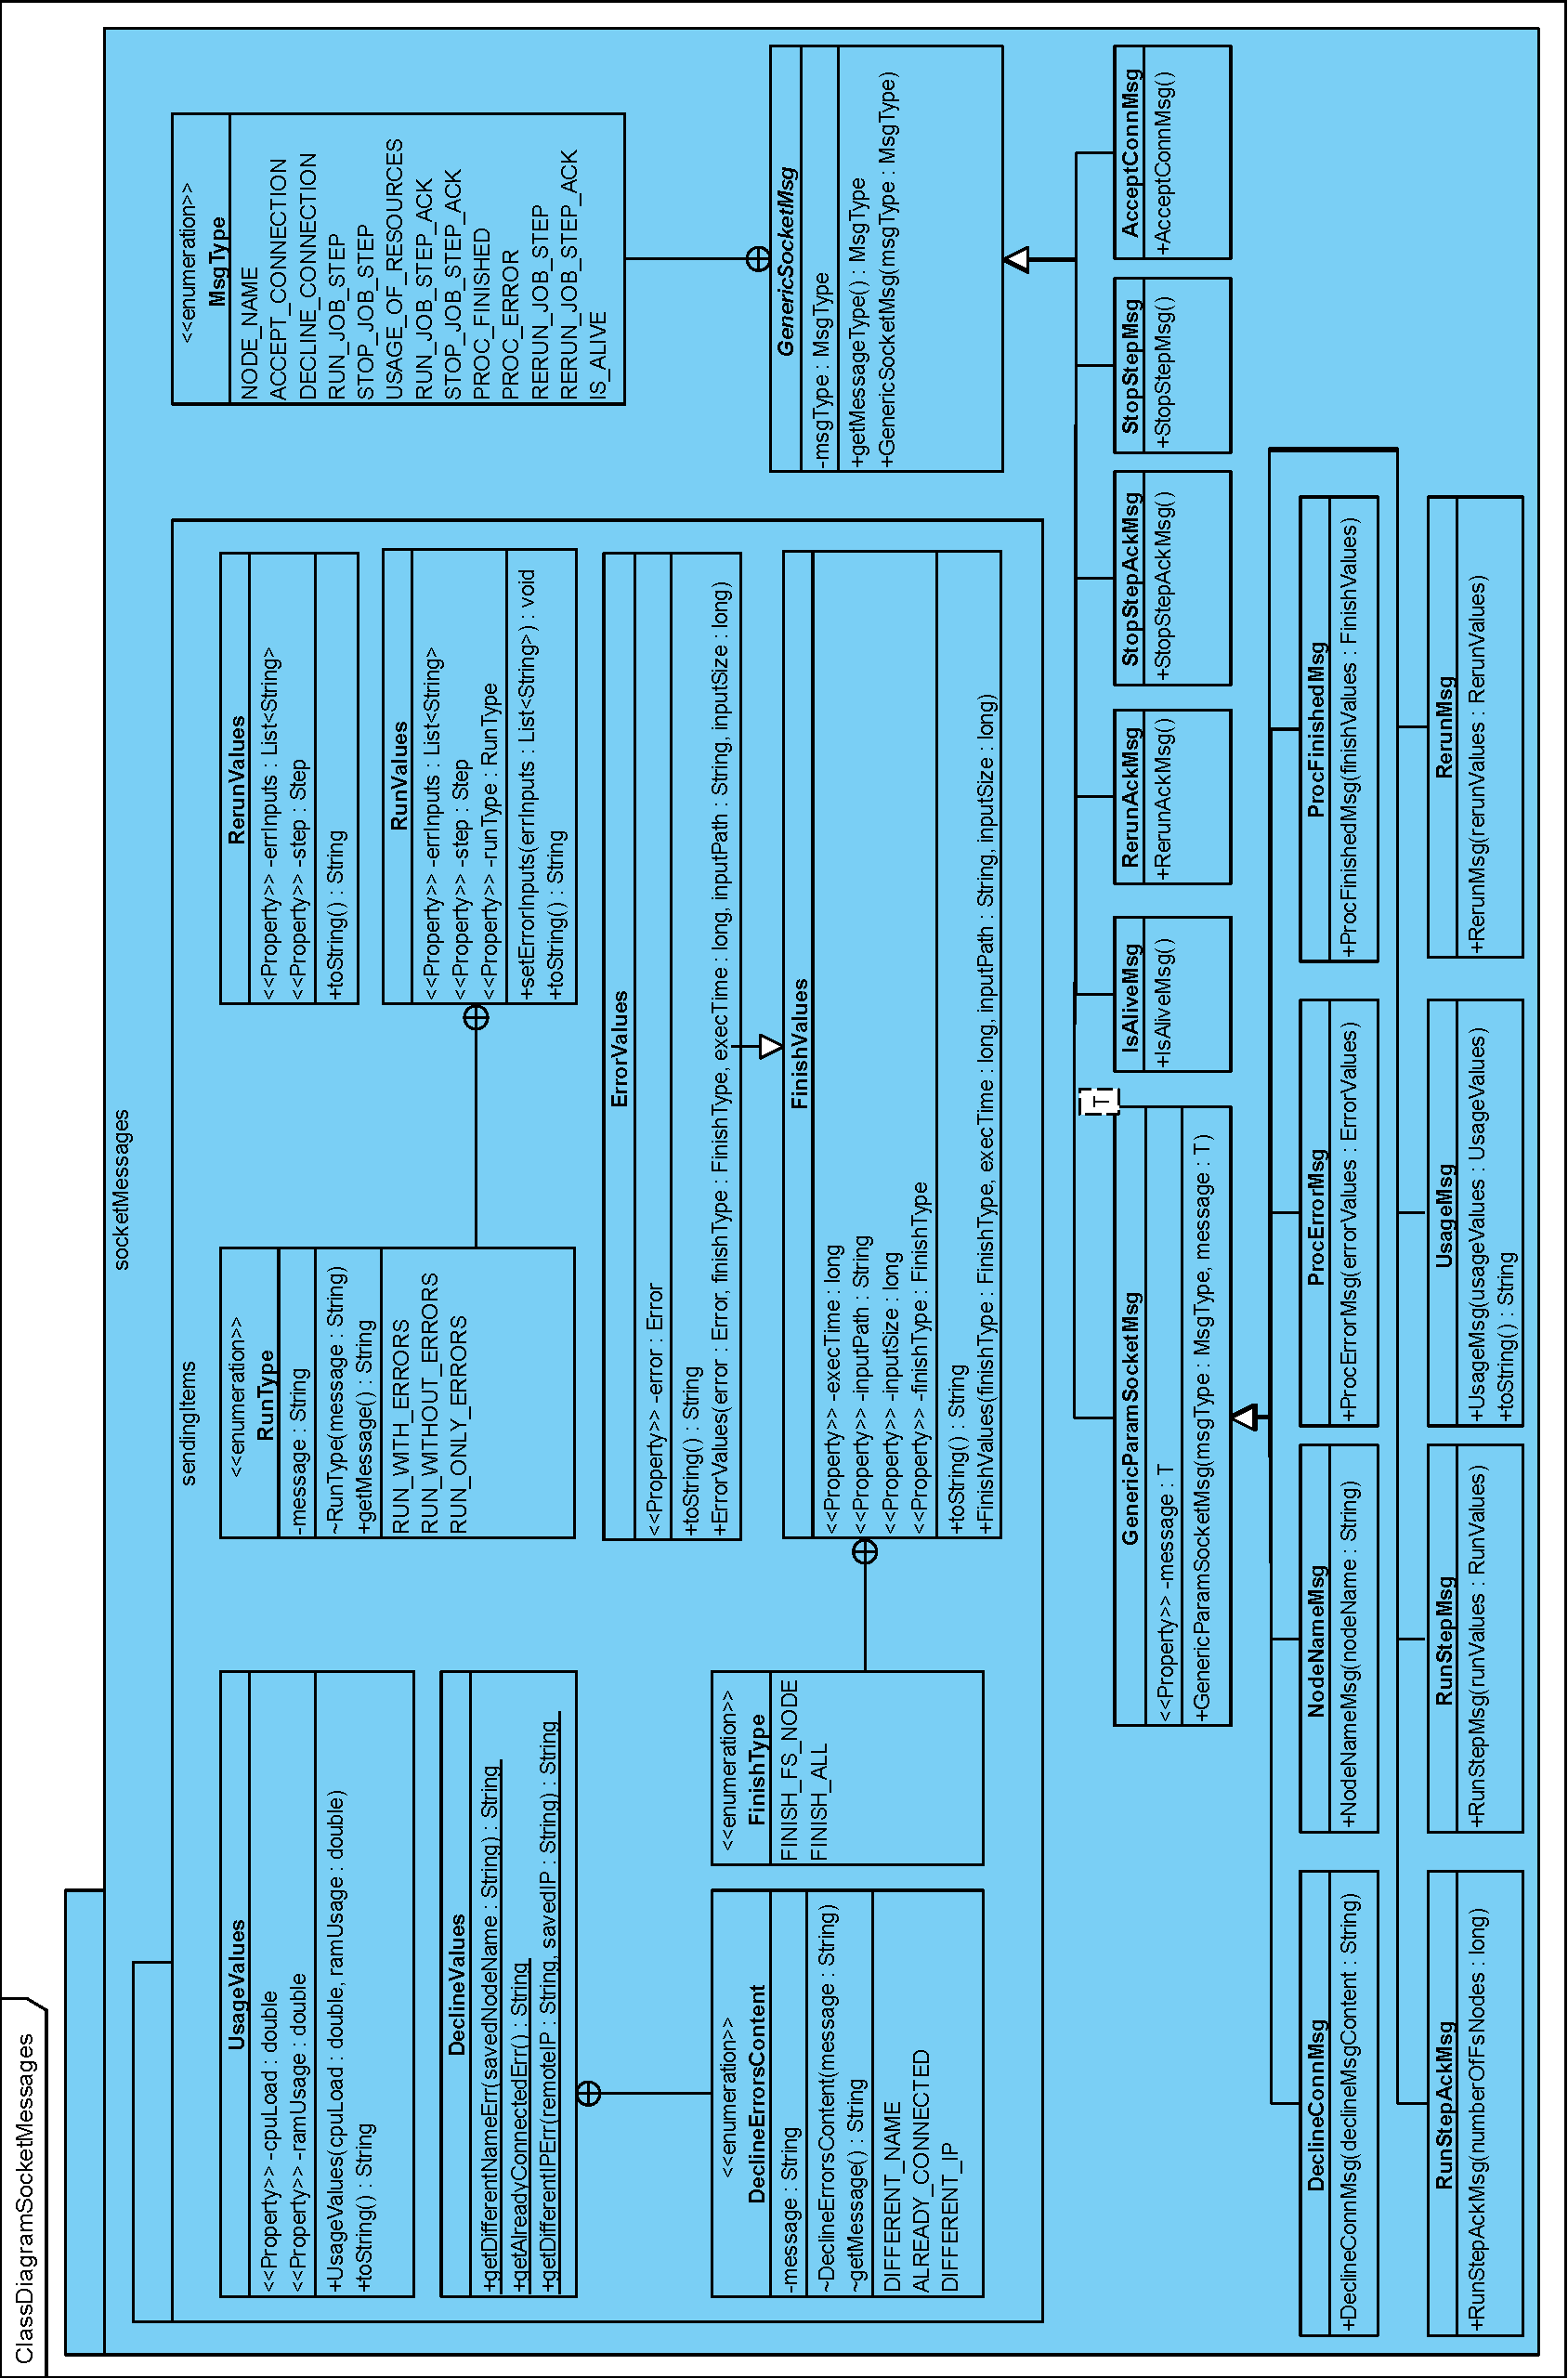
\includegraphics{images/ClassDiagramSocketMessages.pdf}
    }
    \caption{\label{obr:classDiagramSocketMessages} {\it Diagram tříd znázorňující zprávy a data zasílaná mezi centrálním a výpočetním uzlem.}}
\end{center}
\end{figure}

V balíčku \textit{sendingItems} budou specifikována data, která budou v rámci zpráv přenášena. Třída \textit{UsageValues} bude obsahovat data o využití systémových prostředků, která budou zasílána v rámci zprávy \textit{UsageMsg}. Třída \textit{DeclineValues} bude definovat příčiny odmítnutí spojení s daným výpočetním uzlem. \textit{RerunValues} bude obsahovat data, která budou zasílána v rámci zprávy \textit{RerunMsg}. Bude obsahovat popis kroku úlohy, u nějž má být zpracování chybných vstupů opětovně spuštěno, a seznam těchto chybných vstupů. Třída \textit{RunValues} bude obsahovat stejné informace, avšak navíc bude obsahovat informaci o typu spuštění, který může být následující:

\begin{itemize}
    \item \textit{RUN\_WITH\_ERRORS} -- v rámci daného kroku úlohy budou zpracovány všechny nezpracované vstupy včetně vstupů, které skončily s chybou, přičemž chybové vstupy budou zpracovány jako první,
    \item \textit{RUN\_WITHOUT\_ERRORS} -- v rámci daného kroku úlohy budou zpracovány všechny nezpracované vstupy, přičemž chybové vstupy budou ze zpracování vynechány,
    \item \textit{RUN\_ONLY\_ERRORS} -- v rámci daného kroku budou zpracovány pouze chybové vstupy.
\end{itemize}

\textit{FinishValues} bude nést informaci o celkové době zpracování daného vstupu a typu ukončovací zprávy, který závisí na tom, zda na daném výpočetním uzlu existují nějaké nezpracované vstupy nebo zda se jedná o poslední zpracovaný vstup. Tyto informace budou zasílány v rámci zpráv \textit{ProcFinishedMsg} a \textit{ProcErrorMsg}. Třída \textit{ErrorValues} bude pracovat s identickými daty jako třída \textit{FinishedValues}, avšak oproti ní bude navíc obsahovat údaje o~chybě, která nastala, včetně obsahu logu, případně standardního chybového výstupu (v~závislosti na konfiguraci daného kroku úlohy). Tento typ dat bude zasílán v rámci zprávy \textit{ProcErrorMsg}.

\subsection*{Navázání spojení výpočetního a centrálního uzlu}

Sekvenční diagram znázorňující navazování spojení na výpočetním uzlu je možné vidět na obrázku \ref{obr:sequenceDiagramEstablishingOfConnectionSecondaryNode}. Výpočetní uzel zašle po navázání socketového spojení na centrální uzel zprávu \textit{NodeNameMsg}, která bude obsahovat jeho jméno. Dle typu odpovědi buď vypíše chybu, která během navazování spojení nastala, a ukončí jej nebo začne v pravidelných intervalech odesílat zprávy typu \textit{IsAliveMsg}.

\begin{figure}[H]
\begin{center}
    \scalebox{0.5}
    {
        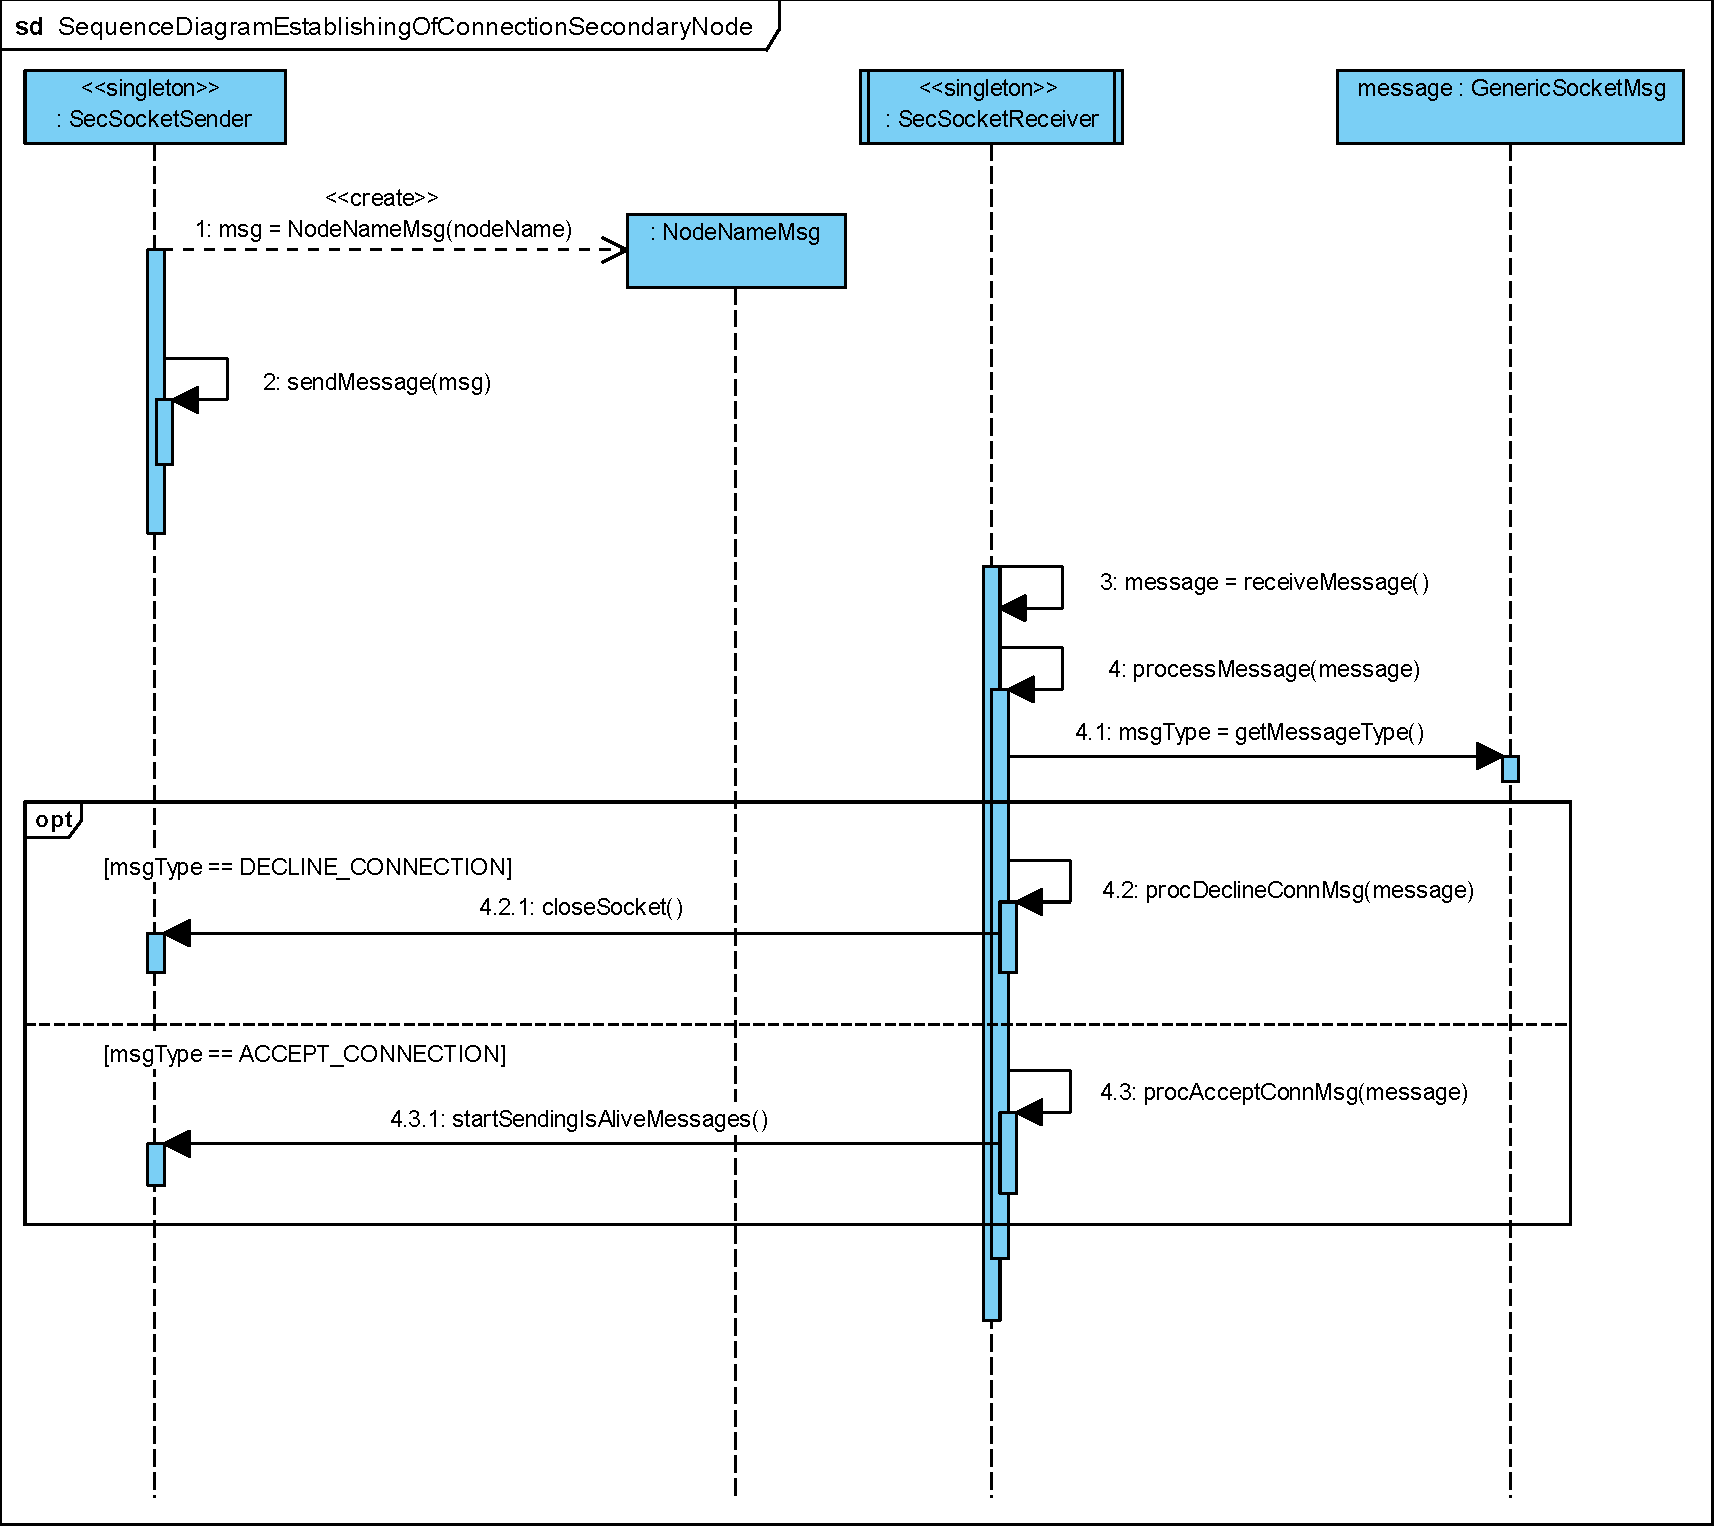
\includegraphics{images/SequenceDiagramEstablishingOfConnectionSecondaryNode.pdf}
    }
    \caption{\label{obr:sequenceDiagramEstablishingOfConnectionSecondaryNode} {\it Sekvenční diagram znázorňující navázání spojení na výpočetním uzlu.}}
\end{center}
\end{figure}

Na obrázku \ref{obr:sequenceDiagramEstablishingOfConnectionPrimaryNode} je možné vidět proces navazování spojení z pohledu centrálního uzlu. Z~diagramu je zřejmé, že pokud se výpočetní uzel bude připojovat k centrálnímu uzlu poprvé, budou informace o daném výpočetním uzlu uloženy do databáze. V opačném případě bude nejprve ze stavu uzlu ověřeno, zda není uzel s přijatým jménem již připojen (aplikace centrálního uzlu bude předpokládat unikátnost názvu každého výpočetního uzlu) a~zda se výpočetní uzel připojuje ze stejné IP adresy. Pokud bude některá z podmínek porušena, bude na výpočetní uzel odeslána zpráva \textit{DeclineConnMsg} a spojení bude ukončeno. V opačném případě bude na výpočetní uzel odeslána zpráva \textit{AcceptConnMsg}. Poté bude na výpočetní uzel v pravidelných intervalech odesílána zpráva \textit{IsAliveMsg}. Po úspěšném navázání spojení budou postupně odesílány ke zpracování všechny nezpracované kroky rozpracovaných úloh.

\begin{figure}[H]
\begin{center}
    \scalebox{0.5}
    {
        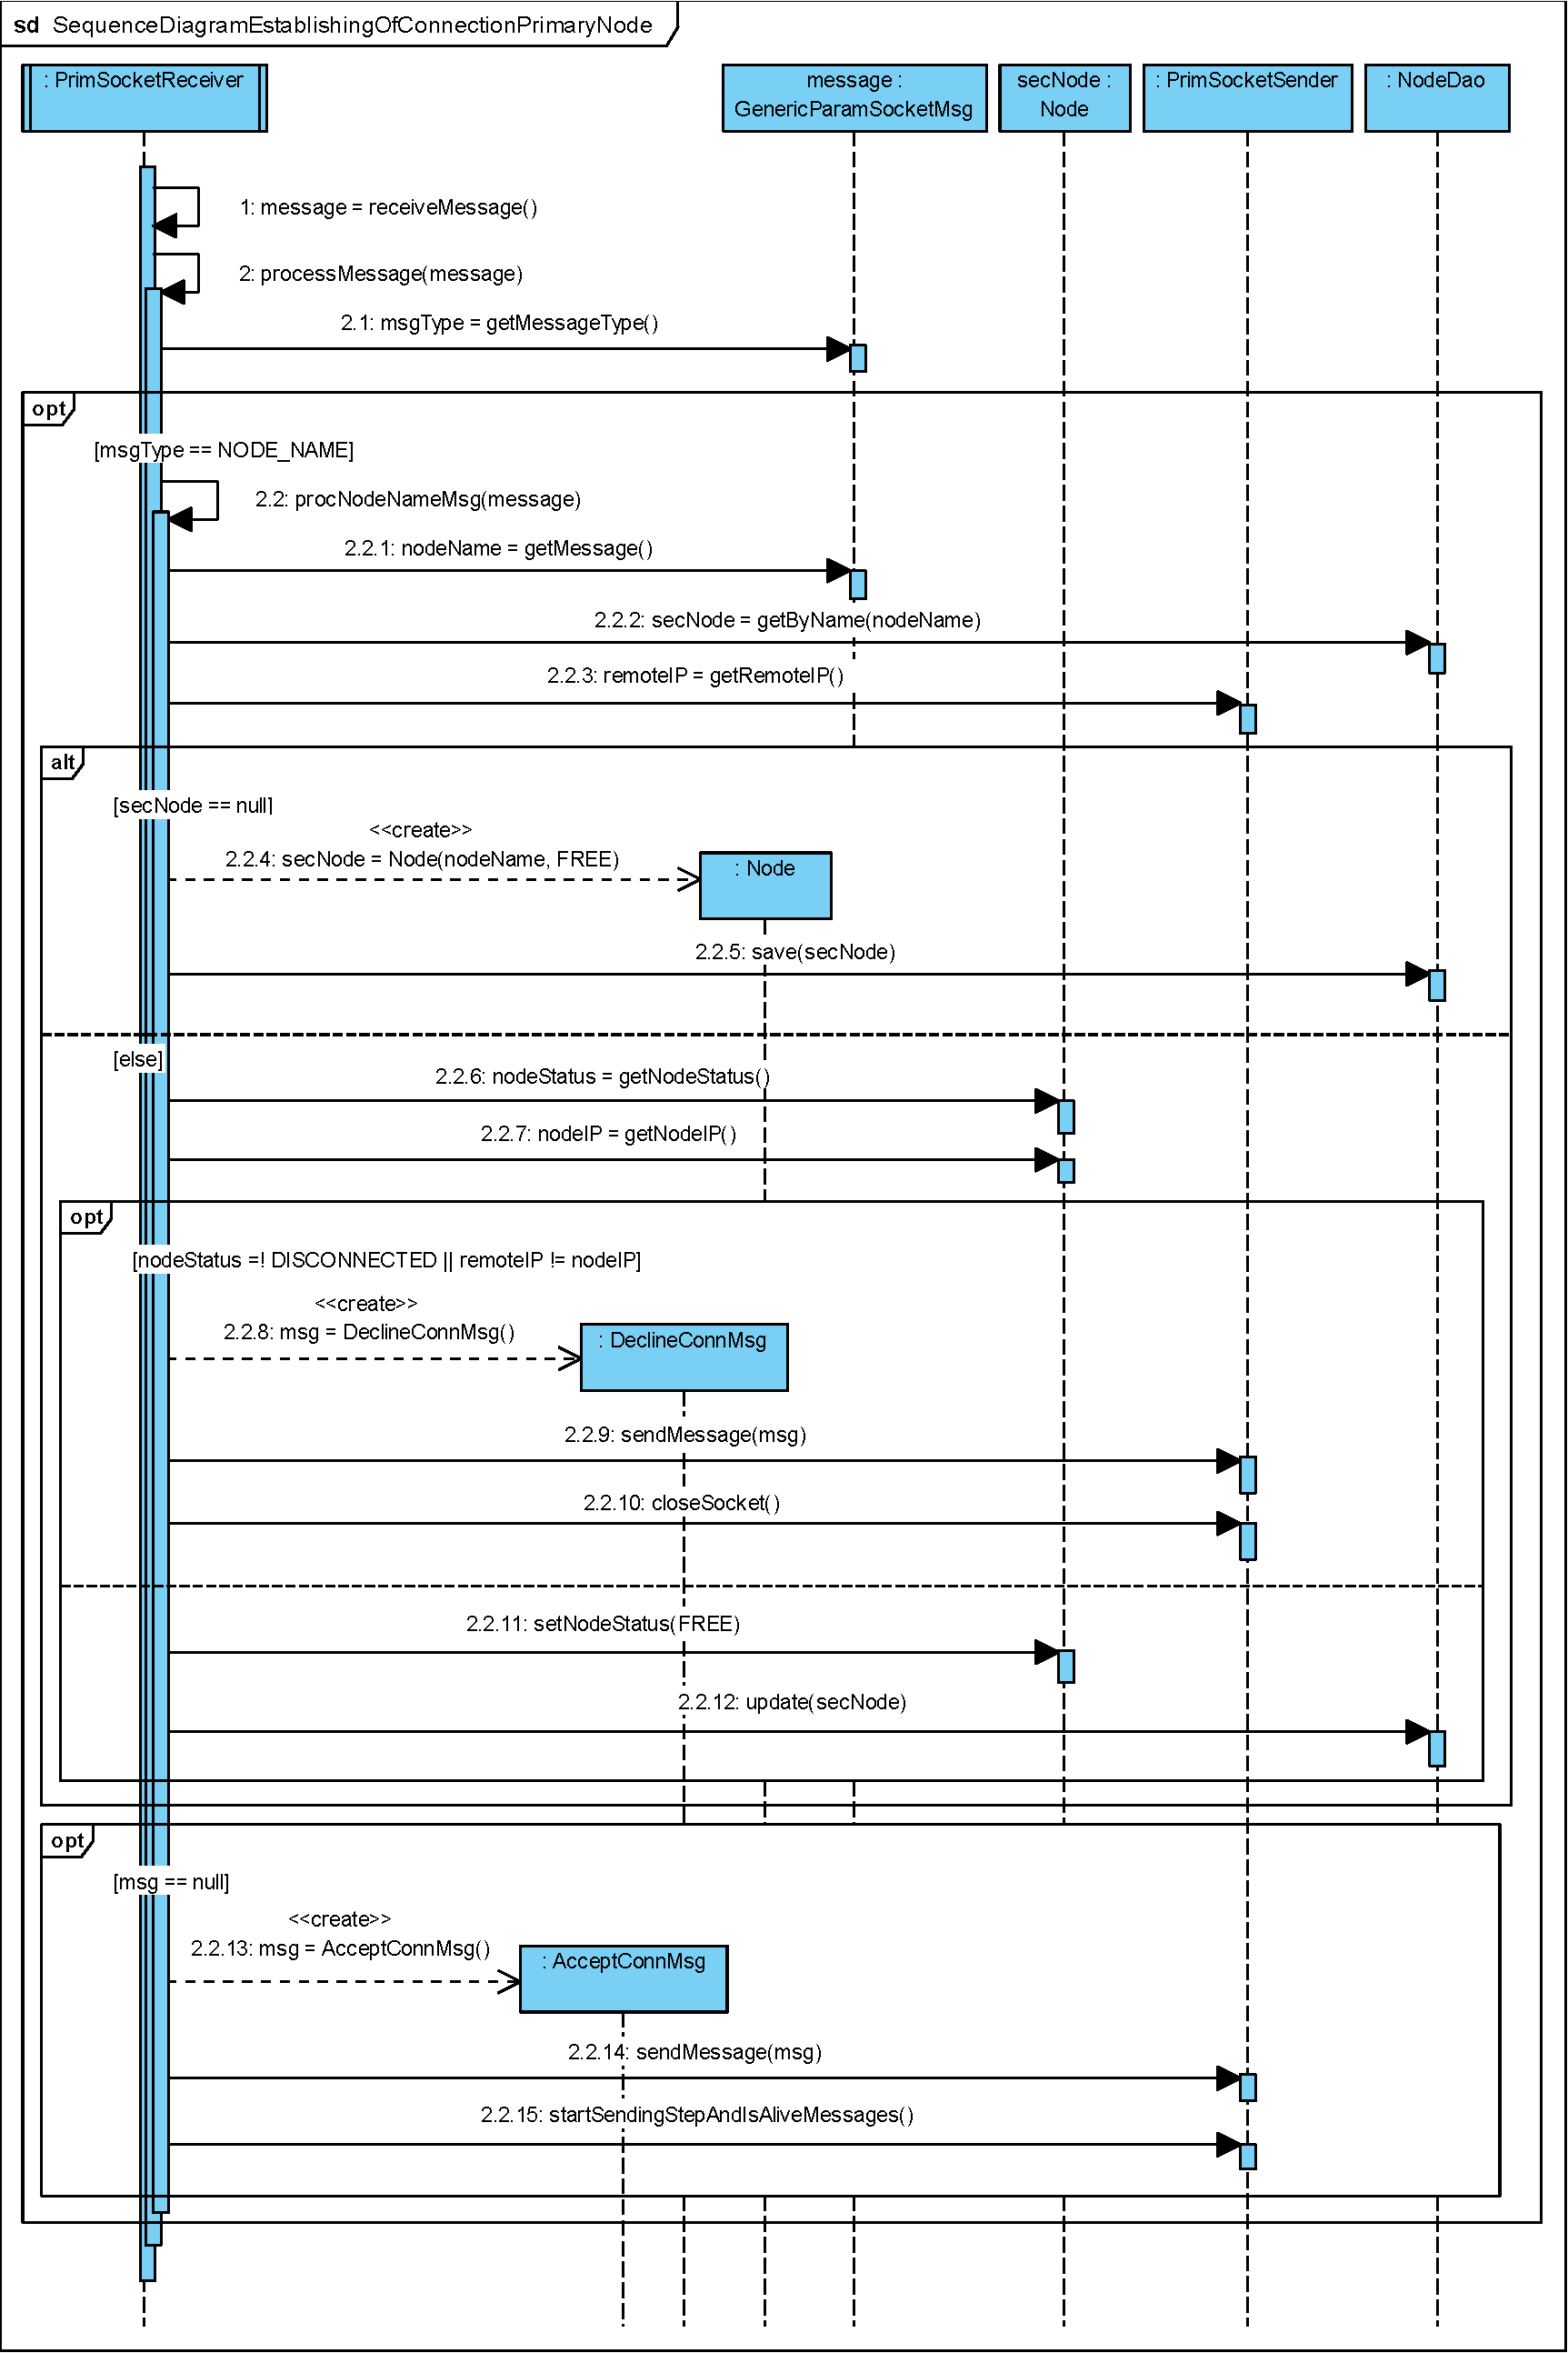
\includegraphics{images/SequenceDiagramEstablishingOfConnectionPrimaryNode.pdf}
    }
    \caption{\label{obr:sequenceDiagramEstablishingOfConnectionPrimaryNode} {\it Sekvenční diagram znázorňující navázání spojení na centrálním uzlu}}
\end{center}
\end{figure}

\section{Spuštění zpracování úlohy}
\label{section:RunTask}

\subsection*{Spuštění úlohy na centrálním uzlu}
\label{subsection:RunTaskOnPrimaryNode}

Průběh zpracování požadavku na vytvoření a spouštění nové úlohy je zobrazen na obrázku~\ref{obr:sequenceDiagramRunTaskPrimaryNode}. Po přijetí požadavku typu POST bude zavolána odpovídající metoda backing beanu. V této metodě budou nejprve ze zadaných údajů získána data o~jednotlivých krocích úlohy vhodná pro uložení do databáze -- bude nutné provést konverzi zadaných hodnot tak, aby byla tato data ukládána ve stejných jednotkách. Z odpovídajícího backing beanu bude dále získán seznam uzlů, na kterých má být úloha spuštěna. Tato data budou následně uložena do databáze. Zároveň bude vytvořen a uložen nový běh úlohy, čímž dojde k~implicitnímu zařazení prvního kroku úlohy do fronty proveditelných kroků u~každého výpočetního uzlu, jelikož budou po úspěšném navázání spojení proveditelné kroky postupně načítány z databáze a vykonávány v pořadí od nejstaršího po nejnovější, jak je uvedeno v~kapitole \ref{section:communicationDesign}. Jakmile budou všechny proveditelné kroky dokončeny, nebude dále docházet k periodické kontrole přítomnosti nového proveditelného kroku v databázi, jelikož by to znamenalo její zbytečné zatěžování. Z této skutečnosti vyplývá, že při vytvoření nové úlohy bude nutné zajistit u všech odesílatelů kroků na volné připojené uzly načtení a odeslání nového proveditelného kroku. Toto bude zajištěno změnou odpovídajícího příznaku u objektu \textit{PrimConnStatusMaintainer}, který bude udržovat stav spojení s~konkrétním výpočetním uzlem. Za tímto účelem budou údaje o uložené úloze předány EJB beanu \textit{PrimaryNode}. Ten předá požadavek na změnu příznaku u odpovídajících odesílatelů na objekt \textit{SecNodeManager}, který bude zajišťovat komunikaci se všemi výpočetními uzly. 

Zpracování požadavku objektem \textit{SecNodeManager} je pro přehlednost umístěno v samostatném diagramu na obrázku \ref{obr:sequenceDiagramRunTaskPrimaryNodeSenderChangeFlag}. Komunikace s konkrétním výpočetním uzlem bude realizována objektem \textit{SecNodeCommunicator}, který bude obsahovat objekty pro příjem zprávy, odeslání zprávy a objekt obsahující stav spojení s konkrétním výpočetním uzlem. Změnou odpovídajícího příznaku provede odesílatel kroků na daný výpočetní uzel opětovnou kontrolu existence proveditelného kroku v databázi. Tím dojde k načtení prvního kroku nové úlohy a jeho odeslání ke zpracování na daný výpočetní uzel.

\begin{figure}[H]
\begin{center}
    \scalebox{0.5}
    {
        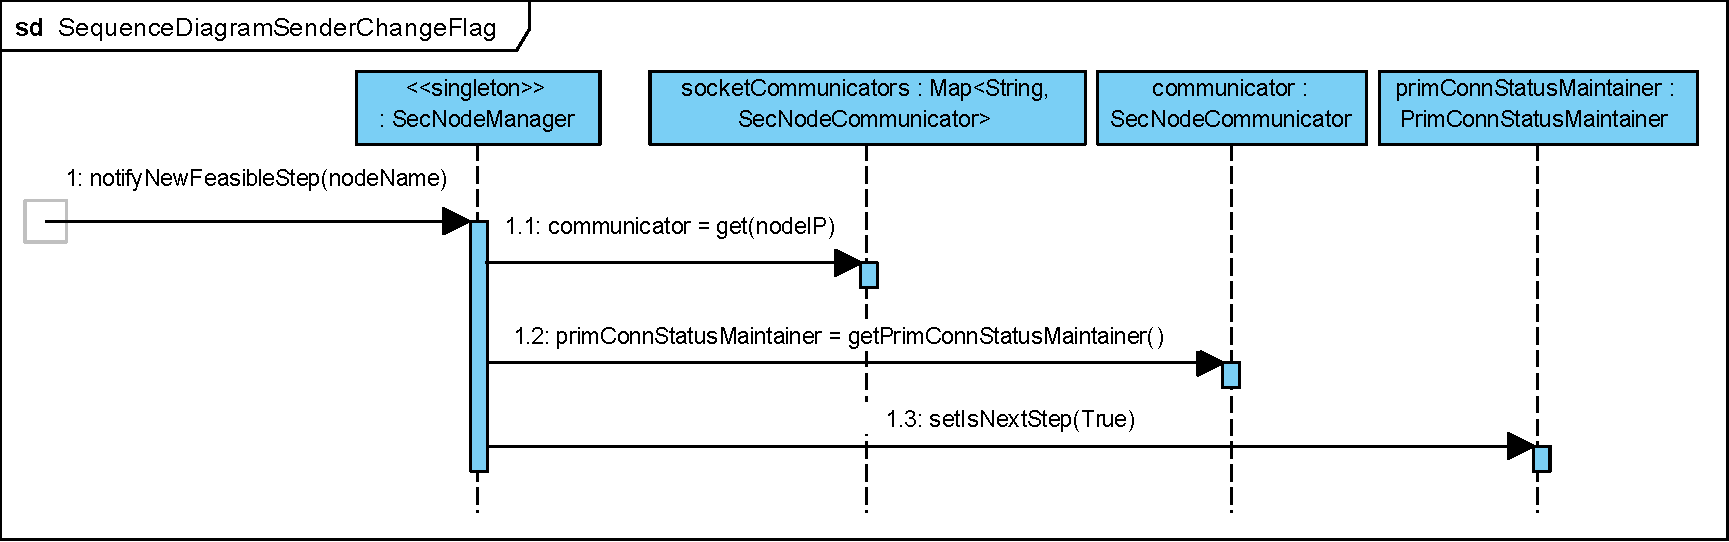
\includegraphics{images/SequenceDiagramSenderChangeFlag.pdf}
    }
    \caption{\label{obr:sequenceDiagramRunTaskPrimaryNodeSenderChangeFlag} {\it Sekvenční diagram znázorňující nastavení příznaku u odesílatele nezpracovaných kroků na výpočetní uzel.}}
\end{center}
\end{figure}

\begin{figure}[H]
\begin{center}
    \scalebox{0.5}
    {
        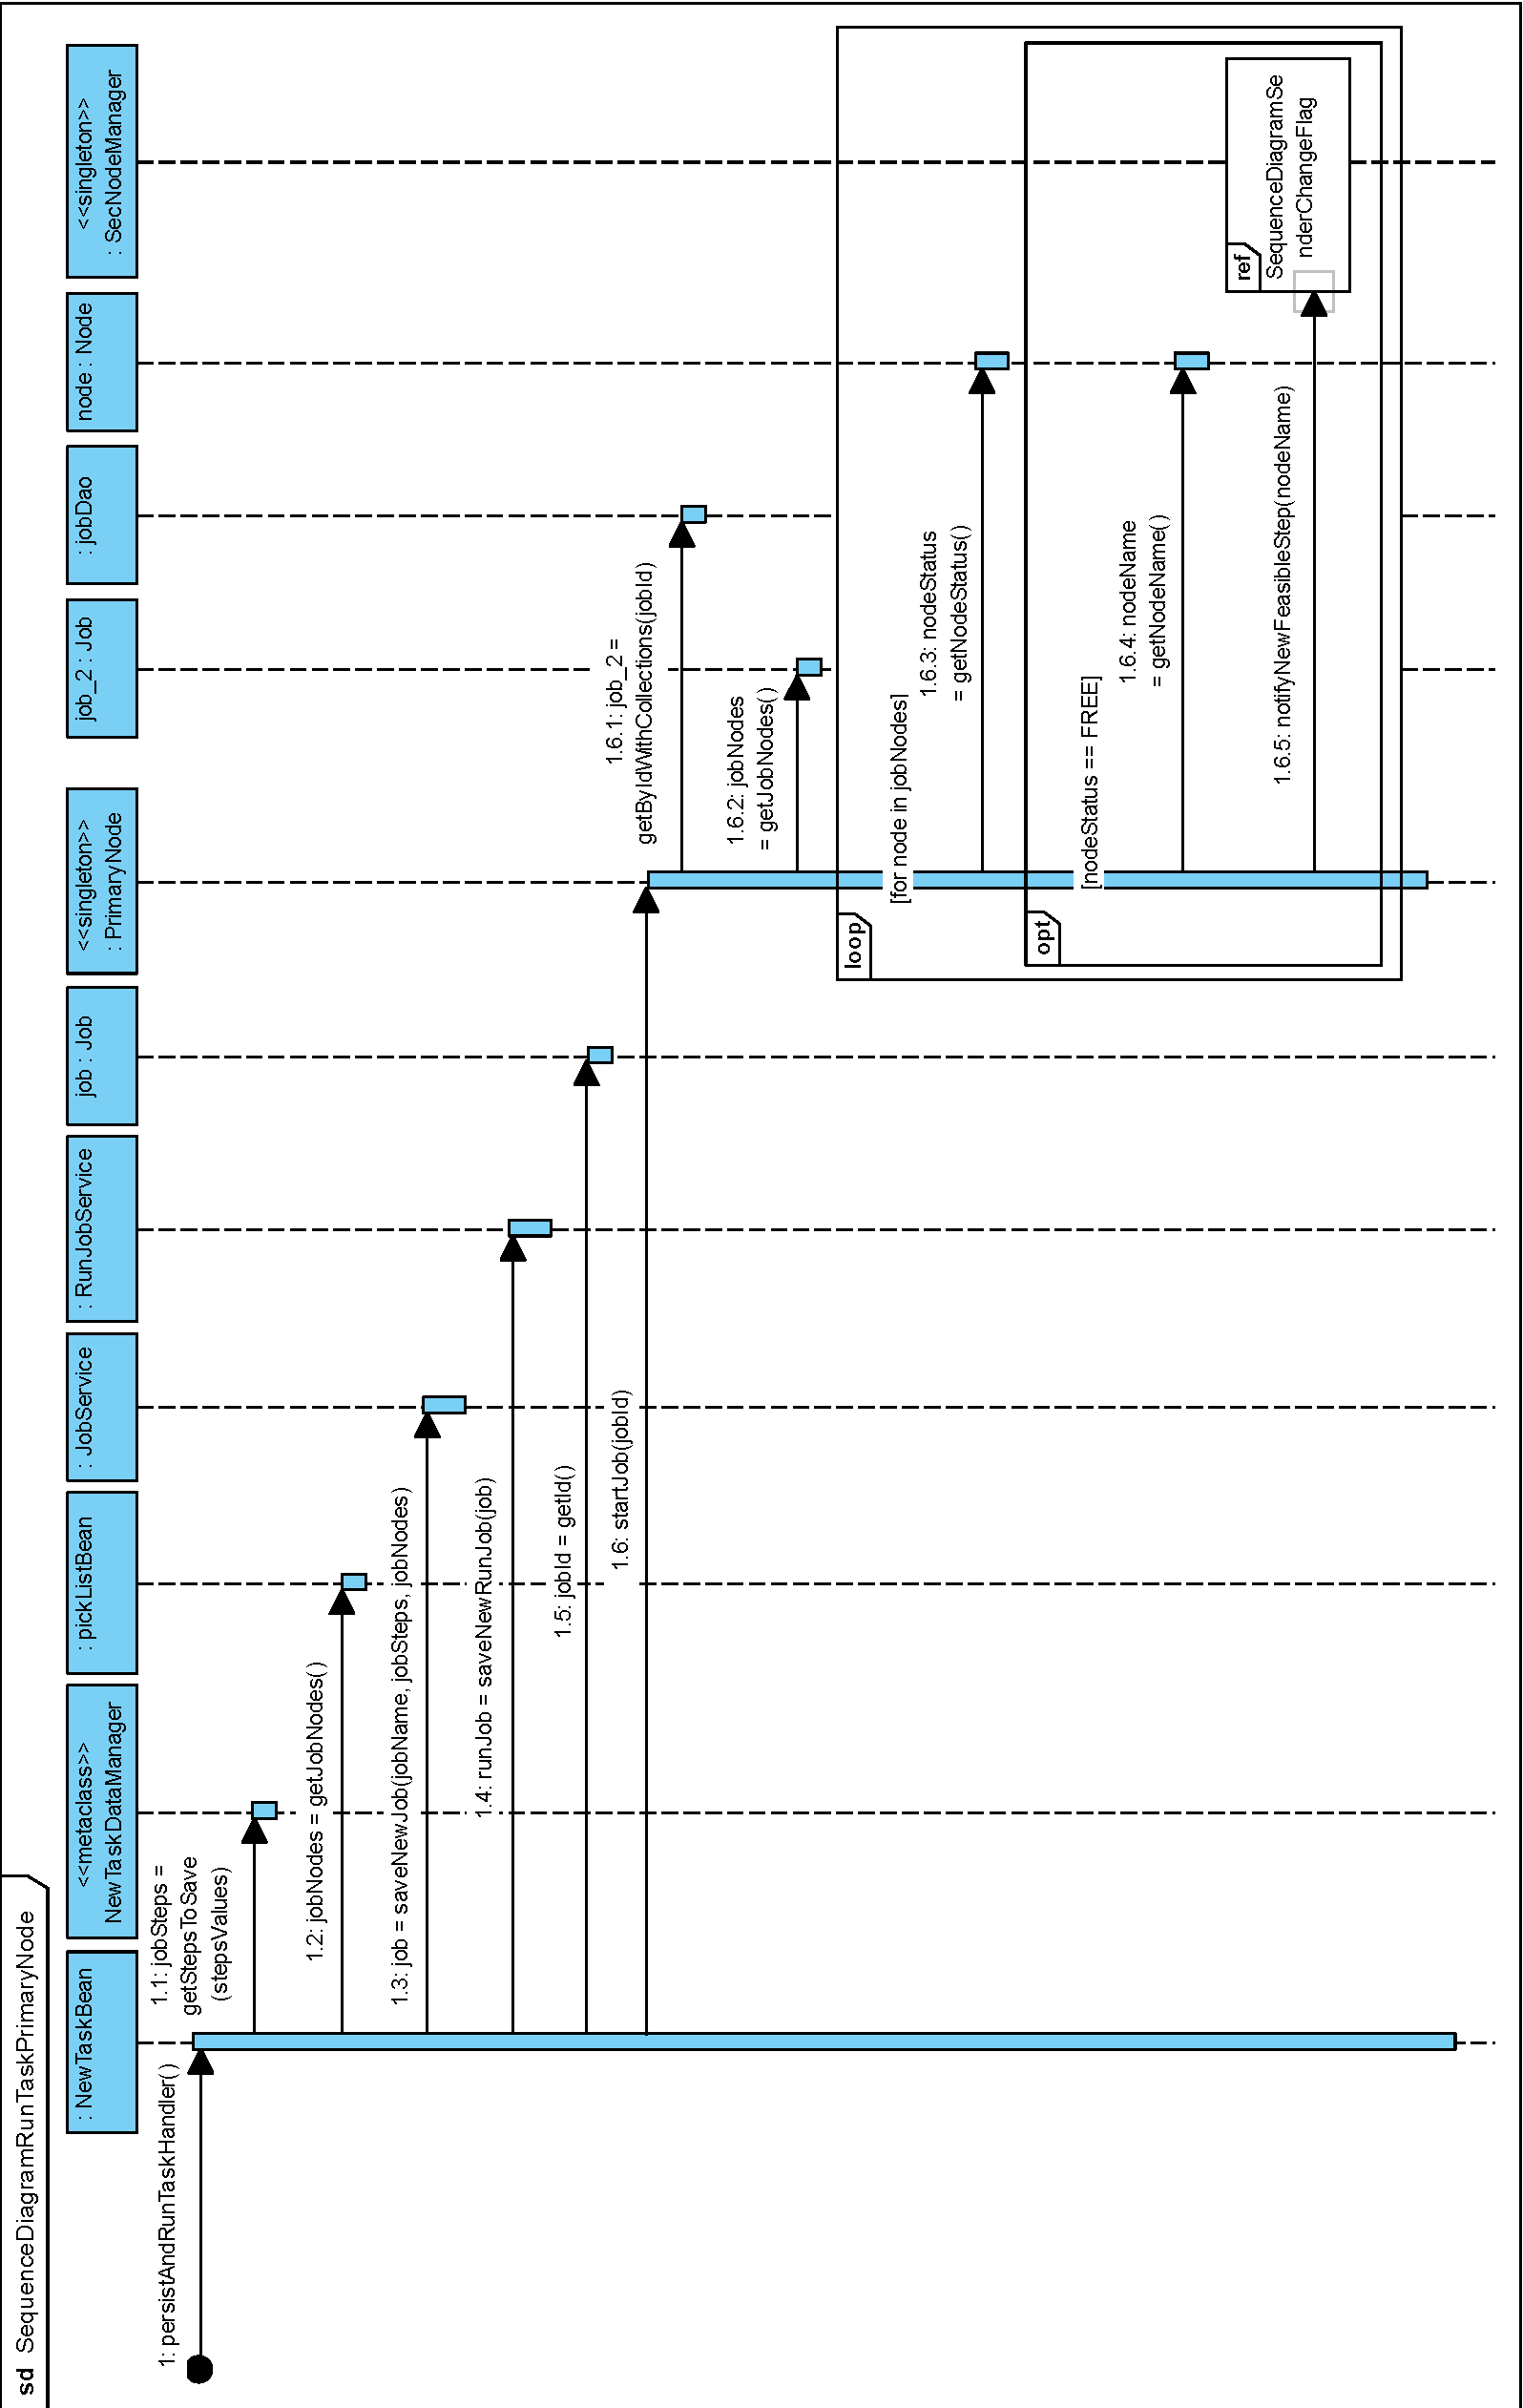
\includegraphics{images/SequenceDiagramRunTaskPrimaryNode.pdf}
    }
    \caption{\label{obr:sequenceDiagramRunTaskPrimaryNode} {\it Sekvenční diagram znázorňující vytvoření a spuštění nové úlohy na centrálním uzlu.}}
\end{center}
\end{figure}

\subsection*{Spuštění kroku úlohy na výpočetním uzlu}
\label{subsection:runStepOfTaskOnSecondaryNode}

Zpracování kroku úlohy na výpočetním uzlu začne přijetím zprávy \textit{RunStepMsg}, jak je možné vidět na obrázku \ref{obr:sequenceDiagramRunTaskSecondaryNode}. Z této zprávy budou následně získány informace potřebné pro jeho spuštění. Tyto informace budou předány třídě \textit{StepExecutor}. Před samotným spuštěním bude nezbytné načíst všechny vstupy, přesněji cesty k těmto vstupům, což bude zajišťovat třída \textit{InputLoader}. Způsob načítání vstupních souborů je možně vidět na obrázku \ref{obr:sequenceDiagramLoadInputsSecondaryNode}. 

Z diagramu je zřejmé, že způsob načítání vstupů bude závislý na typu spuštění. V případě, že mají být zpracovány všechny nezpracované vstupy a typem vstupu bude soubor nebo složka, bude objektu třídy \textit{SecStatusMaintainer}, který bude udržovat stav výpočetního uzlu, předána přijatá vstupní cesta. Pokud bude typem vstupu složka souborů nebo složka složek, budou tomuto objektu předány cesty ke všem souborům, resp. podsložkám, obsaženým ve vstupní složce. Před předáním každého vstupu bude nejprve ověřeno, zda je výstupní soubor nebo složka odpovídající danému vstupu prázdná. Jestliže není, bude tento vstup ze zpracování vynechán. Pokud bude typ spuštění zahrnovat opětovně zpracování vstupů, jejichž zpracování skončilo dříve s chybou, budou tyto chybné vstupy obsažené ve zprávě \textit{RunStepMsg} následně rovněž předány ke zpracování objektu \textit{secStatusMaintainer}. Vzhledem k tomu, že bude pro ukládání vstupů využit zásobník, budou chybné vstupy zpracovány jako první. Jednotlivé typy spuštění jsou popsány v kapitole \ref{section:communicationDesign}. Následně budou v~závislosti na typu výstupu vytvořeny odpovídající výstupní složky. 

Poté budou spuštěna vlákna třídy \textit{StepExecutor}, jejichž počet bude odpovídat počtu procesů, ve kterých má být zpracování daného kroku úlohy prováděno. Postup spuštění v~jednotlivých vláknech je vzhledem ke složitosti uveden v samostatném diagramu na obrázku \ref{obr:sequenceDiagramRunTaskStepStartSecondaryNode}. Z diagramu je zřejmé, že bude z přijatých dat nejprve zjištěn zadaný regulární výraz a parametrizovaná cesta k výstupu. Z objektu udržujícího stav výpočetního uzlu bude načtena cesta k v pořadí dalšímu nezpracovanému vstupu. Z těchto informací bude následně získána skutečná výstupní cesta odpovídající cestě k aktuálnímu vstupu. Postup aplikace regulárního výrazu je detailně popsán v kapitole \ref{subsection:newTaskForm}. Poté bude provedeno samotné spuštění procesu v metodě \textit{startExecutingStep}. Objekt, reprezentující spuštěný proces, bude předán Singleton objektu \textit{UsageValuesSender}. Ten bude s využitím programu \textit{Top}, který je popsán v kapitole \ref{chapter:used_technologies}, získávat informace o aktuálním vytížení výpočetního uzlu všemi spuštěnými procesy zpracovávajícími daný krok a zasílat tyto informace na centrální uzel. Následně bude spuštěno vlákno, které bude v pravidelných intervalech kontrolovat, zda spuštěný proces běží, zda nebyla překročena maximální doba zpracování jednoho vstupu nebo zda nebyl přijat požadavek na zastavení zpracování daného kroku úlohy. Pokud ano, bude proces provádějící krok úlohy ukončen. Pokud daný proces již neběží, budou provedeny výstupní validace, které jsou detailně popsány v kapitole \ref{section:validationDesign}.

Nakonec bude na výpočetní uzel odeslána potvrzující zpráva \textit{RunStepAckMsg} s počtem načtených vstupních souborů. V případě, že nastane v jakékoliv fázi, tj. při načítání vstupů, při běhu procesu vykonávajícího daný krok nebo při výstupních validacích, chyba, bude na centrální uzel odeslána zpráva typu \textit{ProcErrorMsg} obsahující detaily o chybě, která nastala.

\begin{figure}[H]
\begin{center}
    \scalebox{0.5}
    {
        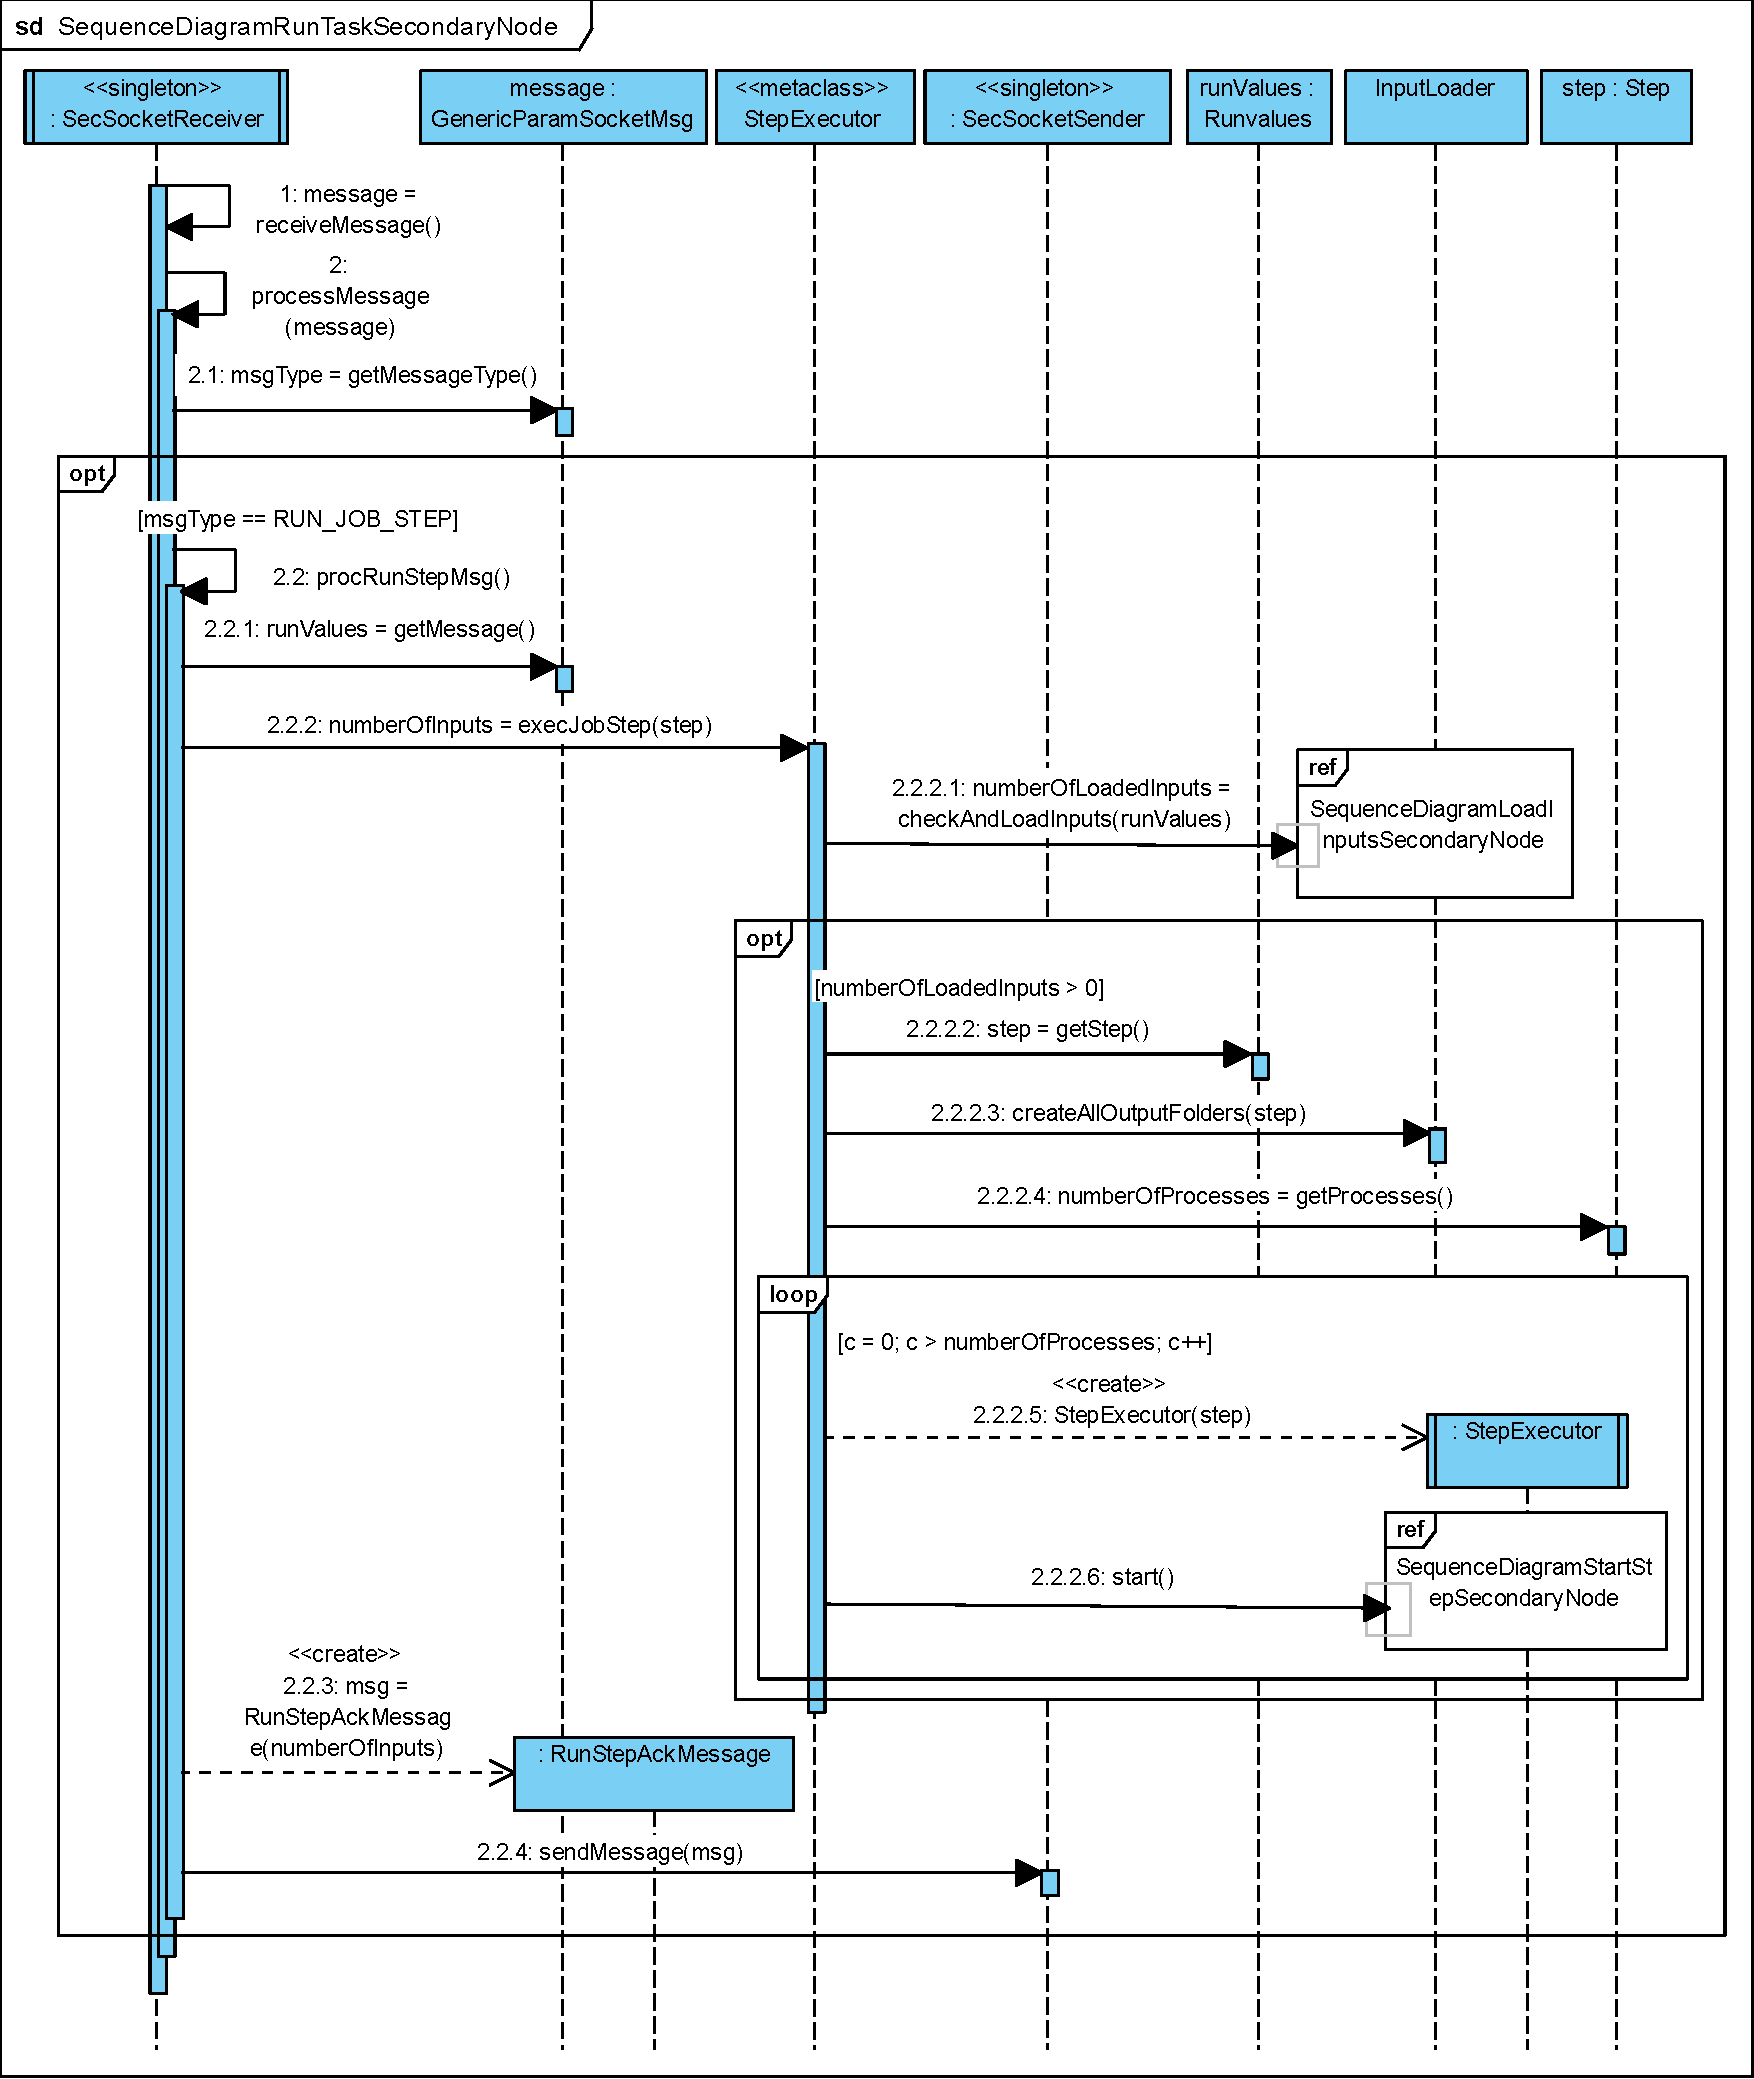
\includegraphics{images/SequenceDiagramRunTaskSecondaryNode.pdf}
    }
    \caption{\label{obr:sequenceDiagramRunTaskSecondaryNode} {\it Sekvenční diagram znázorňující přijetí požadavku na zpracování kroku úlohy na výpočetním uzlu.}}
\end{center}
\end{figure}

\begin{figure}[H]
\begin{center}
    \scalebox{0.5}
    {
        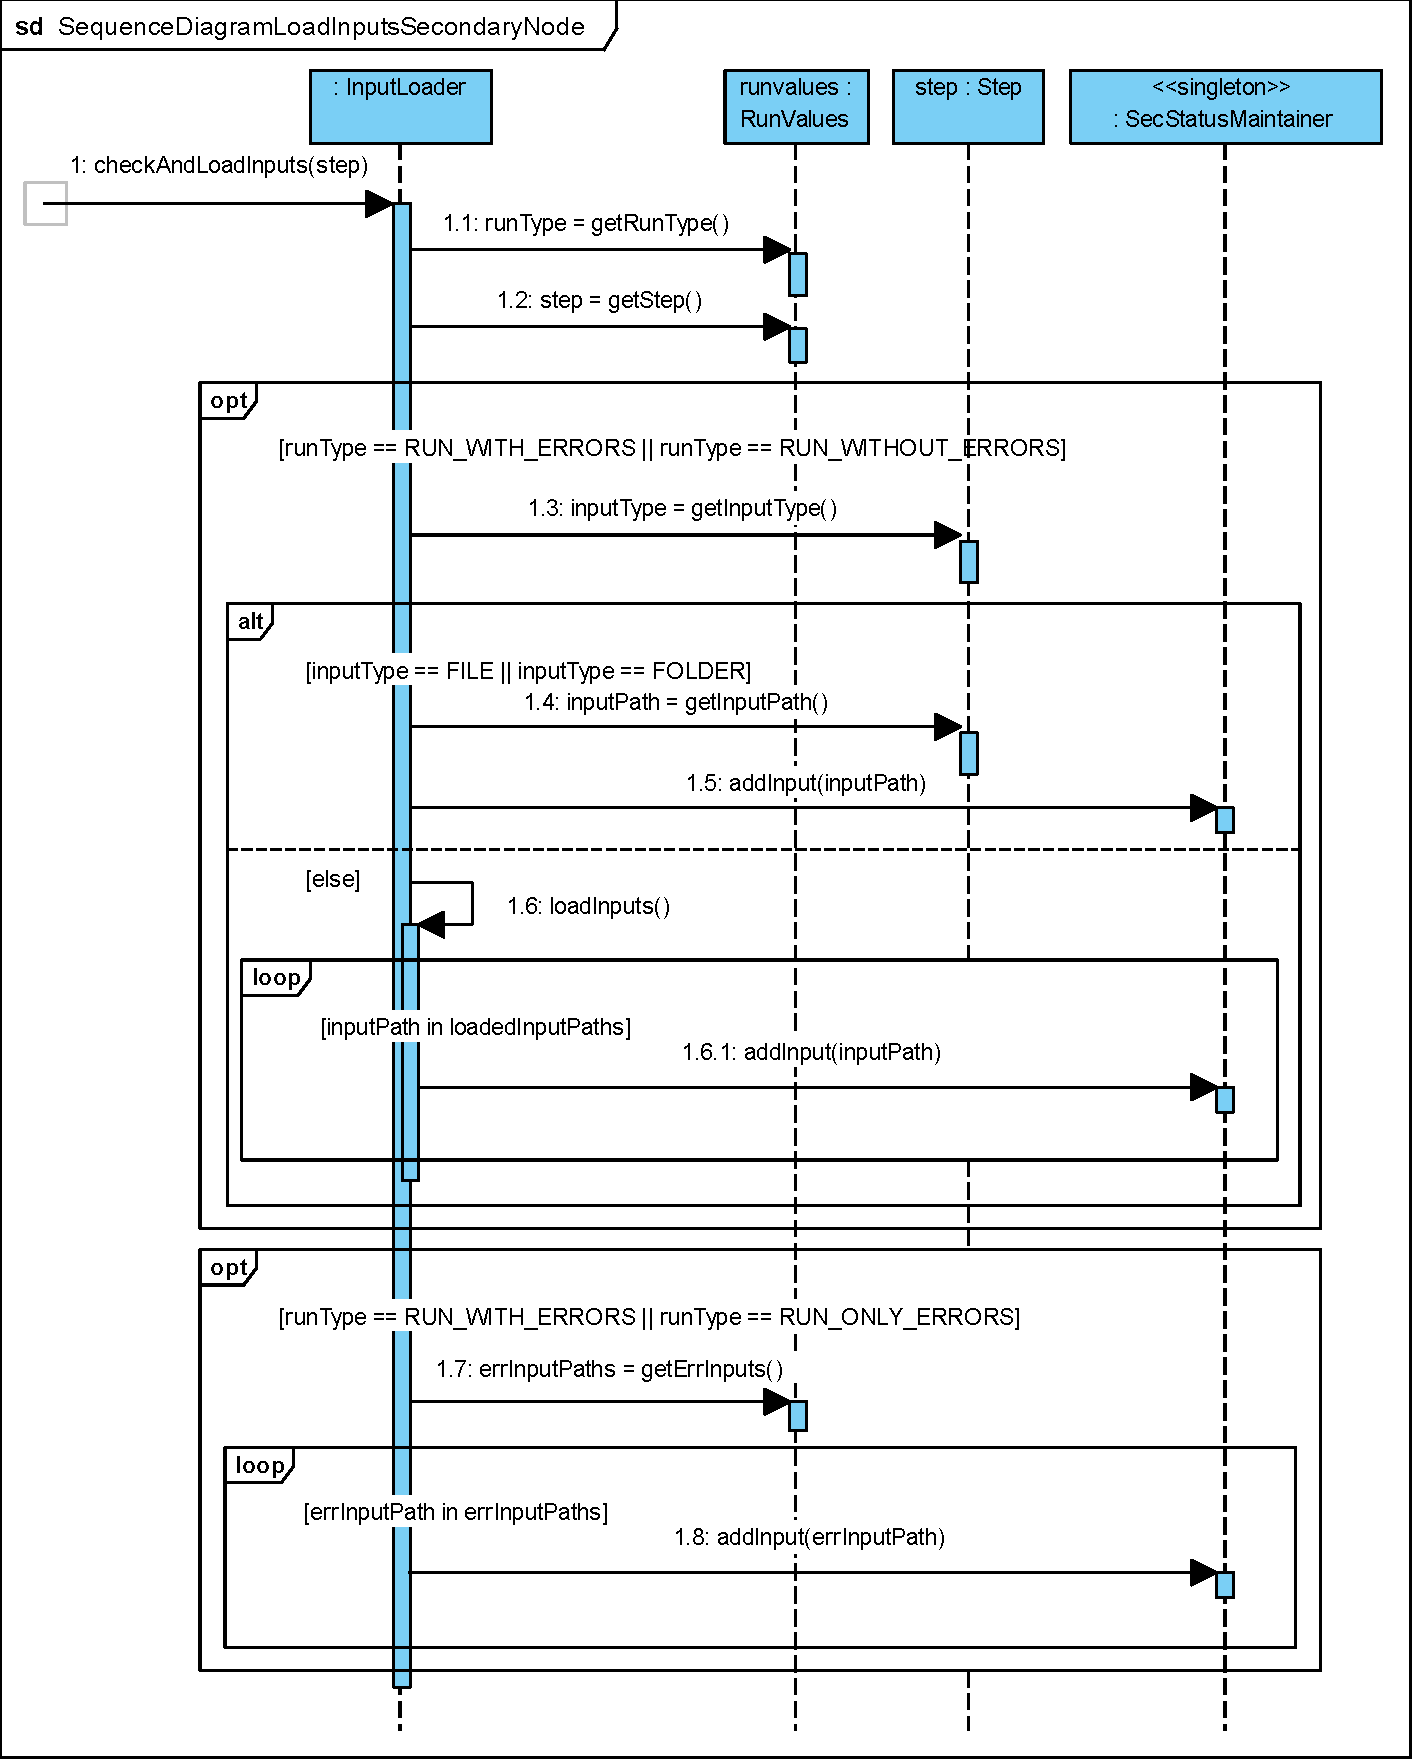
\includegraphics{images/SequenceDiagramLoadInputsSecondaryNode.pdf}
    }
    \caption{\label{obr:sequenceDiagramLoadInputsSecondaryNode} {\it Sekvenční diagram znázorňující načtení vstupů ke zpracování na výpočetním uzlu.}}
\end{center}
\end{figure}

\begin{figure}[H]
\begin{center}
    \scalebox{0.5}
    {
        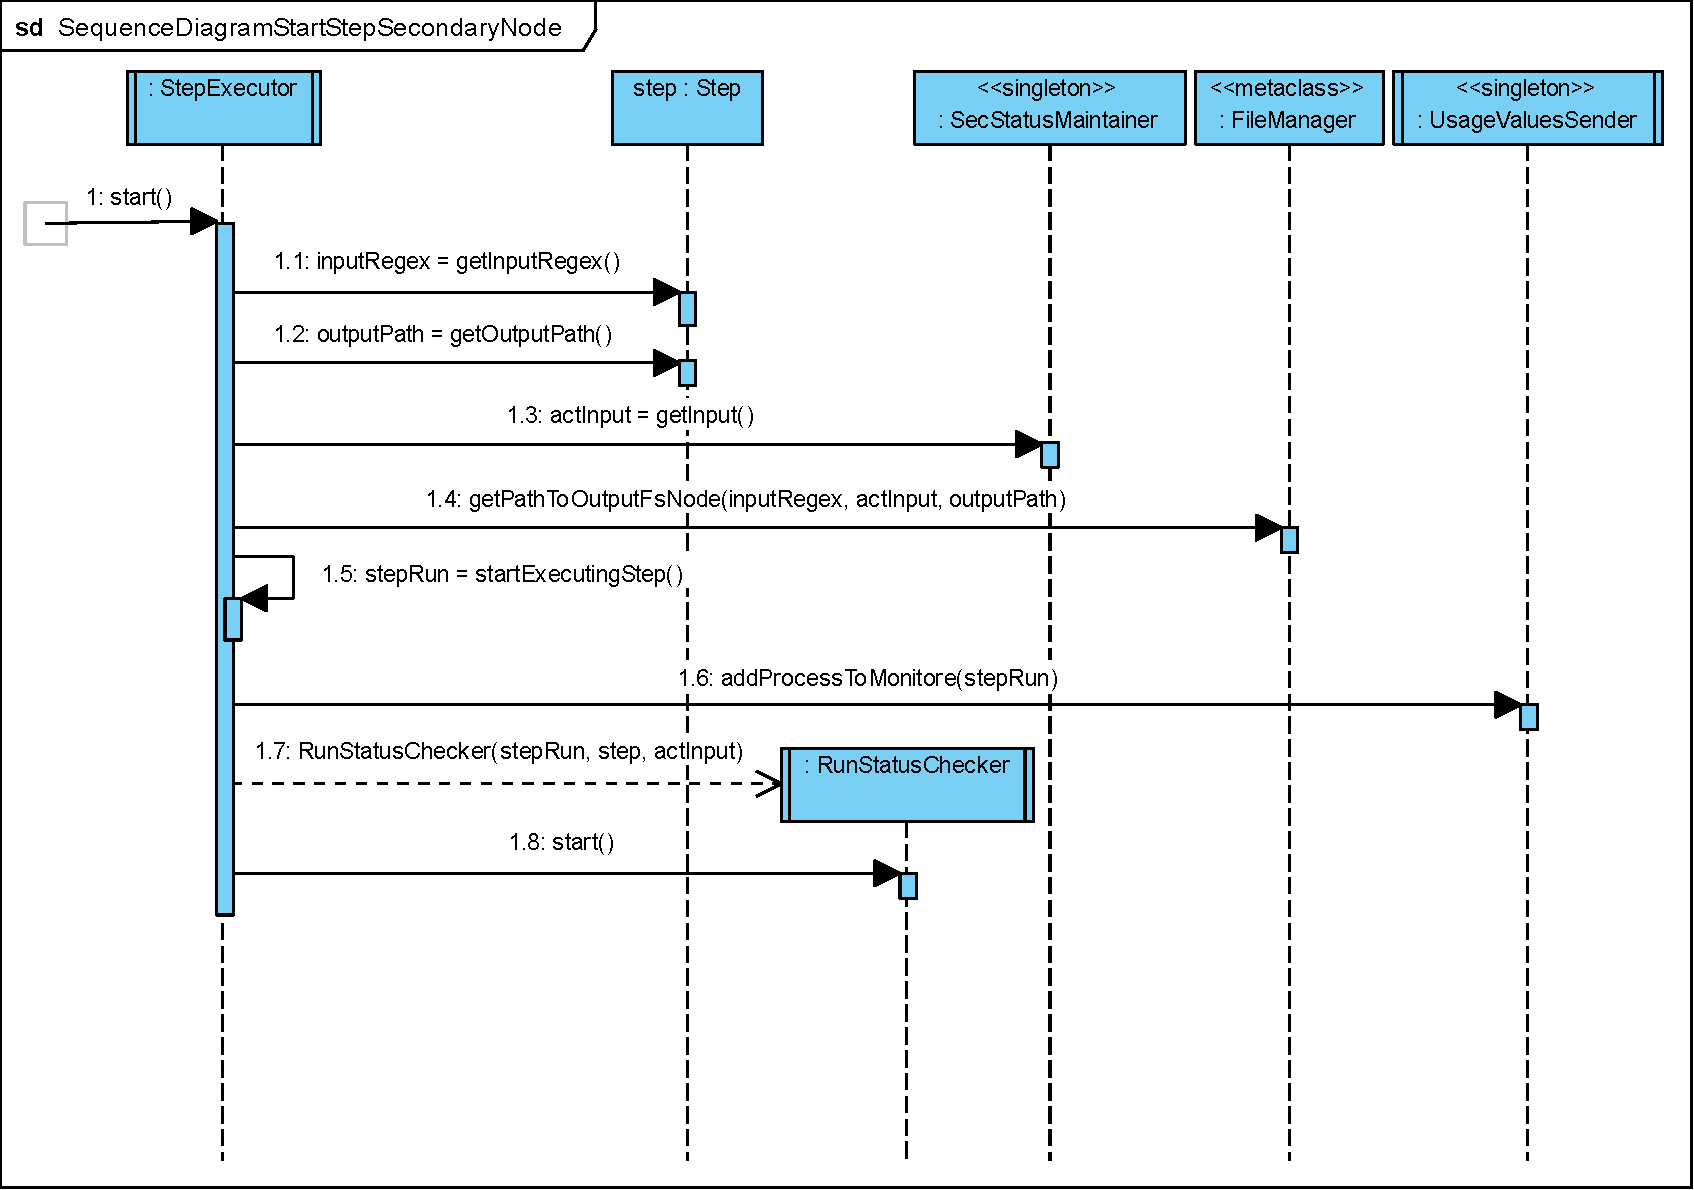
\includegraphics{images/SequenceDiagramStartStepSecondaryNode.pdf}
    }
    \caption{\label{obr:sequenceDiagramRunTaskStepStartSecondaryNode} {\it Sekvenční diagram znázorňující spuštění zpracování kroku úlohy na výpočetním uzlu.}}
\end{center}
\end{figure}

\section{Spuštění opětovného zpracování chybných vstupů}
\label{section:RerunTaskOnPrimaryNode}

Spuštění opětovného zpracování chybných vstupů začíná na centrálním uzlu zavoláním metody odpovídajícího backing beanu pro obsluhu požadavku od klienta, jak je znázorněno v diagramu na obrázku \ref{obr:sequenceDiagramRerunErrorInputsPrimaryNode}. Na diagramu je dále možné vidět, že v této metodě bude stejně jako v případě spuštění nové úlohy předán požadavek na EJB bean \textit{PrimaryNode}. Zde budou načtena data o rozpracovaném kroku úlohy na zadaném výpočetním uzlu. 

\begin{figure}[H]
\begin{center}
    \scalebox{0.5}
    {
        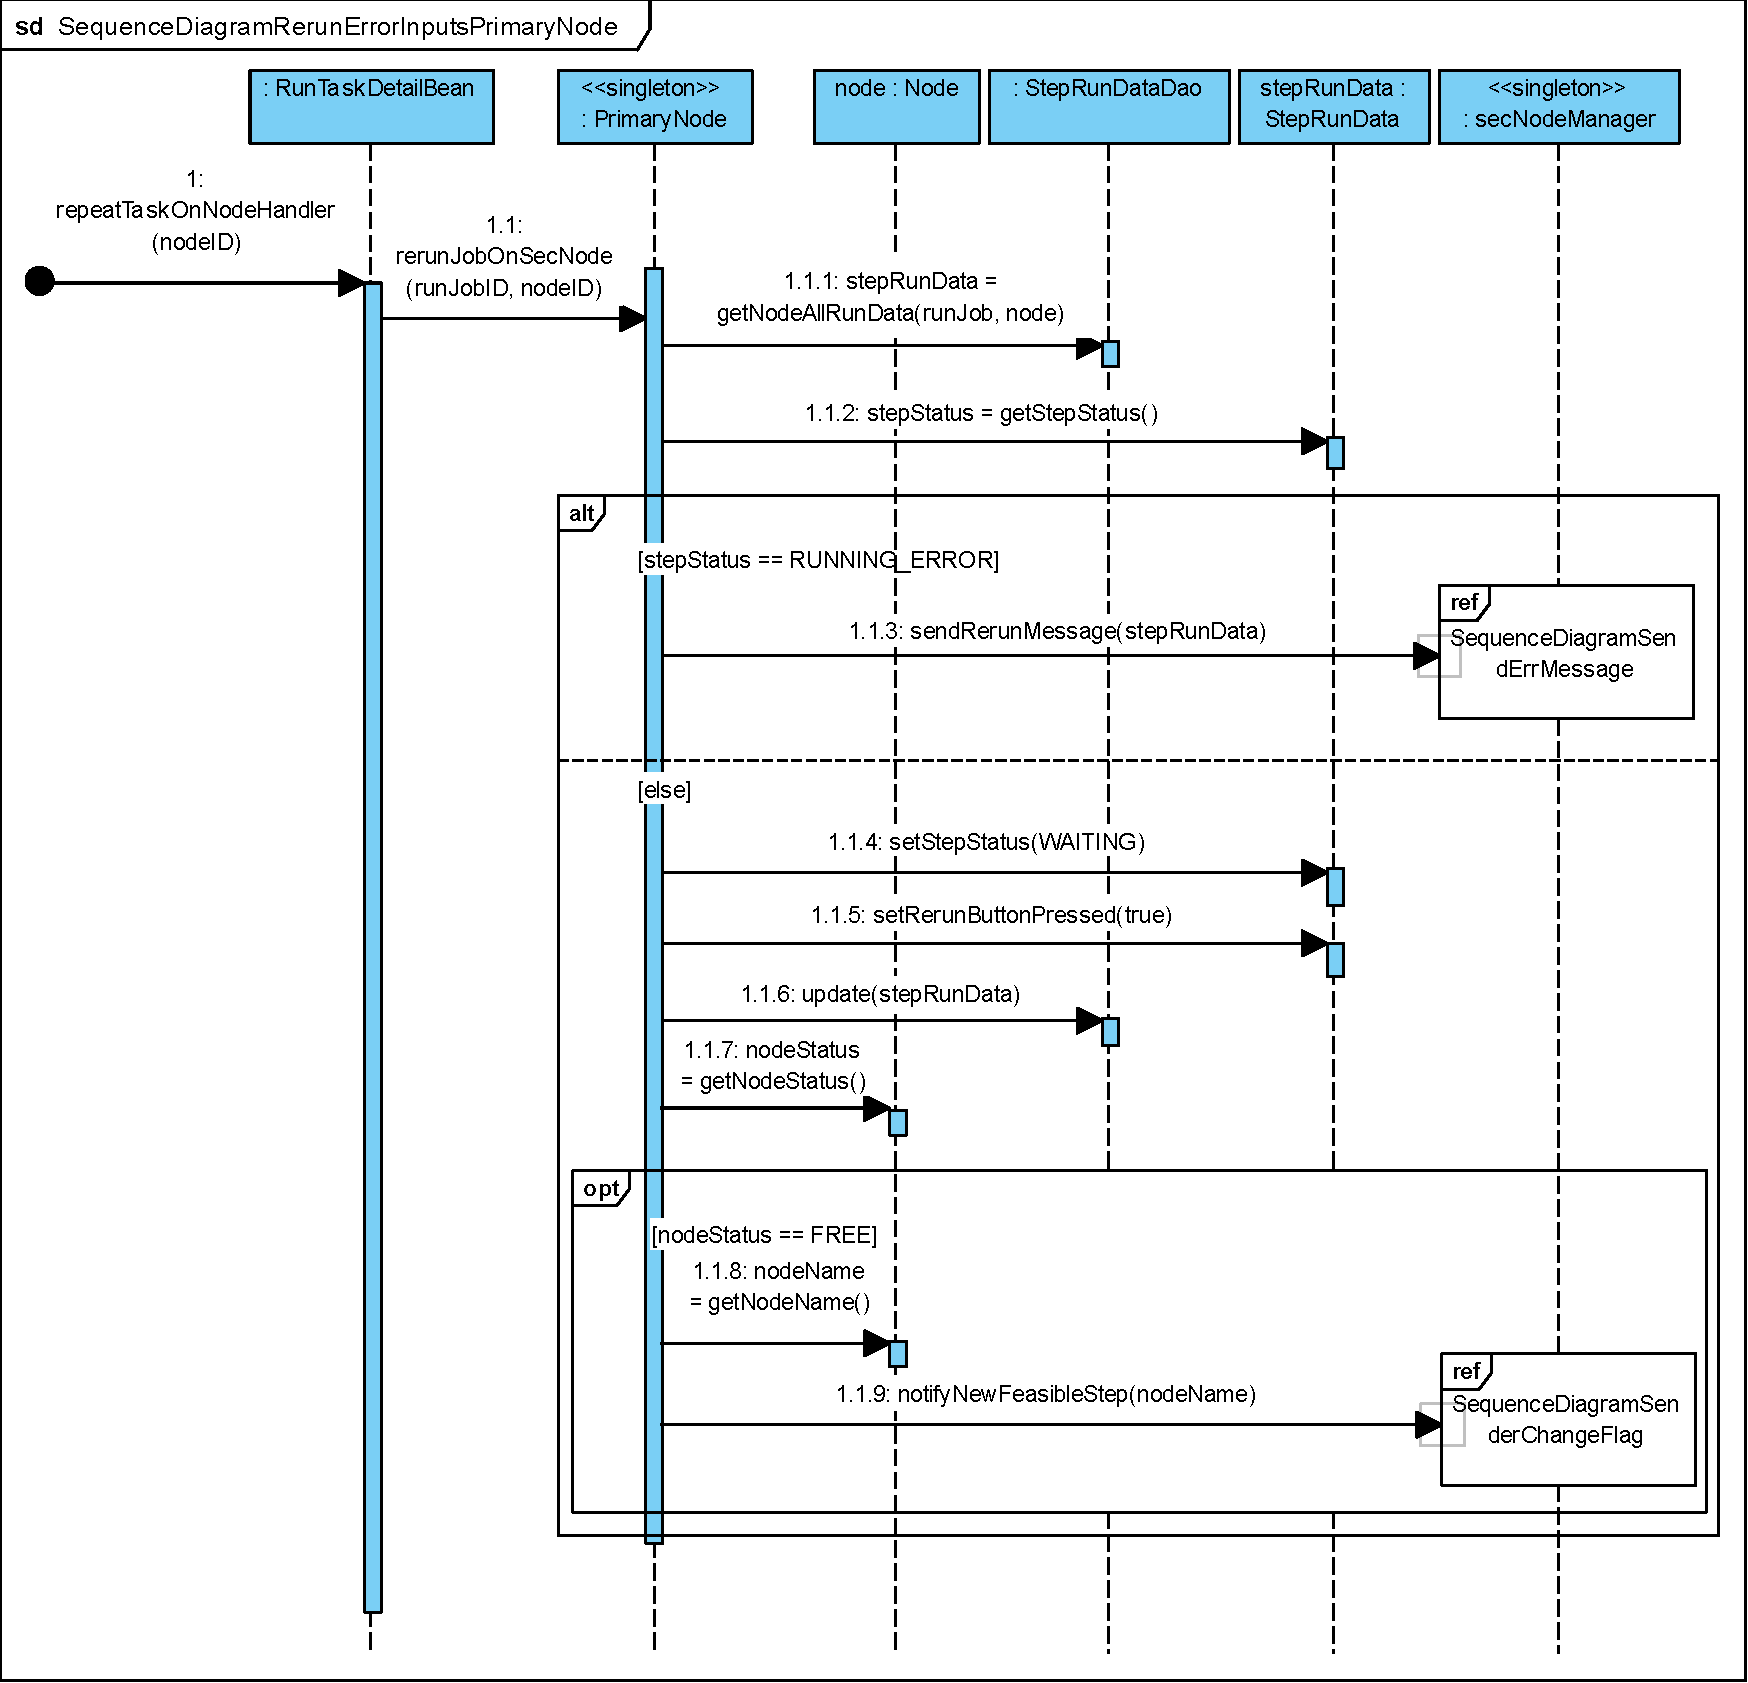
\includegraphics{images/SequenceDiagramRerunErrorInputsPrimaryNode.pdf}
    }
    \caption{\label{obr:sequenceDiagramRerunErrorInputsPrimaryNode} {\it Sekvenční diagram znázorňující spuštění opětovného zpracování chybných vstupů na centrálním uzlu.}}
\end{center}
\end{figure}


Pokud tento krok na daném výpočetním uzlu stále běží, tedy nachází se ve stavu \textit{RUNNING\_ERROR}, bude na něj odeslána zpráva \textit{RerunMsg} obsahující seznam chybných vstupů. Pro přehlednost je odeslání této zprávy a~přijetí potvrzující zprávy znázorněno v~samostatném diagramu na obrázku \ref{obr:sequenceDiagramSendErrMessagePrimaryNode}. Na diagramu je vidět, že odeslání probíhá získáním objektu \textit{SecNodeCommunicator} pro konkrétní výpočetní uzel, ze kterého je následně získán objekt pro odesílání zpráv pomocí něhož je zpráva odeslána.

\begin{figure}[H]
\begin{center}
    \scalebox{0.49}
    {
        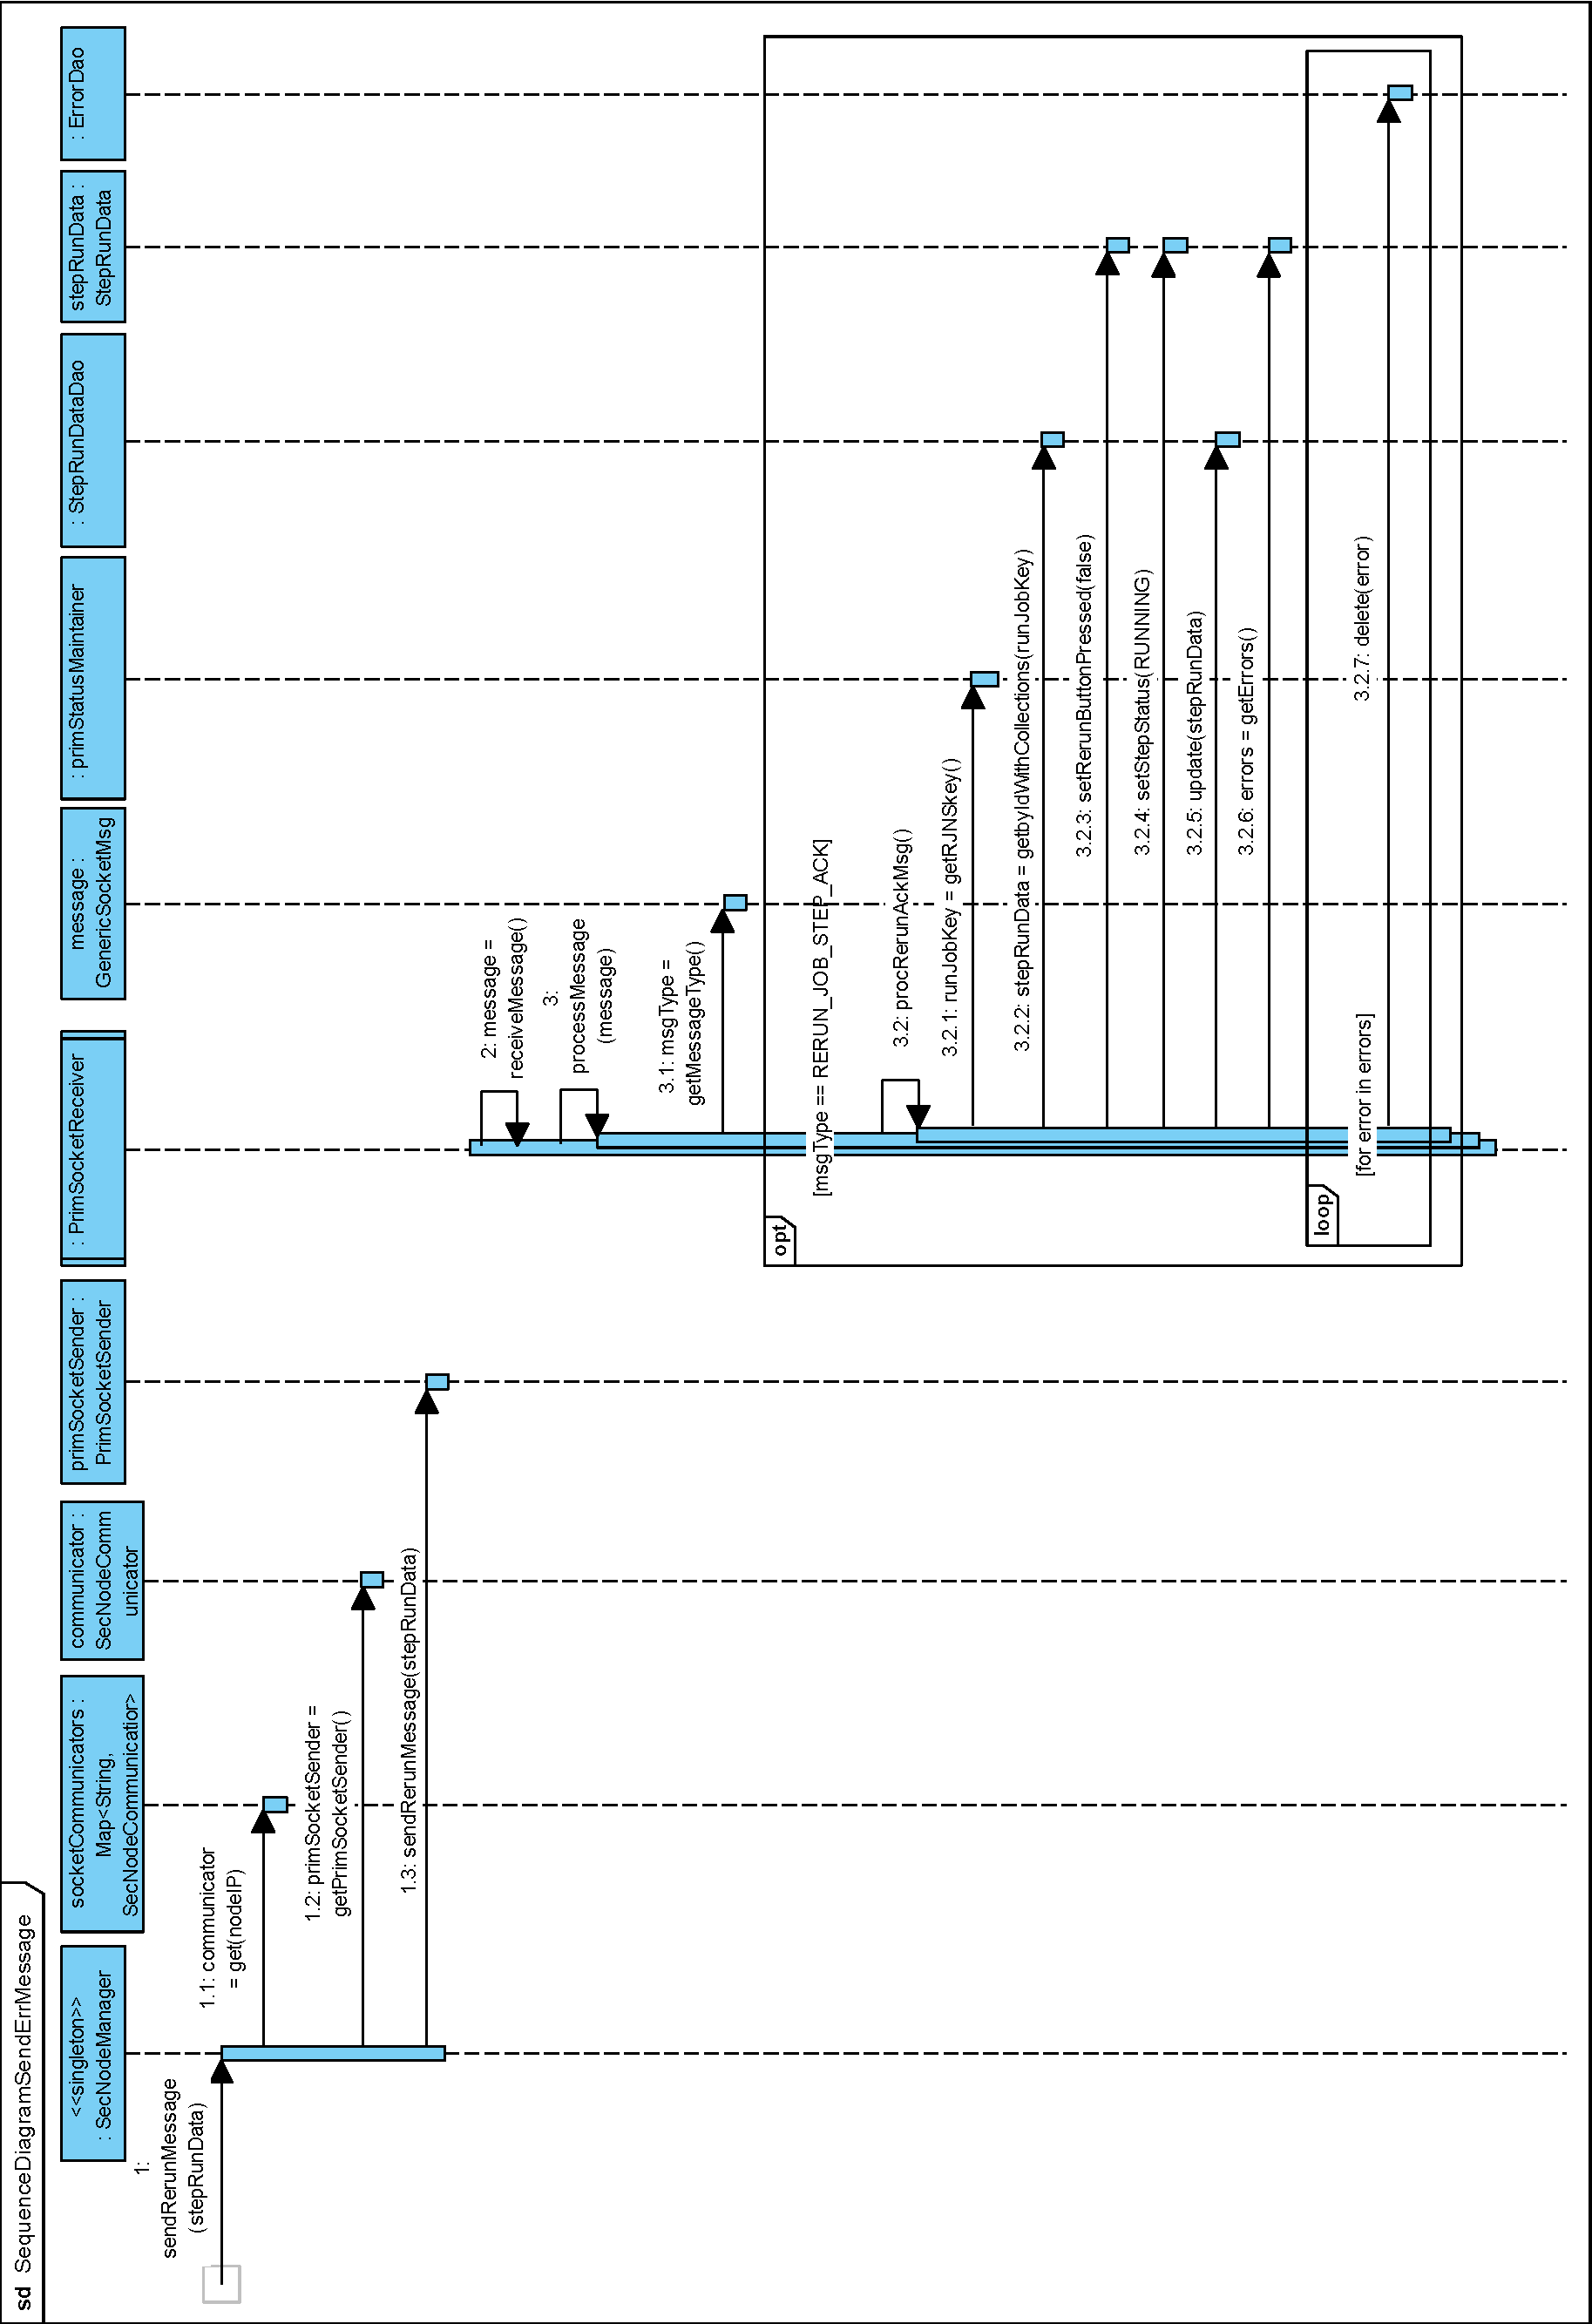
\includegraphics{images/SequenceDiagramSendErrMessagePrimaryNode.pdf}
    }
    \caption{\label{obr:sequenceDiagramSendErrMessagePrimaryNode} {\it Sekvenční diagram  znázorňující odeslání zprávy pro opětovné spuštění chybných vstupů na výpočetní uzel a zpracování potvrzující zprávy.}}
\end{center}
\end{figure}

Po přijetí této zprávy na výpočetním uzlu budou z této zprávy získány chybné vstupy. Ty budou předány objektu \textit{secStatusMaintainer}, který udržuje aktuální stav výpočetního uzlu, kde budou přidány do zásobníku nezpracovaných vstupů. Nakonec bude na centrální uzel odeslána potvrzující zpráva \textit{RerunAckMsg}. Zpracování zprávy \textit{RerunMsg} na výpočetním uzlu je možné vidět na obrázku \ref{obr:sequenceDiagramProcessRerunMessageSecondaryNode}.

\begin{figure}[H]
\begin{center}
    \scalebox{0.5}
    {
        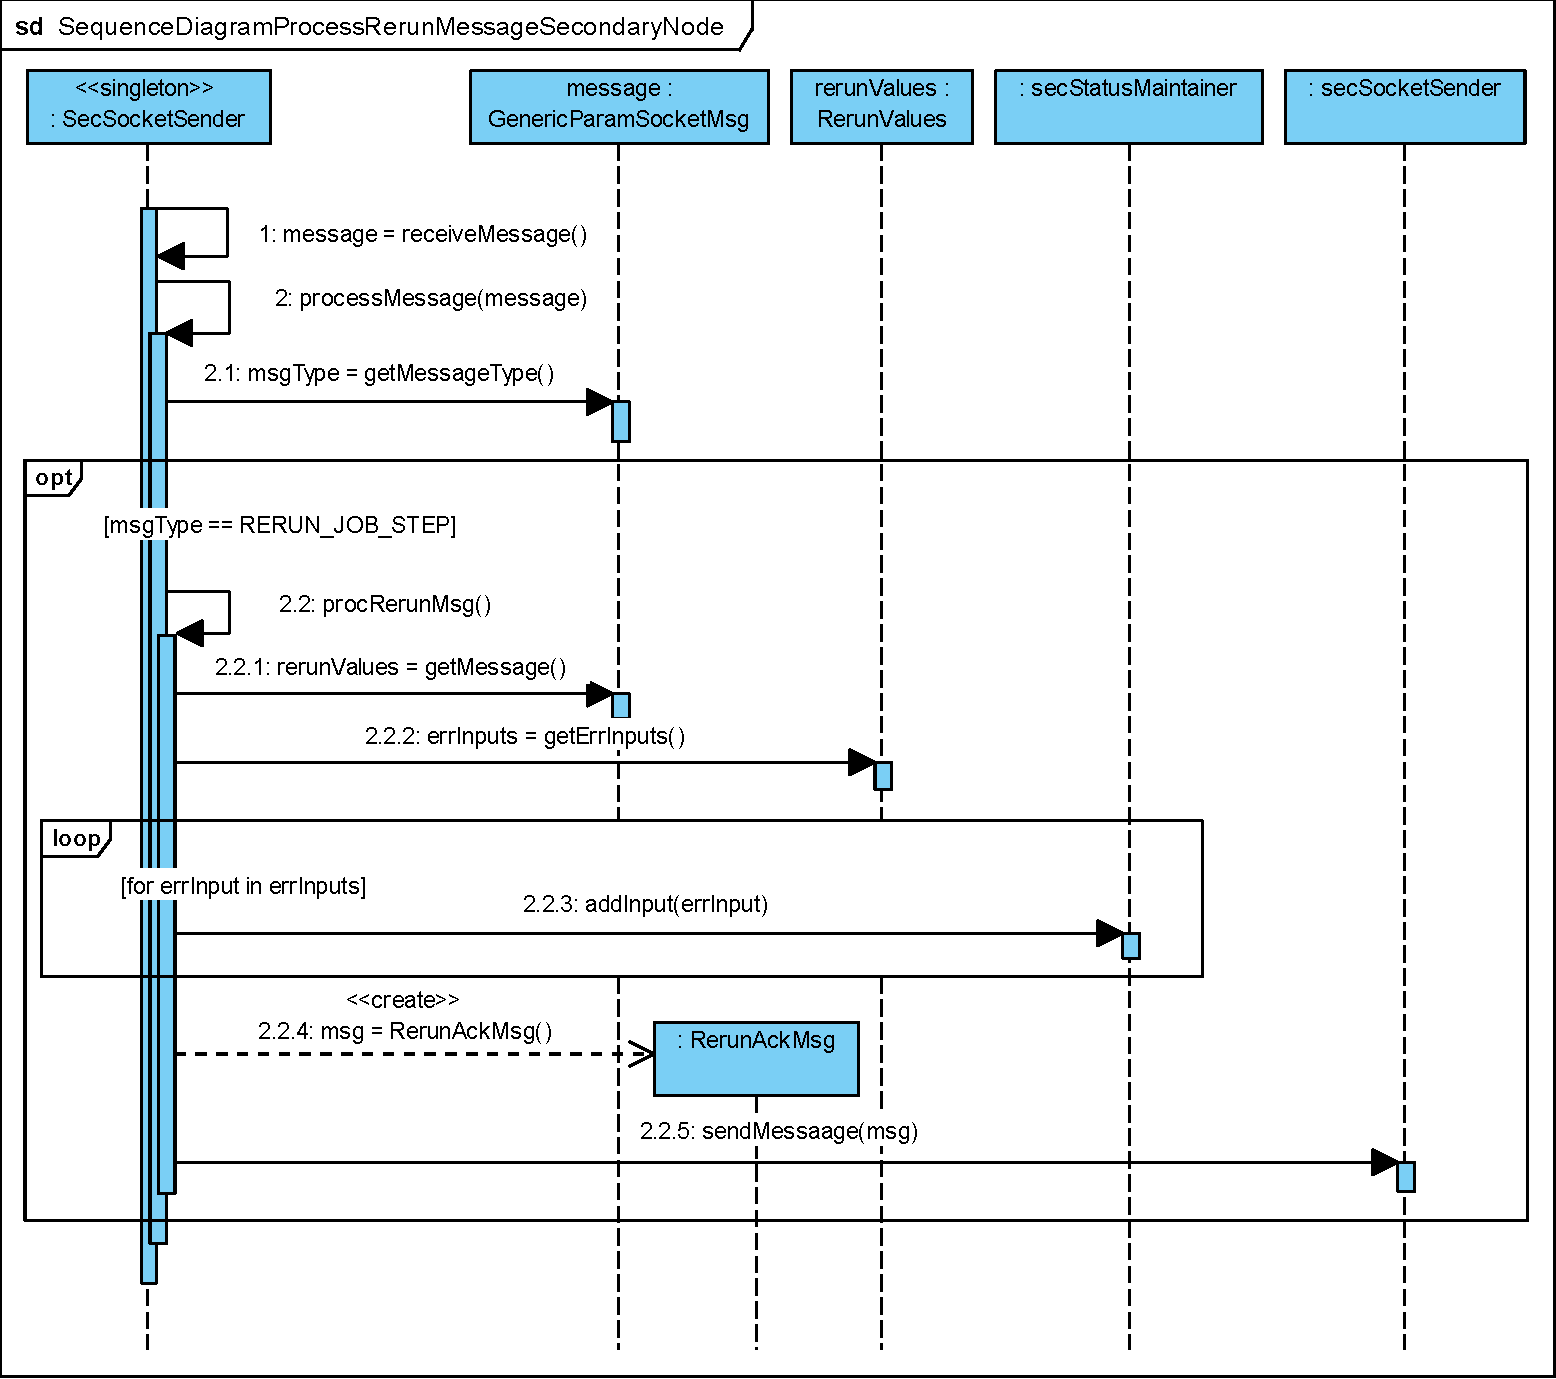
\includegraphics{images/SequenceDiagramProcessRerunMessageSecondaryNode.pdf}
    }
    \caption{\label{obr:sequenceDiagramProcessRerunMessageSecondaryNode} {\it Sekvenční diagram znázorňující přijetí požadavku na opětovné zpracování chybných vstupů na výpočetním uzlu.}}
\end{center}
\end{figure}

Z diagramu na obrázku \ref{obr:sequenceDiagramSendErrMessagePrimaryNode} je dále možné vidět, že po přijetí potvrzující zprávy \textit{RerunAckMsg} je změněn stav kroku a informace o chybných vstupech jsou z databáze vymazány.


Pokud tento krok na daném výpočetním uzlu již neběží, tj. je ve stavu \textit{ERROR}, aktualizuje se jeho stav na \textit{WAITING}, čímž se zařadí do implicitní fronty proveditelných kroků. Dále bude nastaven příznak, který označuje, že se jedná o požadavek na opětovné zpracování chybných vstupů. Tento krok je nezbytný k tomu, aby bylo při odesílání daného kroku úlohy na výpočetní uzel možné rozlišit tento požadavek od požadavku na spuštění pozastavené úlohy, případně zda se nejedná o obě možnosti současně. Když je daný uzel volný, je navíc provedena změna příznaku u odesílatele zpráv na daný výpočetní uzel pro opětovnou kontrolu proveditelného kroku stejným způsobem, jako v případě vytvoření nové úlohy, což je detailně popsáno v kapitole \ref{subsection:runStepOfTaskOnSecondaryNode}. Diagram znázorňující zajištění opětovné kontroly proveditelného kroku je možné vidět na obrázku \ref{obr:sequenceDiagramRunTaskPrimaryNodeSenderChangeFlag}.

%\section{Diagram nasazení (zatím není jisté)} \todo{Udělat jej ??}

%%%%%%%%%%%%%%%%%%%%%%%%%%%%%%%%%%%%%%%%%%%%%%%%%%%%%%%%%%%%%%%%%%%%%%%%%%%%%%%%%%%%%%%%%%%%%%%%%%%%%%%%%%%%%%%%%%

\chapter{Implementace}
\label{chapter:implementation}

V této kapitole jsou popsány implementační detaily vybraných částí celého systému. Pozornost je věnována nejzajímavějším částem obou aplikací a odlišnostem reálné aplikace od jejího návrhu.

\section{Monitorování běhu úlohy na výpočetním uzlu}

Při spuštění úlohy na výpočetním uzlu jsou nejprve načteny cesty ke všem vstupům a~následně jsou vytvořena vlákna třídy \textit{StepExecutor}, která zajišťují spouštění samotných procesů zpracovávajících jednotlivé vstupy daného kroku úlohy, přičemž platí, že počet vytvořených vláken odpovídá počtu paralelně běžících procesů, které mají daný krok úlohy zpracovávat. Toto vlákno dále vytvoří vlákno třídy \textit{RunStatusChecker}, jehož úkolem je monitorovat spuštěný proces. Referenci na spuštěný proces dále předá vláknu \textit{UsageValuesSender}, které monitoruje využití systémových prostředků daným procesem, jak je uvedeno v kapitole \ref{section:RunTask}. Jakmile je zpracování daného vstupu dokončeno, je spuštěn nový proces zpracování s~v~pořadí dalším nezpracovaným vstupem a~celý postup se opakuje. Jakmile nejsou k dispozici další vstupy pro zpracování, je vlákno ukončeno.

Reference na každý spuštěný proces provádějící daný krok úlohy je předána objektu třídy \textit{UsageValuesSender} implementujícímu návrhový vzor Singleton, který obsahuje seznam všech aktuálně spuštěných procesů. Monitorování využití systémových prostředků je realizováno pomocí programu \textit{Top}. Ten je spouštěn každých 5~vteřin, přičemž hodnoty využití systémových prostředků jsou odečítány každou vteřinu. Ve výchozím nastavení je pro využití paměti RAM zobrazována hodnota RES, která odpovídá velikosti skutečně obsazené paměti RAM daným procesem. Vzhledem k tomu, že při spuštění úlohy může daný proces zabírat i~část paměti SWAP, je nutné odečítat hodnotu USED, která odpovídá součtu hodnot obsazené paměti RAM a~obsazené paměti SWAP. Aby bylo možné hodnotu USED vyčítat, je nutné změnit výchozí formát výstupu programu \textit{Top}. Tento formát není možné specifikovat pomocí parametru příkazové řádky, ale lze jej změnit pouze interaktivně při spuštění programu. Konfigurace je poté pro daného uživatele uložena do souboru \textit{\$HOME/.toprc} odkud je následně při každém dalším spuštění automaticky načítána. Cestu k~tomuto konfiguračnímu souboru rovněž nelze změnit pomocí parametru. Aby nebylo nutné měnit formát výstupu ručně na každém výpočetním uzlu zvlášť, je před každým spuštěním tohoto programu nastavena proměnná prostředí \textit{\$HOME} tak, aby obsahovala cestu k již vytvořenému konfiguračnímu souboru. Vzhledem k tomu, že jsou všechny výpočetní uzly připojeny ke společnému síťovému disku, stačí mít jeden konfigurační soubor společný pro všechny výpočetní uzly.

Z takto upraveného výstupu jsou následně získány hodnoty obsazenosti paměti RAM a~vytíženosti CPU týkající se pouze procesů provádějících daný krok úlohy. Vzhledem k~tomu, že mohou být hodnoty obsazenosti paměti RAM v různých jednotkách, jsou převedeny na GiB. Vytíženost CPU je vyčítána v procentech, takže ji není nutné převádět. Tato data jsou následně roztříděna dle \texttt{pid} (process identifier) a~pro každý proces zprůměrována. Průměrné hodnoty vytíženosti odpovídající jednotlivým procesům jsou poté sečteny. Jelikož každý proces zpravidla vytěžuje jedno jádro, může být výsledná hodnota vytíženosti CPU vyšší než 100\,\%. Takto získané informace jsou poté odeslány na centrální uzel ve zprávě \textit{UsageMsg}. Před každým spuštěním programu \textit{Top} je u každého monitorovaného procesu ověřeno, zda stále běží. Pokud byl již daný proces ukončen, je ze seznamu monitorovaných procesů automaticky odstraněn.

Vlákno třídy \textit{RunStatusChecker} je pravidelně spouštěno každých 500~ms. V tomto vlákně je periodicky kontrolováno, zda spuštěný proces stále běží. Pokud již skončil, je načten chybový výstup, ověřen návratový kód a~následně jsou provedeny výstupní validace. V závislosti na tom, zda jsou validace úspěšné, je na centrální uzel zaslána zpráva \textit{ProcFinishedMsg} obsahující informaci o~délce zpracování daného vstupu, nebo zpráva typu \textit{ProcErrorMsg}, která navíc obsahuje popis chyby a v závislosti na nastavení při spuštění úlohy i obsah standardního chybového výstupu, případně obsah zadaného logovacího souboru. Při každém spuštění tohoto vlákna je dále ověřováno, zda nebyl přijat požadavek na zastavení provádění daného kroku. V případě že ano, je běžící proces okamžitě ukončen, stejně jako v případě, kdy byla překročena maximální doba zpracování jednoho vstupu.

\section{Odlišnosti v implementaci oproti návrhu}

%\subsection*{Odlišnosti v implementaci obrazovky zobrazující aktuální stav úlohy na jednotlivých výpočetních uzlech}
Při implementaci detailu aktuálně spuštěné úlohy bylo zjištěno, že by bylo velmi problematické zobrazit v tabulce aktuálně rozpracovaných kroků celkový počet vstupů ke zpracování. V případě, že na některém výpočetním uzlu nebyl doposud daný krok úlohy spuštěn, by totiž nebyla zobrazovaná data relevantní, jelikož je celkový počet vstupů ke zpracování na daném uzlu zjišťován až při prvním spuštění daného kroku. Místo tohoto sloupce je tedy v~tabulce zobrazován počet uzlů, na kterých je zpracování daného kroku úspěšně dokončeno.

U této obrazovky byl rovněž upraven způsob filtrování tabulky zobrazující aktuální stav úlohy na jednotlivých výpočetních uzlech. Při realizaci se ukázalo, že by bylo umístění filtrovacího formuláře vedle samotné tabulky velmi problematické. Primefaces navíc obsahují komponentu přímo podporující filtrování a~řazení tabulek. Z~důvodu přehlednosti zobrazovaných dat tak nebyl tento formulář implementován. Původní návrh obrazovky pro detail běžící úlohy je možné vidět na obrázku \ref{obr:wireframe_taskDetail}. Snímek obrazovky skutečné aplikace je pak pro porovnání možné vidět na obrázku \ref{obr:runTaskDetailRealApp}.

U obrazovky zobrazující detail dokončené úlohy se během implementace ukázalo, že zobrazení grafů vedle sebe tak, jak bylo navrženo na obrázku \ref{obr:wireframe_finishedTaskDetail_2}, není příliš vhodné. V~případě spuštění úlohy na více než 20~výpočetních uzlech byla data zobrazovaná v grafech velmi špatně čitelná. Pro větší přehlednost tak byly tyto grafy umístěny pod sebe a~u~každého grafu byla přidána možnost zvolit si libovolnou kombinaci zobrazení minimální, průměrné a~maximální hodnoty. Navíc byl do statistik přidán graf znázorňující minimální a maximální dobu zpracování jednoho vstupu normalizovanou velikostí daného vstupu. U obou grafů znázorňujících normalizovanou i nenormalizovanou dobu zpracování pak byla navíc doplněna možnost zobrazit si název vstupní složky nebo souboru, jehož zpracování trvalo minimální nebo maximální dobu.
\enlargethispage{\baselineskip}
\begin{figure}[H]
    \begin{center}
        \scalebox{0.52}
        {
            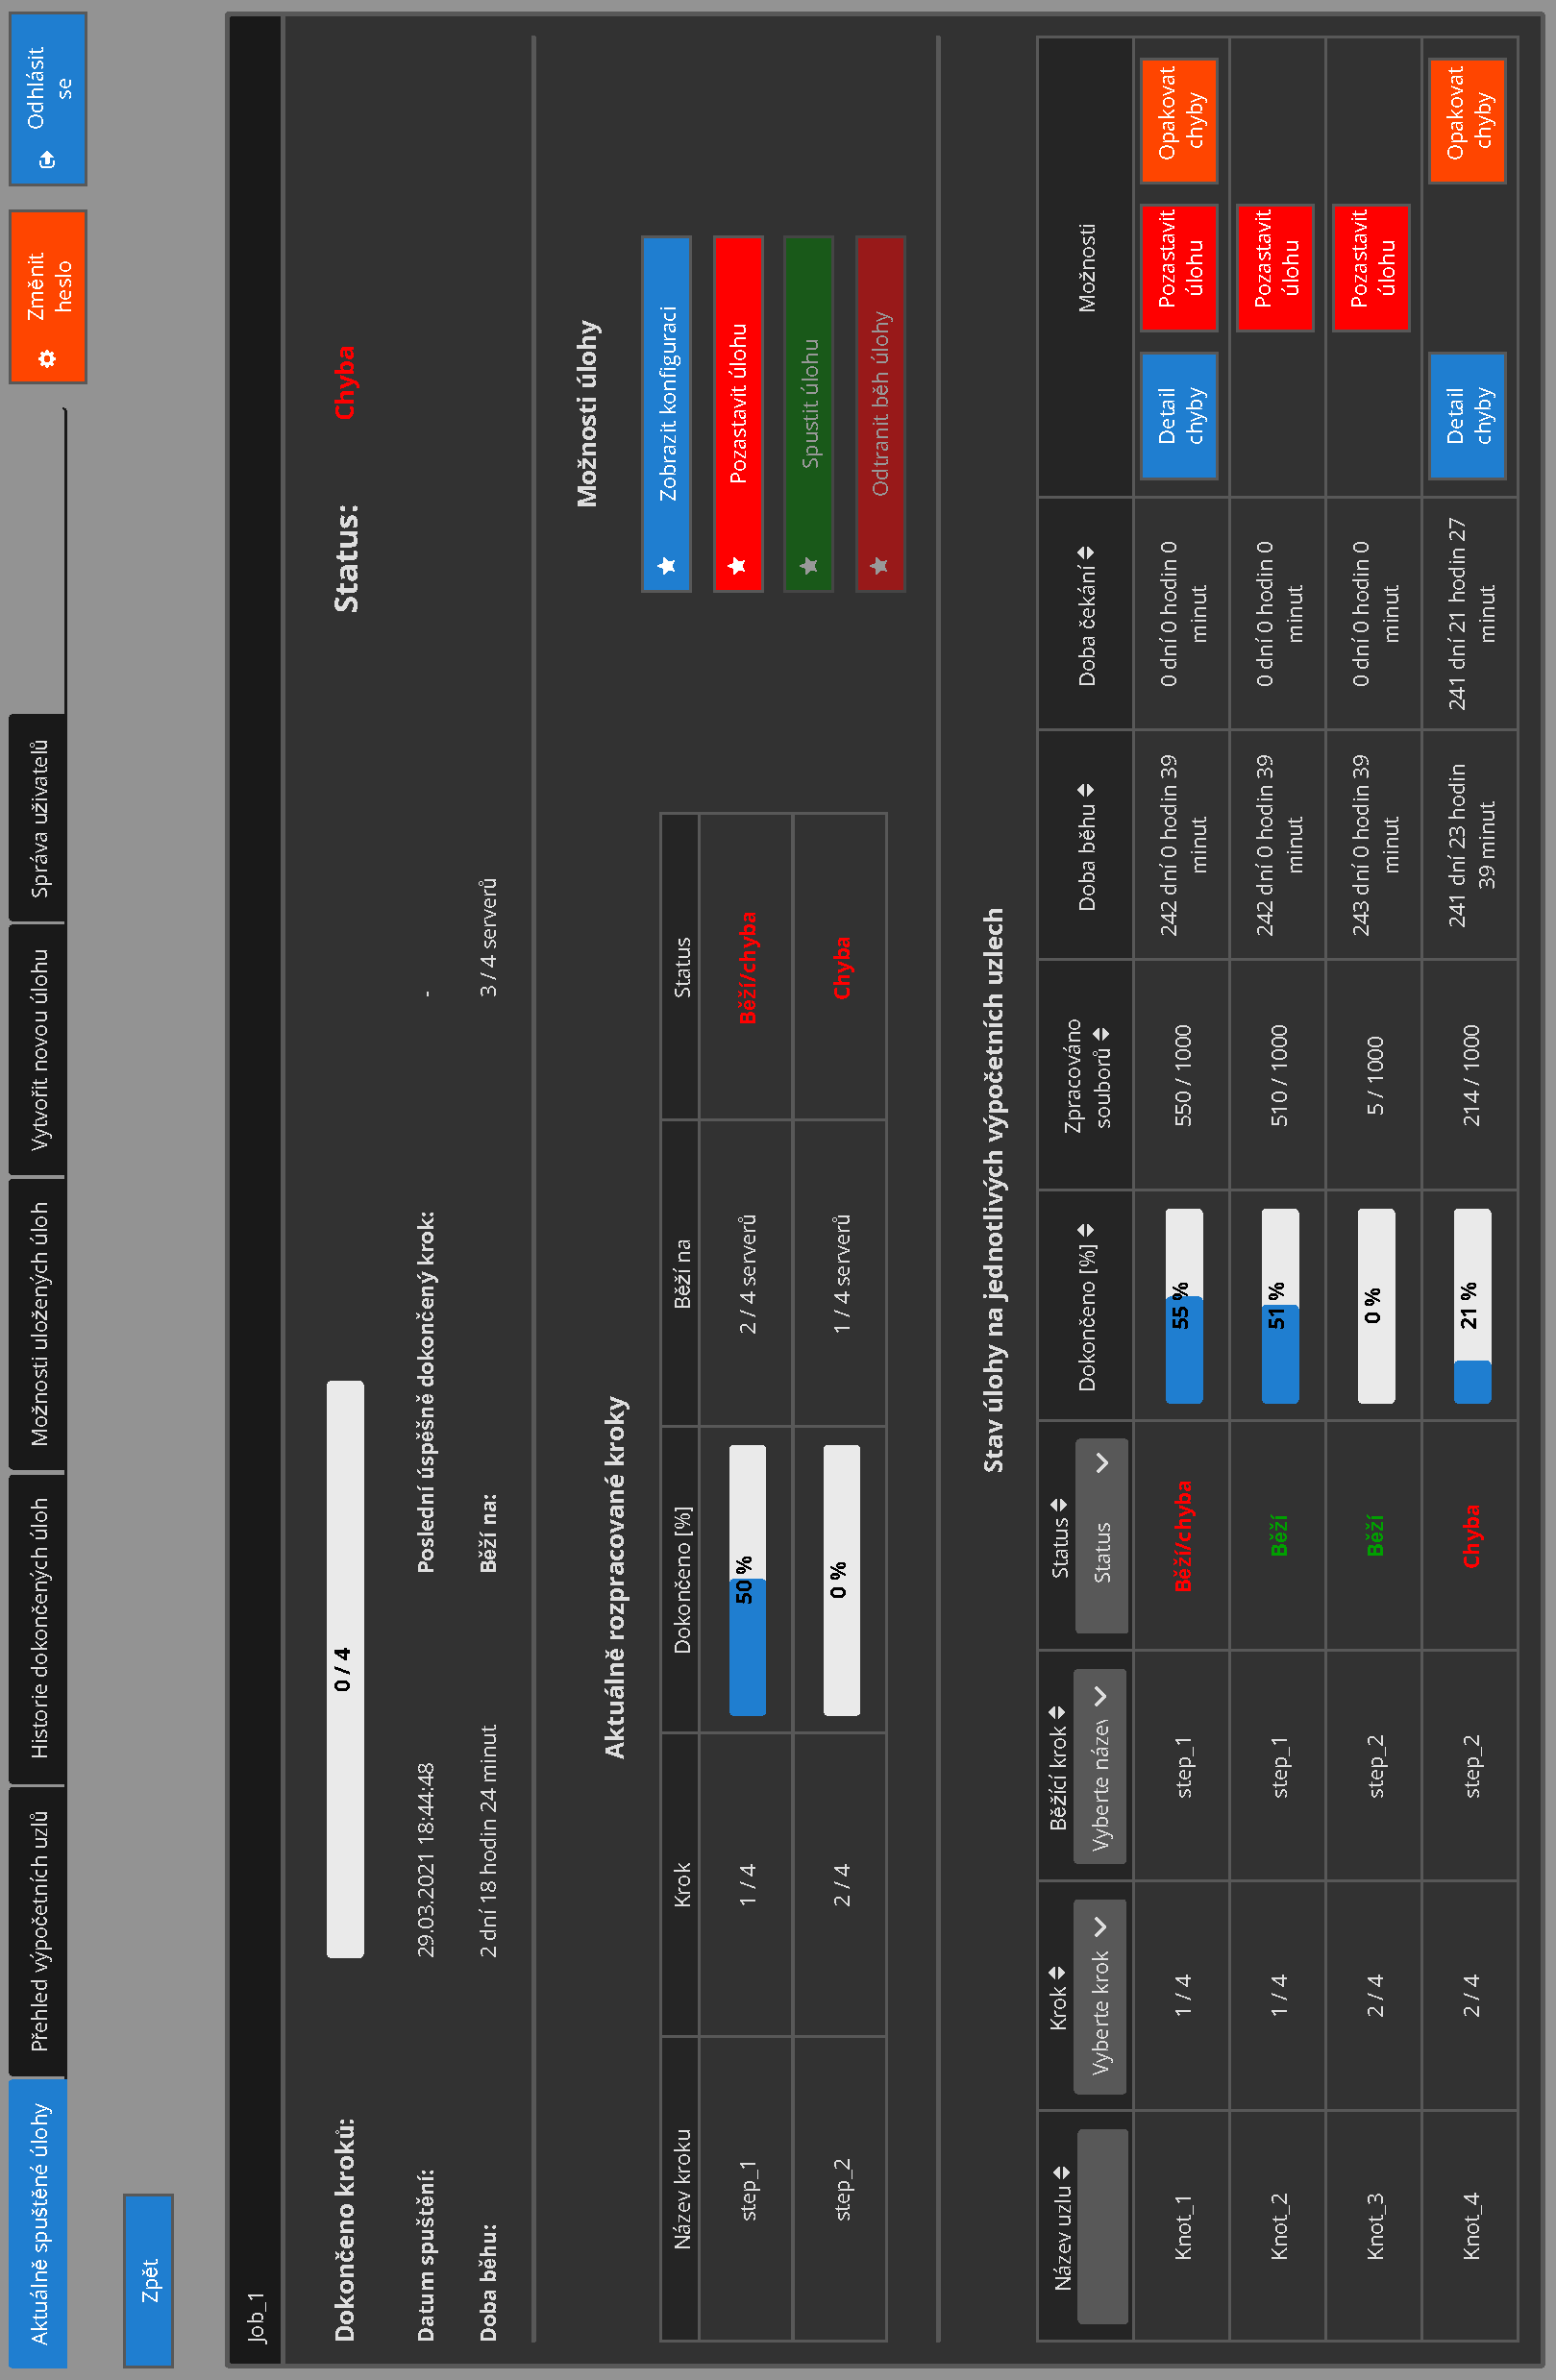
\includegraphics{images/RunTaskDetailAppDarkScreen.pdf}
        }
        \caption{\label{obr:runTaskDetailRealApp} {\it Snímek obrazovky detailu běžící úlohy reálné aplikace.}}
    \end{center}
\end{figure}

\section{Monitorování vytíženosti výpočetních uzlů}

Monitorování vytíženosti výpočetních uzlů je na centrálním uzlu implementováno pomocí Singleton EJB beanu, který periodicky každých 5~sekund u každého výpočetního uzlu ověřuje, zda je na něm nějaká výpočetní úloha spuštěna. Tyto hodnoty následně ukládá do databáze. Vytíženost výpočetního uzlu je ukládána v 5vteřinových, minutových, 30minutových, hodinových, 12hodinových a denních záznamech. Při každé periodické kontrole jsou 5vteřinové záznamy průměrovány po jednotlivých minutách. Do databáze je tak následně uložena jediná hodnota reprezentující průměrné vytížení výpočetního uzlu za danou minutu a 5vteřinové záznamy jsou odstraněny. Tyto minutové záznamy jsou dále průměrovány do delších časových úseků tak, aby bylo v grafech za jednotlivá období zobrazeno dostatečné množství dat a~zároveň nebyly kladeny příliš velké paměťové nároky pro ukládaná data. Pro jednotlivá časová období byla tedy stanovena tato rozlišení: 
\begin{itemize}
    \item Hodina -- graf obsahuje 60 hodnot vytíženosti výpočetního uzlu (rozlišení 1 minuta),
    \item Den -- Graf obsahuje 48 hodnot vytíženosti výpočetního uzlu (rozlišení 30~minut),
    \item Týden -- Graf obsahuje 168 hodnot vytíženosti výpočetního uzlu (rozlišení 1 hodina),
    \item Měsíc -- Graf obsahuje 60 hodnot vytíženosti výpočetního uzlu za posledních 30~dnů (rozlišení 12 h),
    \item 3 Měsíce -- Graf obsahuje 90~hodnot vytíženosti výpočetního uzlu za posledních 90~dnů (rozlišení 1~den),
    \item 6 Měsíců -- Graf obsahuje 180~hodnot vytíženosti výpočetního uzlu za posledních 180~dnů (rozlišení 1~den),
    \item Rok -- Graf obsahuje 365~hodnot vytíženosti výpočetního uzlu za posledních 365~dnů (rozlišení 1~den).
\end{itemize}

Denní záznamy, které jsou starší než 365~dnů, jsou z databáze automaticky odstraněny.

\section{Push notifikace}

Vzhledem k tomu, že uživatel komunikuje s centrálním uzlem pomocí bezstavového protokolu HTTP, bylo nezbytné při požadavku na zobrazení aktuálního stavu úlohy nebo výpočetních uzlů ručně obnovit stránku, aby mohla být načtena aktuální data. Pro vyřešení tohoto problému byly implementovány server push notifikace. Upozornění na nové události jsou zasílána uživatelům prostřednictvím 2~kanálů:
\begin{itemize}
    \item NODE\_EVENT\_CHANNEL -- kanál, na který je zaslána notifitikace v případě připojení/odpojení výpočetního uzlu nebo při vytvoření nových dat o obsazenosti některého výpočetního uzlu,
    \item RUN\_TASK\_EVENT\_CHANNEL -- kanál, na který je zaslána notifikace v případě jakékoliv změny v průběhu zpracování úlohy, tj. při chybě, spuštění, pozastavení nebo dokončení na některém výpočetním uzlu.
\end{itemize}

Při testování aplikace se ukázalo, že z důvodu chybné konfigurace úlohy při spuštění může dojít k tomu, že při zpracování každého vstupu úlohy na všech výpočetních uzlech nastane chyba, což způsobí vygenerování velkého množství notifikací. To bylo nevýhodné zejména z důvodu velkého zatěžování sítě. Data byla navíc obnovena do aktuálního stavu již při první nebo druhé notifikaci. Všechny ostatní tak byly zcela zbytečné. Aby se zamezilo tomuto problému, bylo pro jejich odesílání vytvořeno samostatné vlákno, které je spouštěné pravidelně každou vteřinu. Požadavek na notifikaci uživatele je realizován formou nastavení příznaku. Pokud je tedy během jedné vteřiny vytvořeno více notifikací, je ve skutečnosti uživateli zaslána pouze jediná notifikace na odpovídající kanál.

\section{Nasazení aplikace}

V této kapitole je popsán postup nasazení aplikace pro centrální uzel na aplikační server Glassfish včetně všech parametrů, které je nezbytné před nasazením nastavit. Dále je zde uveden postup spuštění aplikace pro výpočetní uzel včetně formátu konfiguračního souboru a argumentů, se kterými se program spouští.

\subsection*{Nasazení aplikace pro centrální uzel}

Po stažení repozitáře je před sestavením aplikace pro centrální uzel nutné v souboru \textit{web.xml} nastavit hodnoty těchto parametrů:
\begin{itemize}
    \item \textit{PATH\_TO\_ERR\_LOG} -- absolutní cesta pro uložení logovacího souboru aplikace pro centrální uzel,
    \item \textit{SOCKET\_LISTENING\_PORT} -- číslo portu, na kterém budou přijímána spojení s~výpočetními uzly,
    \item \textit{IS\_ALIVE\_SENDING\_PERIOD} -- časová perioda v~sekundách, v~jaké budou pravidelně odesílány zprávy typu \textit{IsAliveMsg} na výpočetní uzel,
    \item \textit{RECORD\_TIME\_ZONE} -- časové pásmo, ve kterém mají být ukládány a~zobrazovány záznamy o~využití výpočetních uzlů.
\end{itemize}

Dále je nutné v souboru \textit{hibernate.cfg.xml} nastavit údaje pro připojení k databázi MySQL, tj. URL, uživatelské jméno a heslo. Po nastavení těchto parametrů je možné celou aplikaci sestavit a výsledný soubor \texttt{war} nasadit na aplikační server.

\subsection*{Nasazení aplikace pro výpočetní uzel}

Aplikaci pro výpočetní uzel stačí po stažení repozitáře jednoduše sestavit. Program se spouští se 4~povinnými argumenty:
\begin{itemize}
    \item \textit{-config, -{}-pathToConfig <arg>} -- absolutní cesta ke konfiguračnímu souboru,
    \item \textit{-ip, -{}-primaryIP <arg>} -- IP adresa, na které přijímá centrální uzel spojení s výpočetními uzly,
    \item \textit{-port, -{}-primaryPort <arg>} -- číslo portu, na kterém přijímá centrální uzel spojení s~výpočetními uzly,
    \item \textit{-name, -{}-secNodeName <arg>} --  název výpočetního uzlu.
\end{itemize}

Konfigurační soubor musí být ve formátu JSON a~má následující formát:
\vspace{0.6cm} \newline
\hspace*{1.5cm}\{  \newline
    \hspace*{2cm} "pathToLogFolder" : "\textit{<value>}", \newline
    \hspace*{2cm} "isAliveSendingPeriod" : \textit{<value>} \newline
    \hspace*{2cm} "pathToBashConfigFolder" : "\textit{<value>}"  \newline
\hspace*{1.5cm}\}
\vspace{0.6cm}

První položka, \textit{pathToLogFolder}, specifikuje absolutní cestu ke složce, kde bude uložen logovací soubor, přičemž název souboru bude odvozen od názvu výpočetního uzlu. Druhý parametr, \textit{isAliveSendingPeriod}, pak určuje časovou periodu v~sekundách, v~jaké budou pravidelně odesílány zprávy typu \textit{IsAliveMsg} na centrální uzel. Poslední parametr, \textit{pathToBashConfigFolder}, představuje cestu ke složce, ve které je umístěn konfigurační soubor s~názvem \textit{.toprc} určující formát výstupu pro program \textit{Top}.

Vzhledem k tomu, že je komunikace mezi centrálním a~výpočetním uzlem šifrovaná, je při spuštění navíc nutné zadat cestu k souboru s~certifikátem centrálního uzlu, resp. aplikačního serveru, na kterém aplikace běží, a~to nastavením systémové proměnné \textit{javax.net.ssl.trustStore}. Dále je nutné specifikovat heslo pro přístup k~tomuto souboru, a~to~nastavením systémové proměnné \textit{javax.net.ssl.trustStorePassword}. Aplikace pro výpočetní uzel se tedy spustí pomocí následujícího příkazu:

\texttt{java --Djavax.net.ssl.trustStore=}\textit{<path\_to\_truststore>} \newline 
\hspace*{1.5cm} \texttt{--Djavax.net.ssl.trustStorePassword=}\textit{<trustore\_password>} \newline
\hspace*{1.5cm} \texttt{--jar} \hspace*{0.45cm} \textit{<path\_to\_jar\_file>} \newline
\hspace*{1.5cm} \texttt{--ip} \hspace*{0.65cm} \textit{<primary\_node\_ip\_address>} \newline
\hspace*{1.5cm} \texttt{--port} \hspace*{0.25cm} \textit{<primary\_node\_port\_number>} \newline
\hspace*{1.5cm} \texttt{--name} \hspace*{0.25cm} \textit{<node\_name>} \newline
\hspace*{1.5cm} \texttt{--config} \textit{<path\_to\_config\_file}

%%%%%%%%%%%%%%%%%%%%%%%%%%%%%%%%%%%%%%%%%%%%%%%%%%%%%%%%%%%%%%%%%%%%%%%%%%%%%%%%%%%%%%%%%%%%%%%%%%%%%%%%%%%%%%%%%%

\chapter{Testování}
\label{chapter:testing}
V této kapitole je popsán způsob automatizovaného testování aplikace pro výpočetní uzel pomocí jednotkových testů. Následně je uveden postup testování celého systému.

\section{Testování aplikace pro výpočetní uzel}
\label{section:testingSecondaryNode}

Pro aplikaci určenou k nasazení na výpočetní uzly byly vytvořeny jednotkové testy s využitím frameworku JUnit, který je popsán v kapitole \ref{chapter:used_technologies}. Tyto jednotkové testy jsou zaměřeny na testování všech vstupně/výstupních operací a validací prováděných po dokončení zpracování každého vstupu zpracovávaného kroku úlohy. 

Za účelem otestování celé aplikace pro výpočetní uzel byly vytvořeny skripty v jazyce Python simulující úlohu, u které se očekává:
\begin{itemize}
    \item úspěšné zpracování,
    \item překročení maximální doby zpracování jednoho vstupu,
    \item chyba neočekávaného vstupu,
    \item chyba výstupní validace,
    \item úspěšné pozastavení a následné opětovné spuštění úlohy,
    \item úspěšné pozastavení a následné úspěšné spuštění opětovného zpracování chybných vstupů,
    \item úspěšné spuštění opětovného zpracování chybných vstupů u běžící úlohy.
\end{itemize}

Aby bylo možné tyto testovací úlohy automatizovaně spouštět, bylo v rámci těchto testů nezbytné vytvořit testovací server simulující reálný centrální uzel, který slouží pro zaslání požadavku na zpracování dané testovací úlohy a přijímání zpráv z testované aplikace pro výpočetní uzel.

\section{Testování systému}

Testování celého systému bylo rozděleno do několika částí. V první části byla úloha testována lokálně s jedním výpočetním uzlem -- na daném stroji byl tedy spuštěn jak aplikační server centrálního uzlu, tak aplikace pro výpočetní uzel. V této konfiguraci byly spuštěny stejné úlohy, jako v případě použití testovacího serveru, které jsou popsané v kapitole \ref{section:testingSecondaryNode}, nyní však s reálným aplikačním serverem. 

Následně byla celá aplikace nasazena na aplikační server Výzkumné skupiny znalostních technologií. Po zprovoznění aplikace byly nejprve prováděny testy, které při lokálním spuštění nebylo možné provést. Jednalo se o testování korektního přijetí a odmítnutí spojení s výpočetním uzlem při výpadku a opětovném připojení výpočetního uzlu. Rovněž bylo ověřeno korektní odmítnutí spojení při připojení uzlu z jiné IP adresy nebo s názvem uzlu, se kterým je již připojen jiný výpočetní uzel. Následně byly spuštěny úlohy uvedené v kapitole \ref{section:testingSecondaryNode}, ke kterým však byly přidány kroky obsahující synchronizaci, a testovalo se tak, zda dojde při zpracování synchronizačního kroku k čekání na zpracování úlohy na všech výpočetních uzlech a následně k automatickému pokračování ve zpracování. Dále bylo testováno spuštění několika úloh zároveň na stejných výpočetních uzlech. Tímto způsobem se ověřovalo, zda při přerušení zpracování jedné úlohy z důvodu dokončení, chyby nebo z~důvodu čekání na synchronizačním kroku dojde k automatickému spuštění v pořadí další nezpracované úlohy a následně, tj. po odstranění chyby nebo splnění podmínky synchronizace, dojde po dokončení rozpracovaného vstupu opět k pokračování předchozí úlohy. Při tomto testování se ukázalo jako nedostatečné využívat pro správu připojení k databázi výchozí connection pool ve frameworku Hibernate. Pokud nastala chyba na více výpočetních uzlech současně, chtěla všechna vlákna udržující spojení s těmito výpočetními uzly ukládat data o chybě do databáze. Tím došlo k vyčerpání maximálního počtu spojení s databází, jelikož nebyl výchozí connection pool při takovém vytížení schopen jednotlivá spojení mezi tato vlákna efektivně rozdělovat. Tento problém byl vyřešen využitím knihovny C3P0 pro správu spojení s databází, která je popsána v kapitole \ref{subsection:technology_C3P0}.

Jakmile byly všechny předchozí testy úspěšně provedeny, bylo spuštěno zpracování úlohy definované Výzkumnou skupinou znalostních technologií nad daty z projektu Common Crawl na všech 59~výpočetních uzlech. Tato úloha sestávala ze 3 kroků -- vertikalizace, deduplikace a syntaktická analýza. Při spuštění úlohy se zjistilo, že zpracování některých vstupů skončilo s chybou, přičemž jejich zpracování nebylo možné dokončit ani po opětovném spuštění, jelikož byl vstupní archiv chybně zkomprimován. Řízení zpracování úlohy bylo na základě tohoto zjištění doplněno o~možnost přeskočit zpracování těchto chybných vstupů. 

V grafu \ref{obr:executedTimeGraphs}a je možné vidět dobu zpracování každého kroku úlohy na jednotlivých výpočetních uzlech. Na všech výpočetních uzlech bylo zpracováváno 228 vstupních souborů s~výjimkou serveru \textit{athena1}, kde bylo k dispozici pouze 66 souborů. Z diagramů je zřejmé, že první krok, vertikalizace, byl nejdéle zpracováván na uzlu \textit{minerva2}, kde úloha běžela 124 hodin. Druhý krok, deduplikace, běžel nejdéle na uzlu \textit{athena12}, kde zpracování trvalo 12~hodin. Poslední krok, syntaktická analýza, běžela nejdéle na uzlu \textit{knot09}. Zpracování všech vstupních souborů na tomto uzlu trvalo 14 hodin. Při původním způsobu spuštění úlohy by byl následující krok úlohy spuštěn vždy až po dokončení předchozího kroku na všech výpočetních uzlech, jak je popsáno v kapitole \ref{section:act_way_of_running_tasks}. Celková doba trvání úlohy by se tak rovnala součtu maximálních dob zpracování každého kroku úlohy. V případě této úlohy by tedy zpracování trvalo celkově 160 hodin.

\begin{figure}[H]
    \begin{center}
        \scalebox{0.8}
        {
            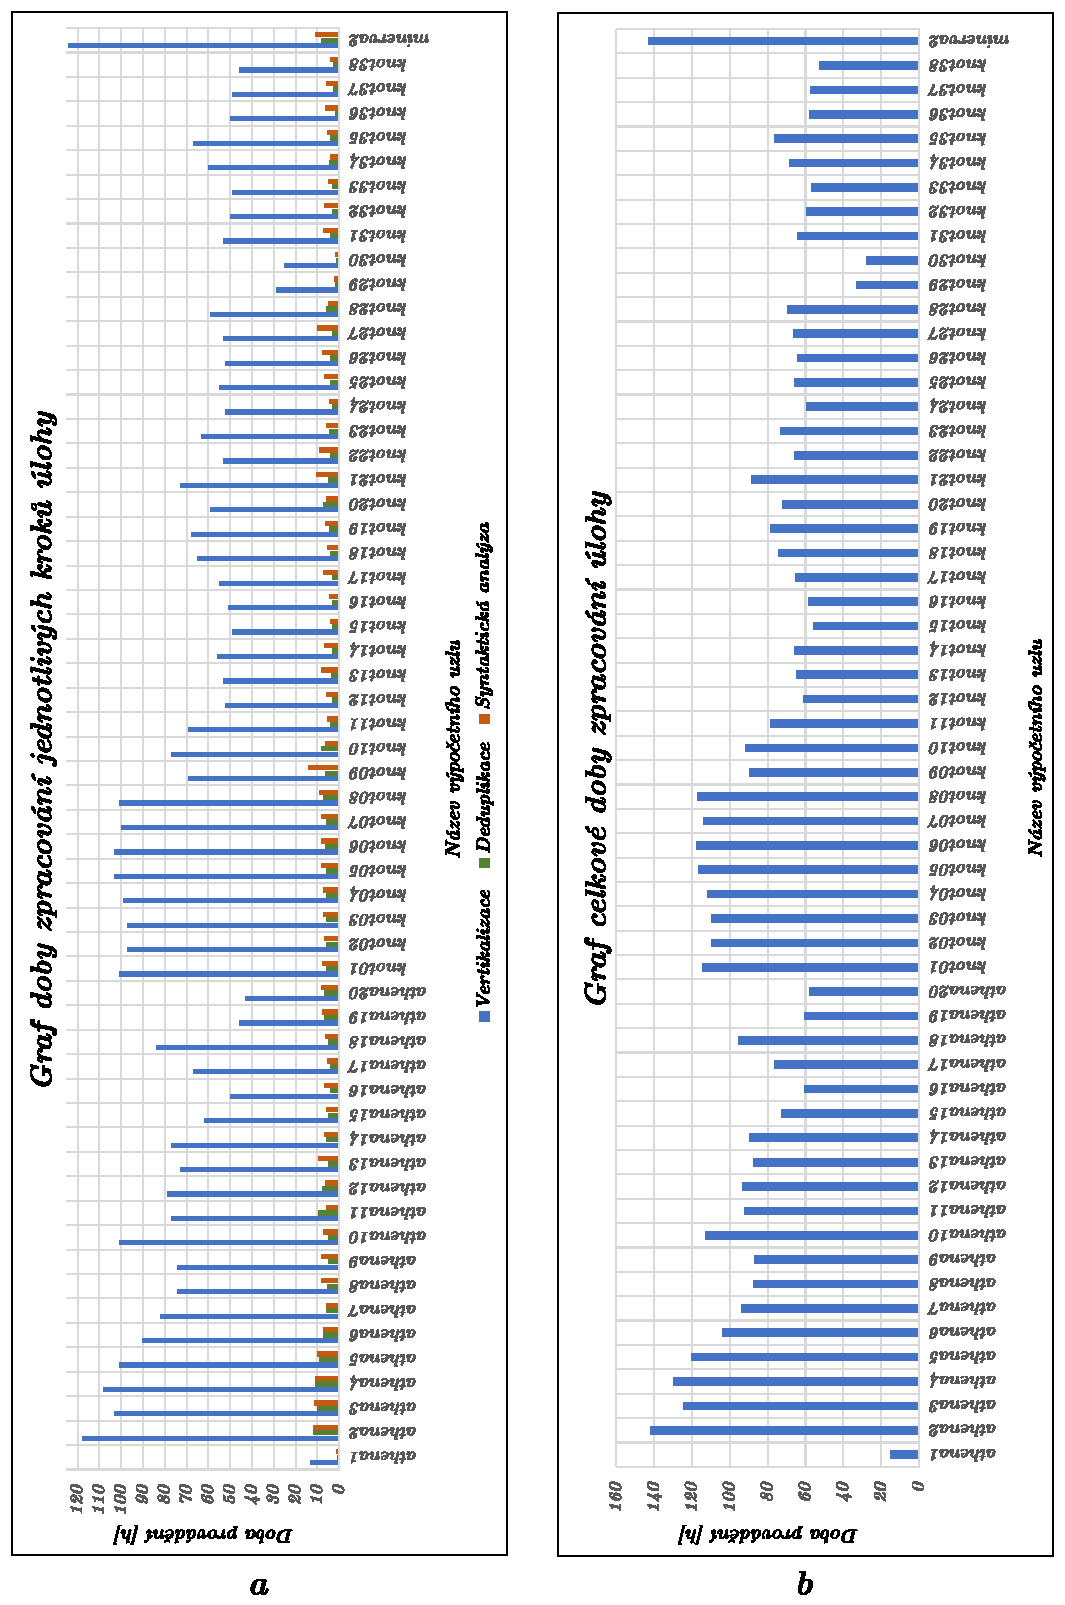
\includegraphics{images/ExecutedTimeGraphs.pdf}
        }
        \caption{\label{obr:executedTimeGraphs} {\it Graf znázorňující dobu zpracování úlohy nad daty z projektu Common Crawl na jednotlivých výpočetních uzlech.}}
    \end{center}
\end{figure}
Celkovou dobu trvání úlohy na jednotlivých výpočetních uzlech je možné vidět v grafu \ref{obr:executedTimeGraphs}b. Je zřejmé, že zpracování nejdéle trvalo na výpočetním uzlu \textit{minerva2}, kde byla celková doba běhu úlohy 143~hodin. Celková doba provádění úlohy tak byla v porovnání s dřívějším způsobem spouštění~o~17 hodin kratší. Tohoto zrychlení však bylo dosaženo také díky tomu, že každý krok úlohy byl nejdéle zpracováván na jiném uzlu. Pokud by všechny 3~kroky úlohy byly nejdéle zpracovávány na stejném výpočetním uzlu, trvalo by zpracování stejně dlouho, avšak výpočetní výkon uzlů, které by čekaly na pomalejší výpočetní uzly, by mohl být použit pro zpracování jiné úlohy. Z grafu dále vyplývá, že doba zpracování je na výpočetních uzlech velmi různorodá. Pokud zanedbáme uzel \textit{athena1}, který zpracovával menší množství souborů, je rozdíl mezi nejdelší a nejkratší dobou zpracování úlohy 115 hodin. Tím se tedy potvrdily předpoklady ze zkušeností Výzkumné skupiny znalostních technologií, kdy při dosavadním způsobu zpracování docházelo k velkému plýtvání výpočetním výkonem, jelikož uzel \textit{athena1} musel dříve 115 hodin čekat na dokončení zpracování úlohy na uzlu \textit{minerva2}.

%%%%%%%%%%%%%%%%%%%%%%%%%%%%%%%%%%%%%%%%%%%%%%%%%%%%%%%%%%%%%%%%%%%%%%%%%%%%%%%%%%%%%%%%%%%%%%%%%%%%%%%%%%%%%%%%%%

\chapter{Závěr}
\label{chapter:conclusion}

V rámci této diplomové práce byl nastudován současný způsob zpracování paralelních úloh ve Výzkumné skupině znalostních technologií. Analýza odhalila nedostatky a problémy tohoto řešení, na základě nichž byly stanoveny požadavky na novou aplikaci. Poté byly nastudovány existující nástroje umožňující řízení a monitorování paralelního zpracování dat. Hlavní pozornost byla věnována nástrojům, které již byly ve Výzkumné skupině znalostních technologií testovány, a nevýhodám, které jejich nasazení odhalilo. Následně byl na základě požadavků proveden návrh celého systému skládajícího se ze dvou částí~--~aplikace pro výpočetní uzel a aplikace pro centrální uzel. Nejprve bylo navrženo grafické uživatelské rozhraní webové aplikace pro centrální uzel, což vedlo k získání upřesňujících požadavků. Poté byl proveden návrh uložení dat v databázi a struktury obou aplikací. Nakonec byl navržen způsob komunikace centrálního a~výpočetního uzlu. Následně byly obě aplikace implementovány dle návrhu. Nakonec byl celý systém nasazen a otestován na serverech Výzkumné skupiny znalostních technologií. 

Při zpracování úlohy nad daty z projektu Common Crawl se zjistilo, že by úloha předchozím způsobem spouštění běžela 160 hodin. S využitím nově vytvořeného systému byla celková doba zpracování o 17 hodin kratší. Výsledná úspora času je však závislá na tom, na jakém uzlu bylo zpracování každého kroku nejpomalejší. Během testování se také potvrdily předpoklady velmi rozdílné doby zpracování kroků úlohy na jednotlivých výpočetních uzlech. Předchozím způsobem spouštění tak docházelo k velkému plýtvání výpočetním výkonem, jelikož zpracování každého kroku úlohy mohlo být spouštěno až po dokončení předchozího kroku na všech uzlech. Vytvořený systém umožňuje definovat více úloh současně. Při čekání na pomalejší uzel tak může být zpracovávána jiná úloha, čímž dochází k~mnohem lepšímu využití výpočetního výkonu. Aplikace poskytuje uživateli přehled o všech běžících úlohách a~o~stavu všech připojených výpočetních uzlů s využitím minimální režie, což patří mezi hlavní přínosy oproti předchozímu řešení, jelikož režie byla hlavním problémem u~dříve testovaných nástrojů pro distribuované zpracování dat.
\enlargethispage{2\baselineskip}

V budoucnu bych chtěl zobrazení chyb, které nastaly při zpracování úlohy, rozšířit o~možnost exportovat si tyto chyby do souboru, jelikož se při testování zjistilo, že zpracování některých vstupů skončí s neopravitelnou chybou. Při zpracování jiné úlohy by se tak na základě exportovaných dat o chybách mohly tyto vstupy vynechat, čímž by došlo k další úspoře výpočetního výkonu. Dále bych chtěl vytváření úlohy rozšířit o~možnost definovat počet procesů, ve kterých má být úloha spuštěna, pro každý výpočetní uzel zvlášť, jelikož mají výpočetní uzly rozdílné počty procesorů. U definice úlohy bych chtěl také přidat možnost záměny pořadí jednotlivých částí sestavovaného příkazu. V tuto chvíli je totiž pevně dáno pořadí argumentů vstupu a výstupu, což by mohlo znemožnit spuštění programů využívajících poziční argumenty.
\enlargethispage{\baselineskip}